\documentclass[a4paper,12pt]{report}
\usepackage{graphicx}
\usepackage{cancel}	%para cancelar expresiones en fórmulas
\usepackage{multicol}
\usepackage{multirow}
\usepackage{amsmath}
\usepackage{float}
\usepackage{url}
\usepackage{color}
\usepackage{tablefootnote}
\usepackage[12pt]{moresize}	%más tamaños de letra
\usepackage{bm}	%bold para math

\usepackage{titlesec}
\titleformat{\chapter}[display]
{\normalfont\bfseries}{}{0pt}{\Huge}	%quitar header de chapter

\usepackage{siunitx}	%support for units, numbers
\sisetup{output-decimal-marker={.}, separate-uncertainty}

\usepackage{hyperref}
\hypersetup{
	colorlinks=true,
	linkcolor=blue,
	citecolor=red,
	bookmarksopen=true,
	bookmarksopenlevel=1,
	urlcolor=blue
}

\usepackage{tikz}	%%TIKZ for drawings, shapes
\usetikzlibrary{positioning}
\tikzset{
	nodo/.style={
		rectangle,
		draw,
		black,
		thick,
		rounded corners,
		node distance=1.5cm,
		inner sep=0.3cm,
		font=\large
	}
}

%%% NOMBRES DE COSAS
\renewcommand{\abstractname}{Abstract}
\renewcommand{\figurename}{Figure}
\renewcommand{\tablename}{Table}
\renewcommand{\contentsname}{Table of Contents}
\renewcommand{\appendixname}{Appendix}
\renewcommand{\bibname}{References}
\renewcommand{\chaptername}{Part}

%%% COMANDOS COMUNES
\newcommand{\dif}{\text{d}}
\newcommand{\ddt}[1]{\frac{\dif #1}{\dif t}}
\newcommand{\der}[2]{\frac{\dif #1}{\dif #2}}
\newcommand{\mder}[3]{\frac{\dif^{#3}#1}{\dif #2^{#3}}}		%derivada múltiple
\newcommand{\norm}[1]{\left\| #1 \right\|}
\newcommand{\an}{($\alpha$,n) }
\newcommand{\Aliso}{\textsuperscript{27}Al }
\newcommand{\Piso}{\textsuperscript{30}P }
\newcommand{\Na}{\textsuperscript{22}Na }

%%%%%%%%%%%%%%%%%%%%%%%%%%%%%%%%%%%%%%%%%%%%%%%%%%%%%%%%%
\usepackage[a4paper]{geometry}
\geometry{top=2cm,bottom=2cm,left=1.8cm,right=1.8cm}
\usepackage{setspace}	%interlineado
\onehalfspace	%interlineado 1.5

\makeindex
%%%%%%%%%%%%%%%%%%%%%%%%%%%%%%%%%%%%%%%%%%%%%%%%%%%%%%%%%
\begin{document}
\begin{titlepage}
	\centering
	\Huge Inter-University Master's degree in Nuclear Physics\par
	\vspace*{3cm}
	\HUGE \textbf{Measurements of ($\bm{\alpha}$,n) reactions in CNA/HISPANOS}\par	%TBD? más largo?
	\vspace{1cm}
	
\includegraphics[width=0.35\textwidth]{us.png}\\
	\vspace{1cm}
	\Large \textsc{Erik Cárdenas Mayoral}\par
	\vspace{2cm}
	Supervisors:\\
	Carlos Guerrero Sánchez\\
	María Begoña Fernández Martínez\par
	\vfill
	26/06/2023
\end{titlepage}

\begin{abstract}
English abstract.
\\
Abstract español.
\end{abstract}

\tableofcontents

\chapter{Introduction and motivation}
·Explain what \an reactions are.\\

·Relevance of \an reactions for: dark matter search, astrophysics.\\

·Actual state and types of \an measurements.\\

·The objective of the measurements at CNA are to check the viability for carrying out more \an measurements.\\


\chapter{Experimental setup and procedure}
\section{Setup}
The source of alphas for the experiment is the \qty{3}{\mega\volt} tandem accelerator at CNA, which fires alphas at a \Aliso target.
Detectors used are both organic and inorganic scintillators.

\begin{figure}[H]
	\centering
	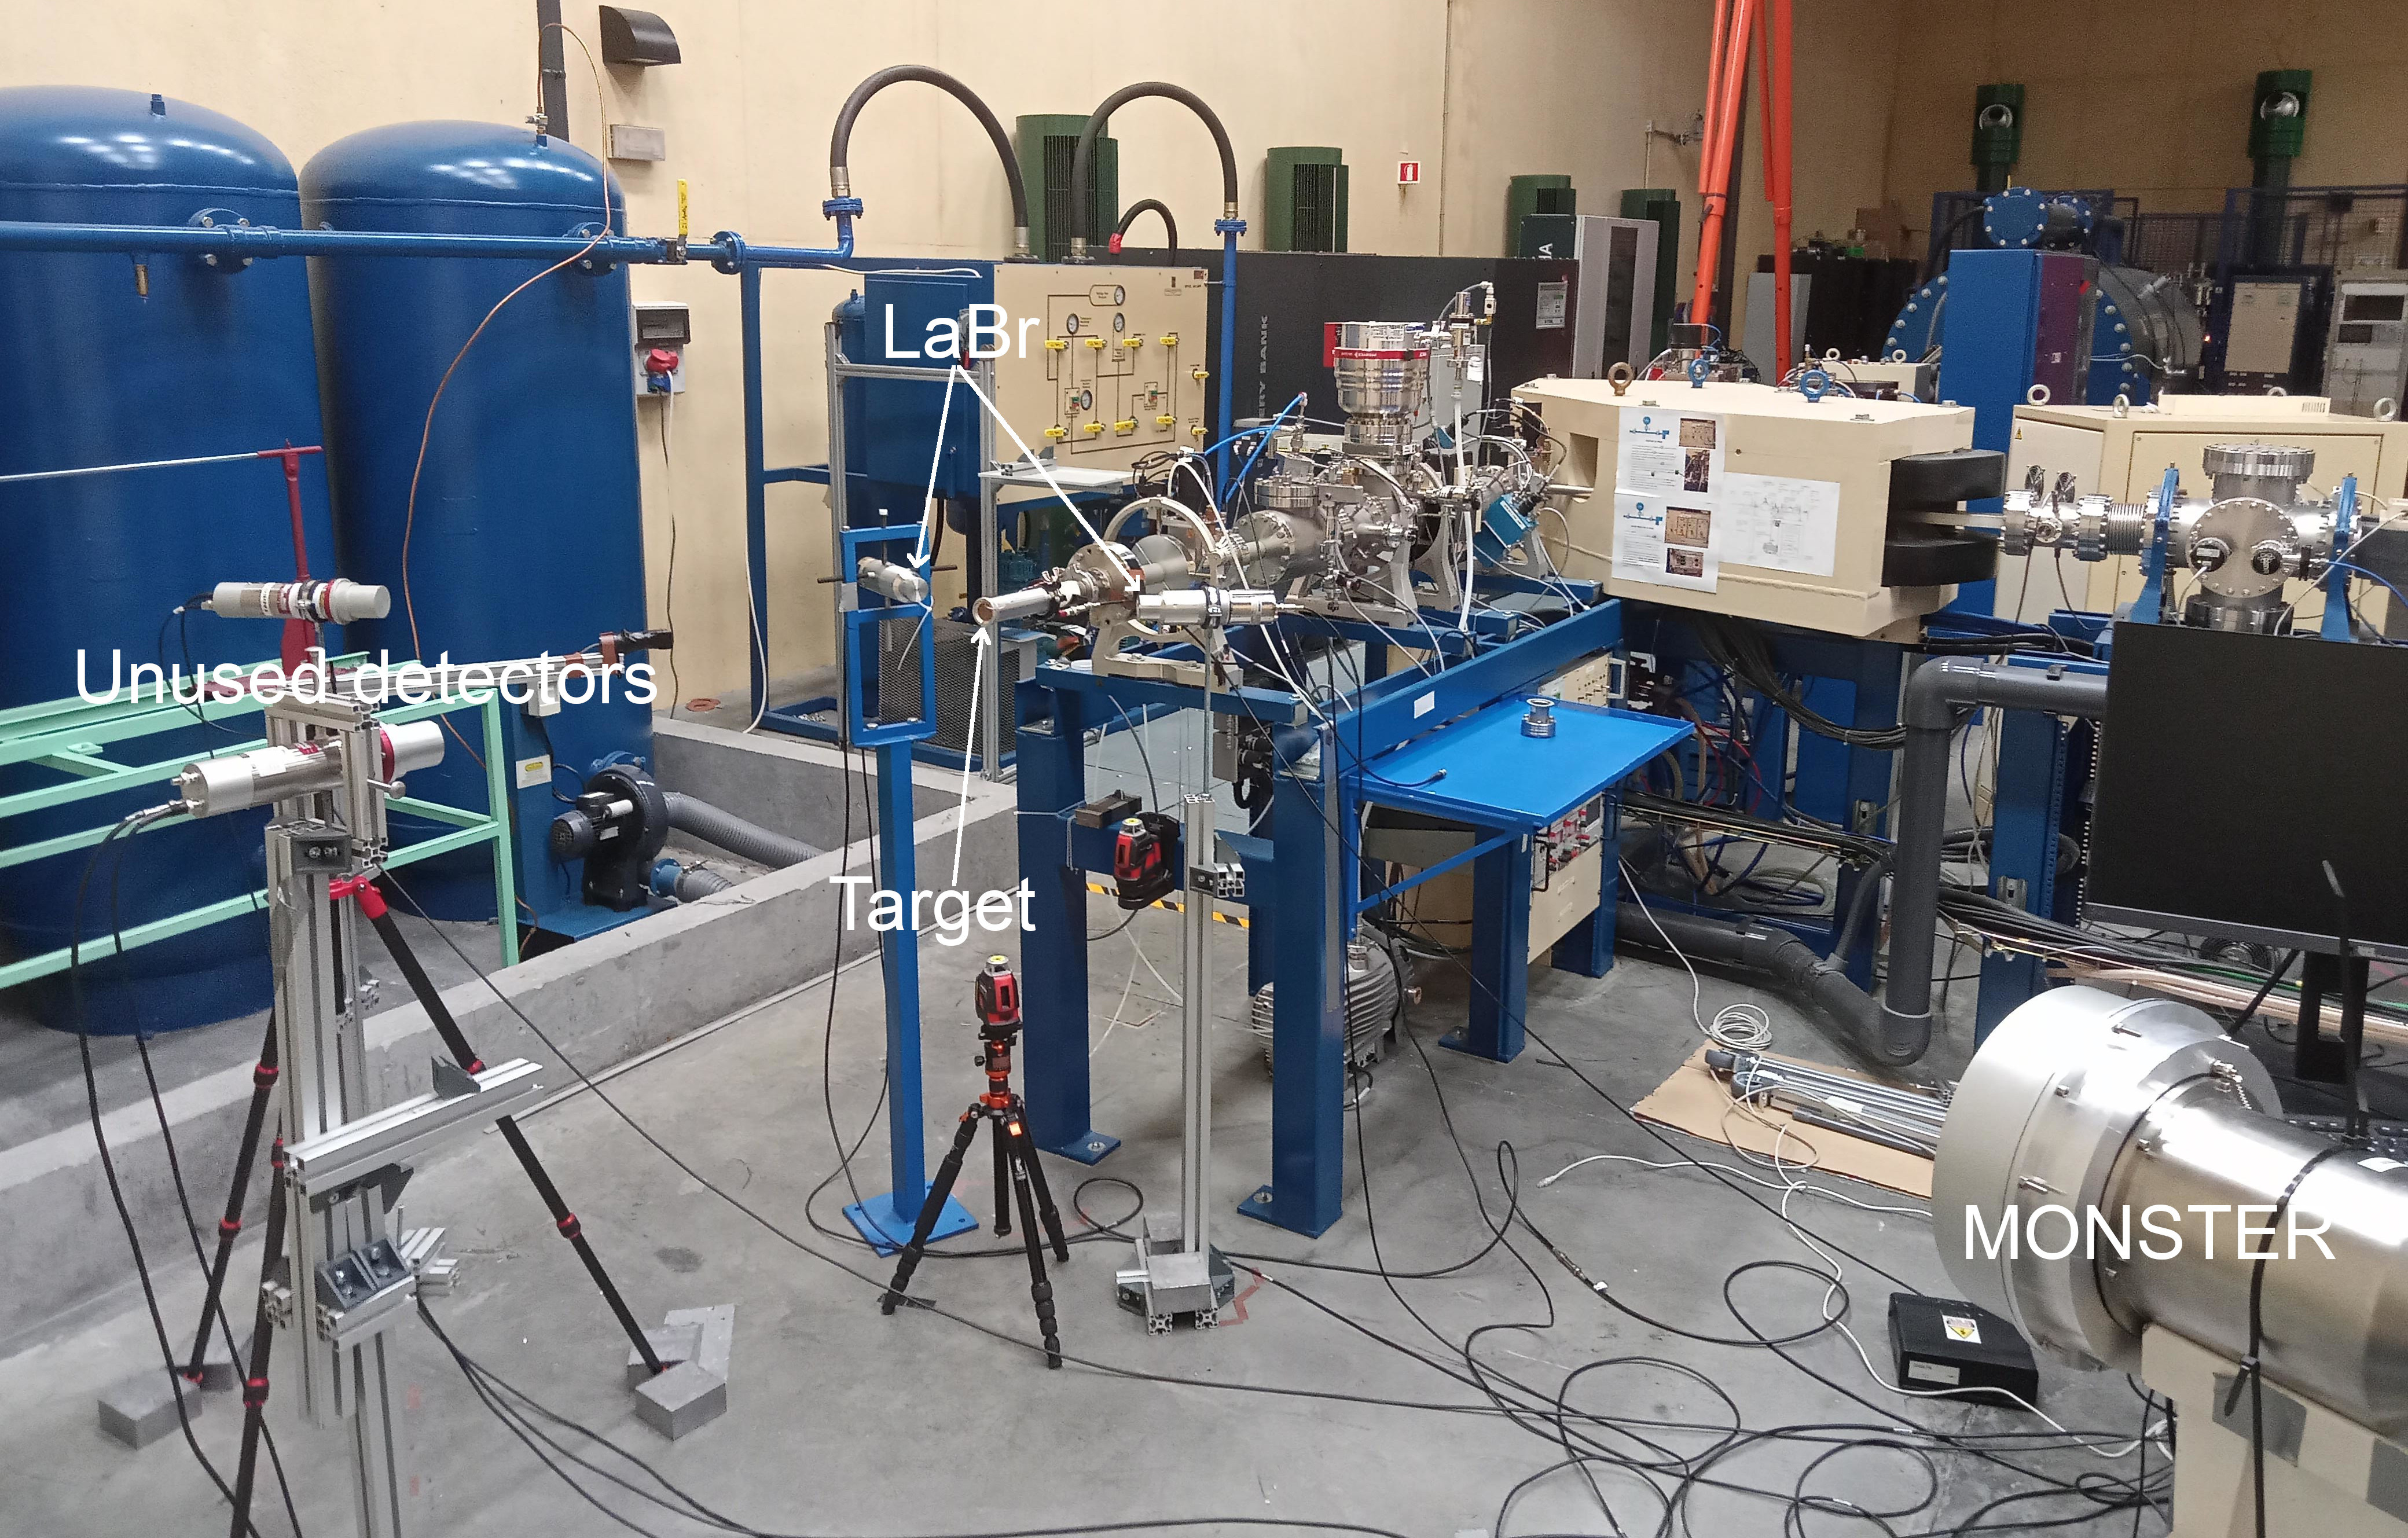
\includegraphics[width=\textwidth]{overview_photo.jpg}
	\caption{Overview picture of the experimental setup.
	Detectors and the target are labeled.}
	\label{overview_photo}
\end{figure}

\subsection{Tandem 3MV accelerator}
A tandem is a type of linear particle accelerator whose main characteristic is that particles are accelerated twice by the same terminal voltage.
Particles are injected with negative charge from a source situated outside the tank, and accelerated toward the terminal.

Once the negatively charged particles arrive a the terminal, their electrons are removed by a gas, called the \textit{stripper}.
Now with a positive charge, they are accelerated the rest of the way by the same voltage.
\\

In the case of alpha particles, they are injected with charge -1, and then stripped of all electrons, to charge +2.
Given that the maximum voltage of the CNA tandem accelerator is \qty{3}{\mega\volt}, alphas can be accelerated to a maximum of $3\cdot\left(1+2\right) = \qty{9}{\mega\eV}$.	%TBD:añadir injection energy
\\

·Explain pulsed mode: chopper, buncher.\\
·Explain the different parts of the neutron line. Photos.\\
·Difficulty of using alphas with the accelerator, with it being designed for deuterons. Graph of gamma flash highlighting assymetry and tail.\\

\subsection{Target}
The target is a sheet of \qty{95}{\percent} purity \Aliso.	%TBD:confirmar porcentaje
This metal was chosen because it is relatively well known compared to others, with the best available measurements of \an reactions to compare to.
\\

Because the target is thick (more than a few micrometers), all of the alphas will be completely stopped by it.
This means that, for some of the \an reactions, the alpha particles will have lost part of their energy in the material.

Any measurements taken with a thick target are thus integrated measurements, for energies up to the one the alphas were accelerated to.
If we wanted to measure only \an reactions at a specific energy, we would have to use a very thin sheet of aluminium, so as to stop the alphas from being slowed down.
\\

It is important, in order to obtain quantitative results, to know how many alphas hit the target.
Because they are stripped of all their electrons, they have charge +2 when they arrive at the target.\footnote{Because the neutron line is aligned with the accelerator, using the \qty{90}{\degree} electromagnet to eliminate other charge states is not possible. Nontheless, the number of alpha particles with charge +1 is considered small enough as to be ignored.}
The target is not grounded, and so it charges up positively as alphas impact it.
By measuring the charge on the target, we can know how many alphas have hit it.

To do so, we connect the target via a copper wire to a \emph{charge integrator}, a device that emits a pulse and discharges the target each time it reaches \qty{0.1}{\nano\coulomb}, or approximately \num{3E8} alphas.
It is important that the target does not accumulate too much positive charge, as that could slow down or deflect incoming particles.

\begin{figure}[H]
	\centering
	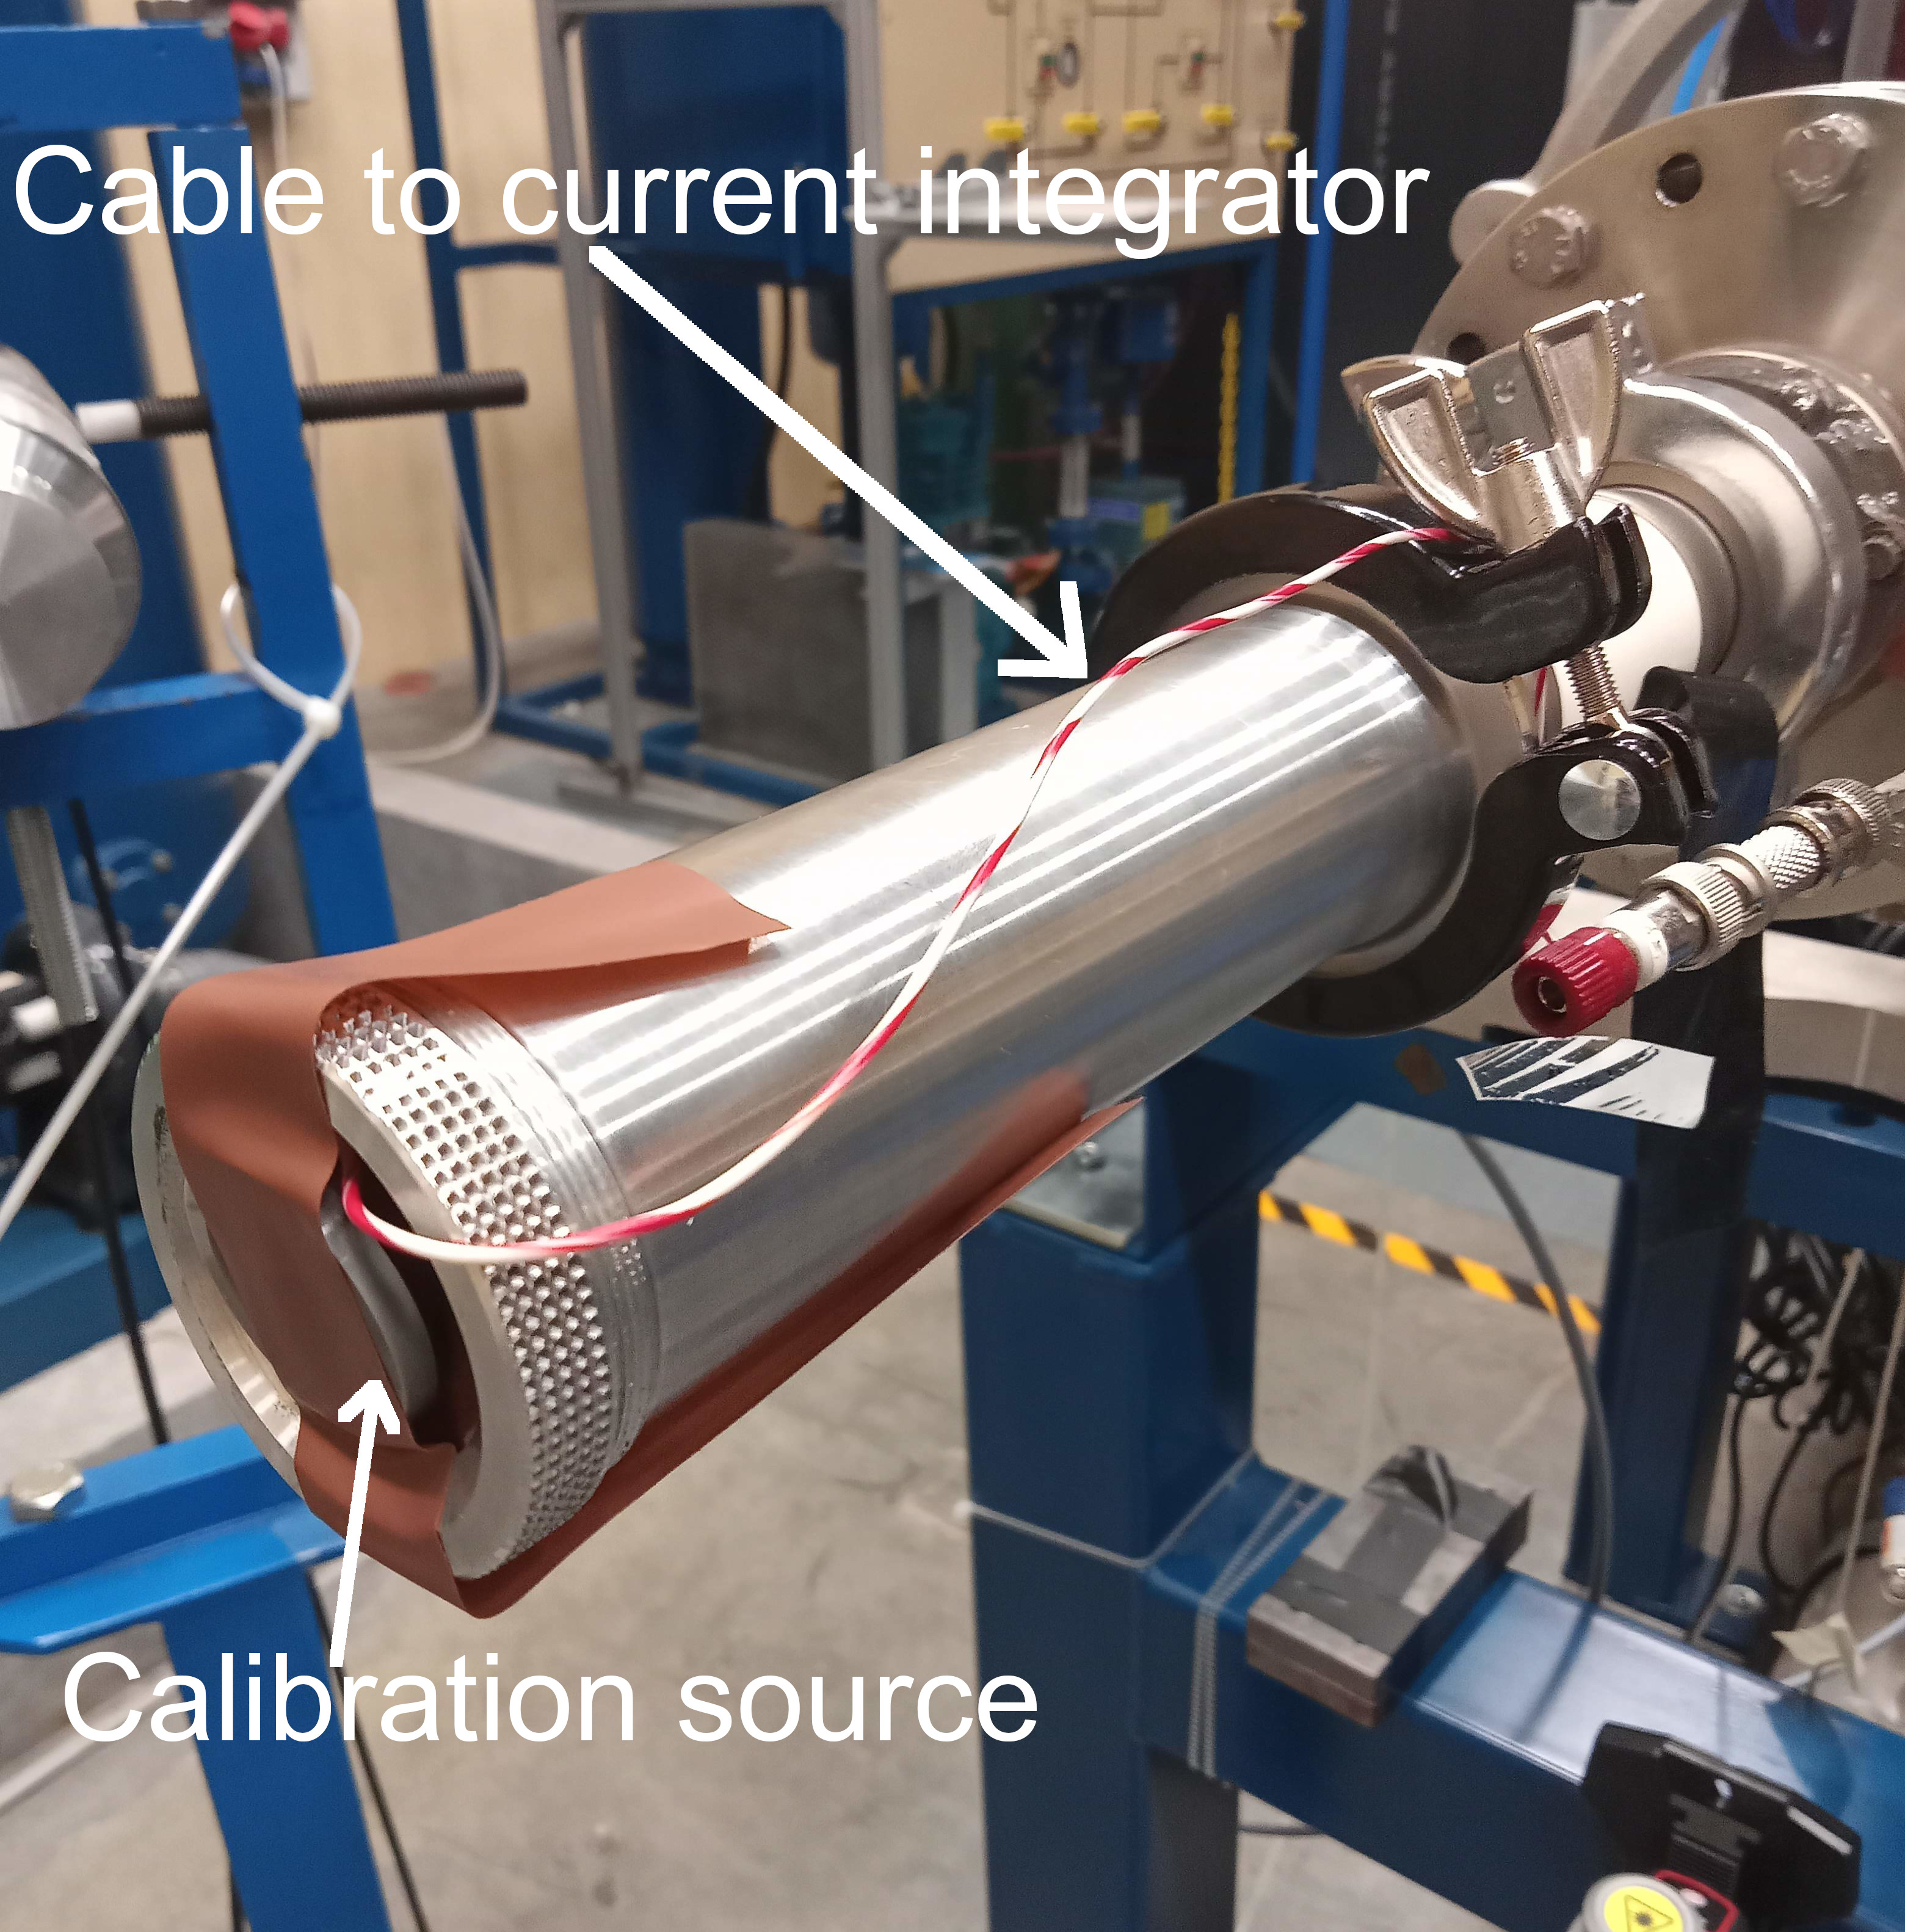
\includegraphics[width=0.5\textwidth]{target_with_calibration.jpg}
	\caption{Target at the end of the neutron line, with a calibration source taped for efficiency calibration measurements.}
	\label{target_photo}
\end{figure}

\subsection{Radiation detectors}
The thick target yield (number of \an reactions per number of incident alphas) will be measured by using gamma detectors, while the \an neutron spectra will be done via time of flight measurements with a neutron detector.
\\

·Drawing with distances and angles of all relevant detectors.\\

\begin{table}[H]	%Tabla con distancias y ángulos de detectores
\centering
\begin{tabular}[c]{>{\bfseries}l||c|c}
	Detector		&Distances\tablefootnote{Detectors were moved in order to get measurements at different distances.} (\unit{\cm})& Angle\\ \hline
	\textbf{MONSTER}	&\num{100}, \num{200}			&\qty{60}{\degree}	\\ \hline
	\textbf{LaBr1}		&\num{20}, \num{10}, \num{30}		&\qty{150}{\degree}	\\ \hline
	\textbf{LaBr2}		&\num{20}, \num{30}			&\qty{210}{\degree}	\\ \hline
\end{tabular}
\caption{Angles and distances of detectors.}
\label{distances_angles_table}
\end{table}

\subsubsection{LaBr}
To measure gammas, we use two LaBr\textsubscript{3} (lanthanum bromide) detectors, which we refer to as "LaBr1" and "LaBr2".
They are inorganic scitillators, meaning they produce light when hit by ionizing radiation.
This can be used to detect gamma rays by the following process:

When a gamma ray hits the material, it gives all of its energy via the photoelectric effect, or part of it through Compton scattering; to an electron in the medium.
This electron travels the scintillator, losing energy by exciting atoms.
When those excited states decay, they emit a \textit{scintillating} light, to which the material is transparent.

This \textit{scintillating} light is directed to a photocathode, where it emits electrons via the photoelectric effect.
These \textit{photo-electrons} are multiplied in a \textit{photomultiplier tube} (PMT), and finally turned into an electric pulse, which is registered as a detection.

Because proportionality is maintained in each of those conversions, we get a spectroscopic response, where more energetic gammas generate proportionately bigger pulses.
\\

To calculate the detectors' efficiency to \qty{511}{\keV} gammas, we use a \Na source that we stick on the target, at the end of the neutron line.
By fitting the resulting peak to a gaussian, we get the number of detected photons per second.
We then divide by the total number of emmited photons (given the source's activity) to get the efficiency.
\begin{equation}
	\text{detector efficiency} = \frac{\text{counts per second}}{\text{total source emissions}}
\end{equation}

\begin{figure}[H]
	\centering
	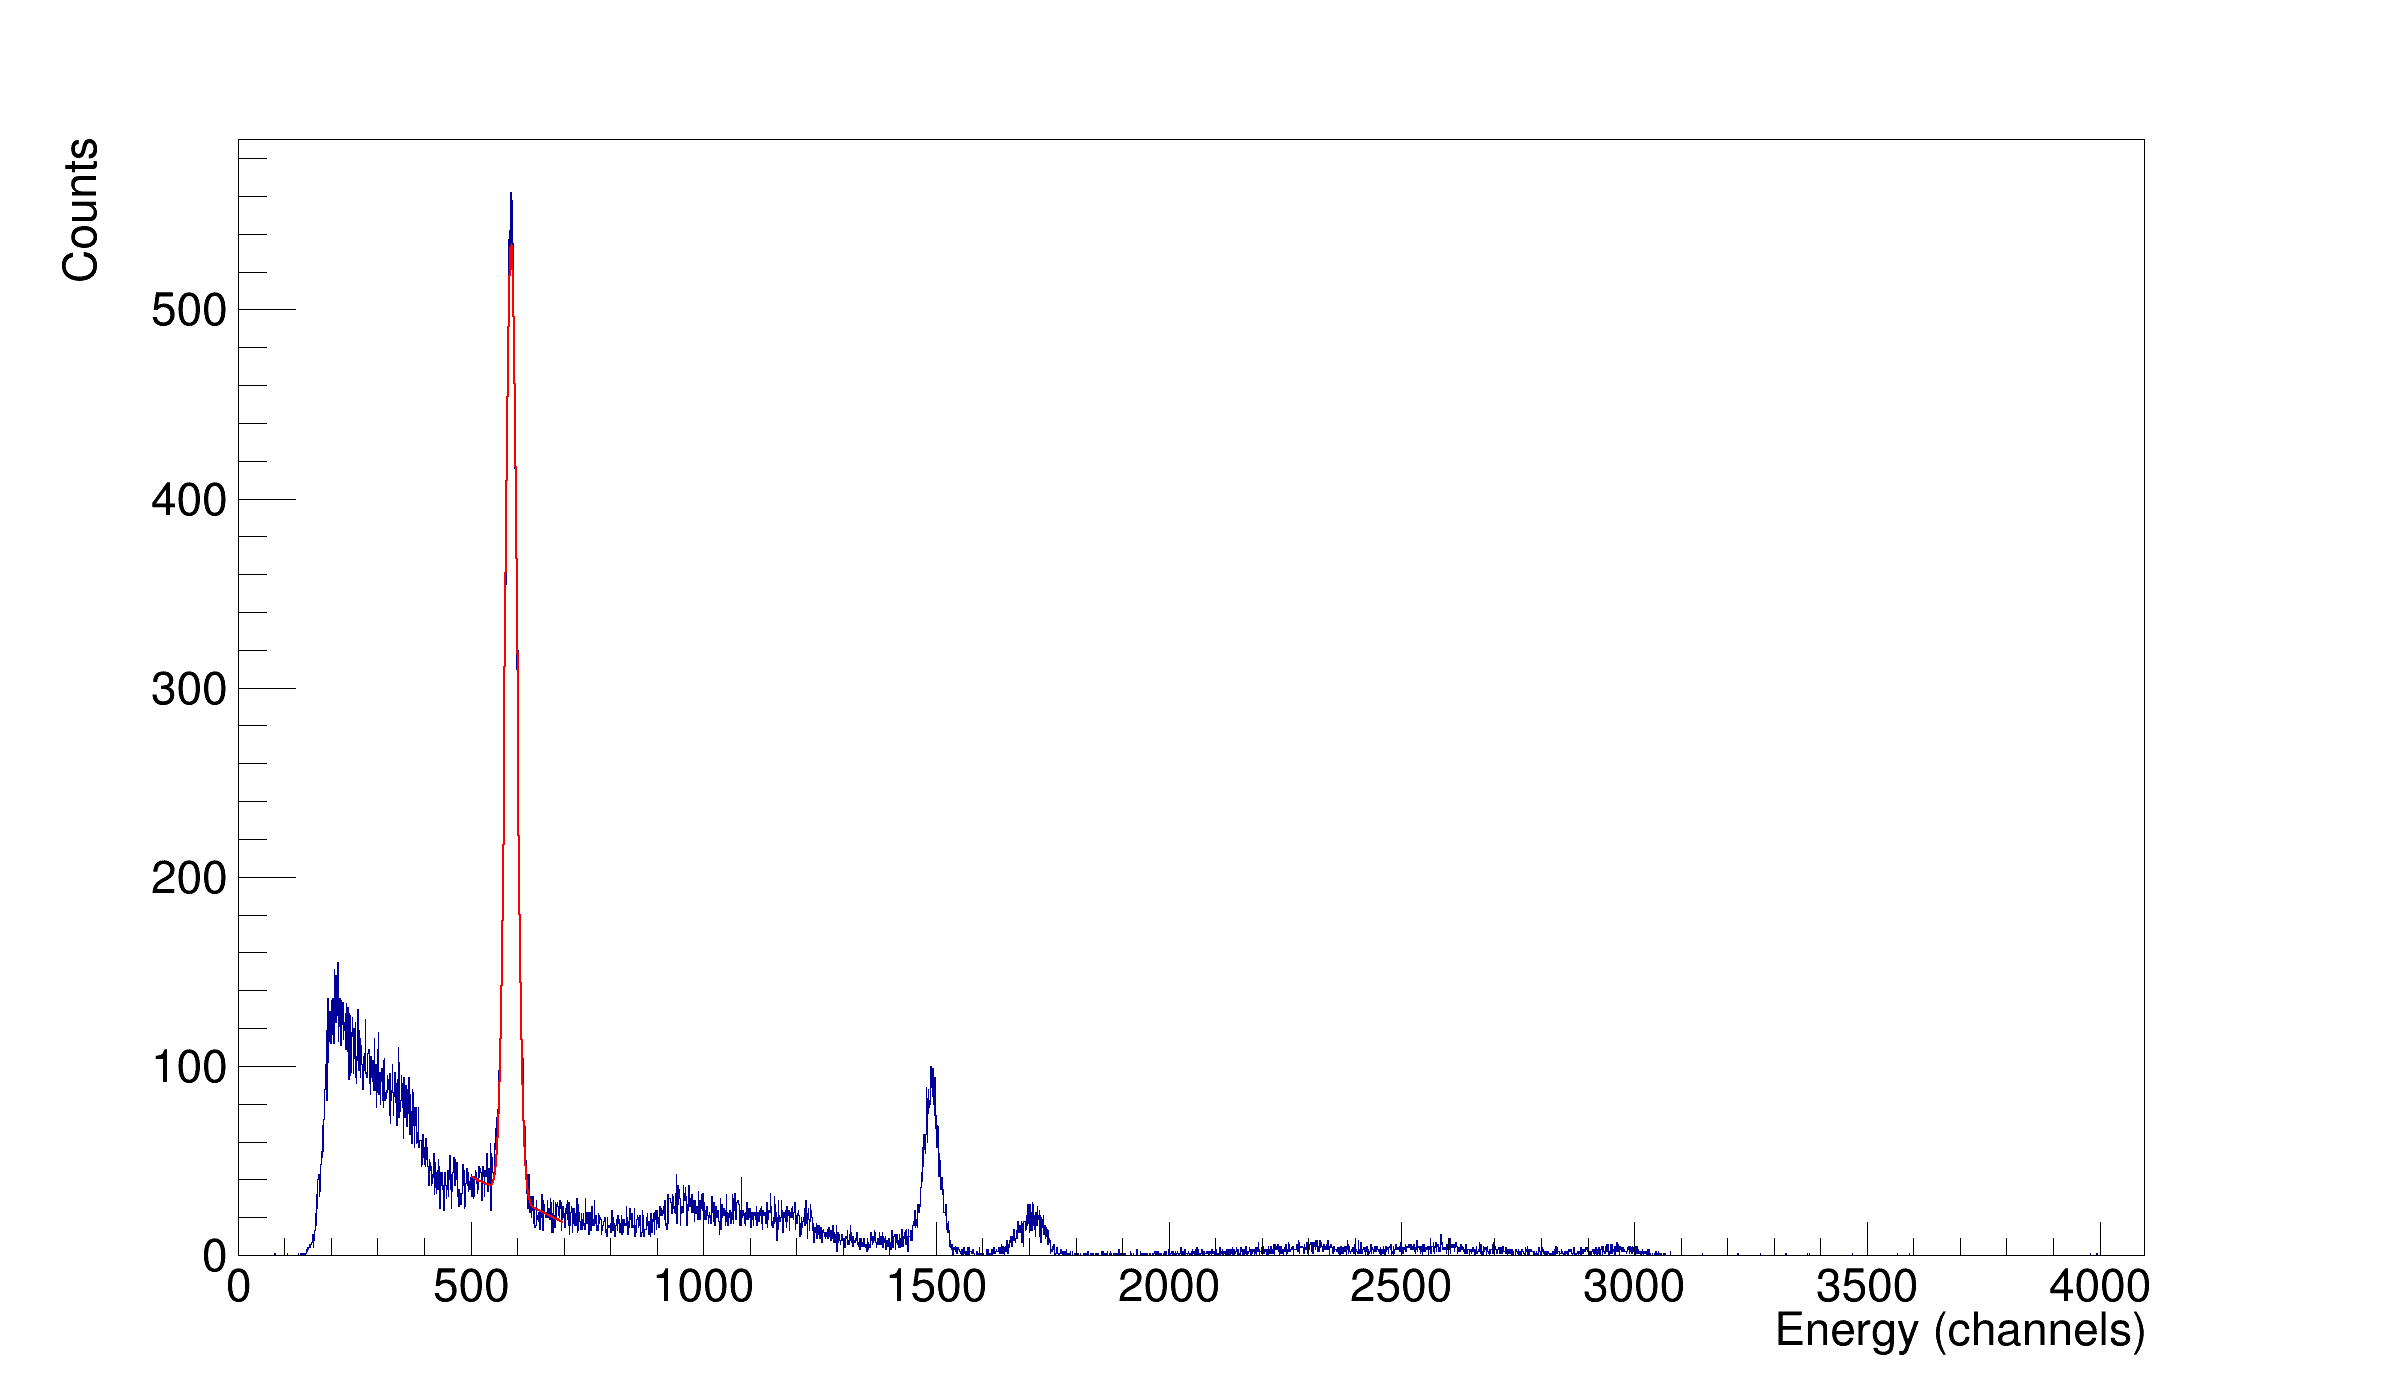
\includegraphics[width=\textwidth]{labr_na22_calibration.png}
	\caption{LaBr1 response to \Na calibration source. In red is the fitting of the \qty{511}{\keV} peak to a gaussian plus a linear background.}
	\label{labr_na22_calibration}
\end{figure}

\begin{figure}[H]
	\centering
	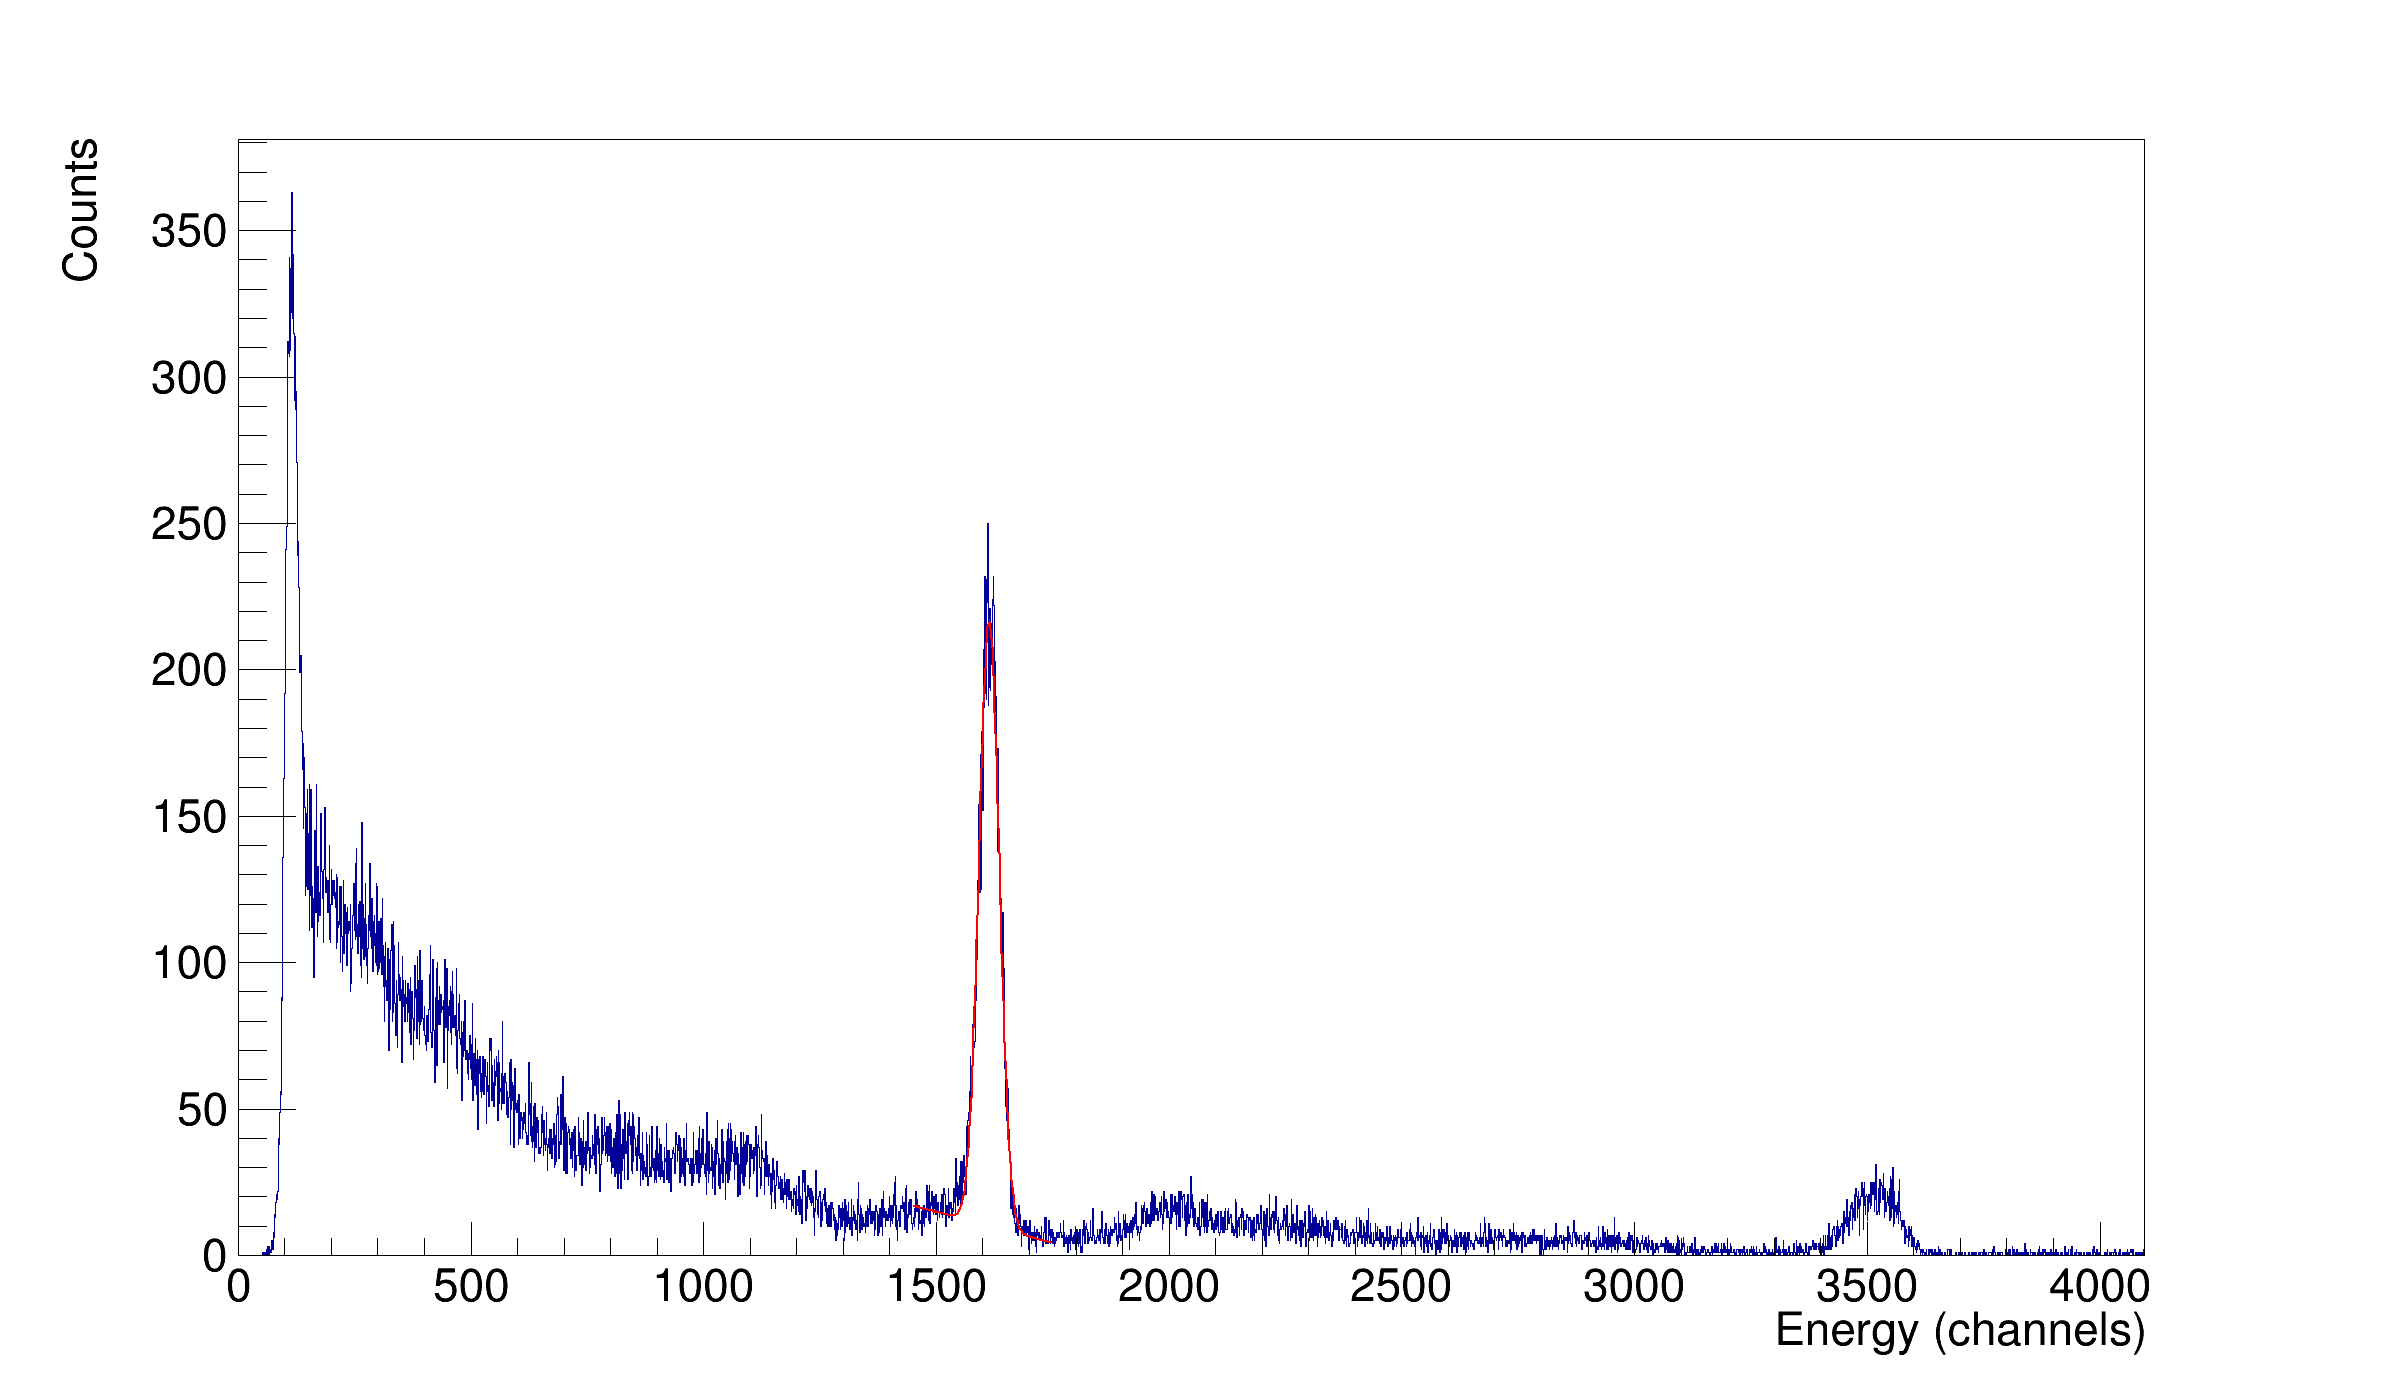
\includegraphics[width=\textwidth]{labr_cs137_calibration.png}
	\caption{LaBr1 response to \textsuperscript{137}Cs calibration source.}
	\label{labr_cs137_calibration}
\end{figure}

\begin{figure}[H]
	\centering
	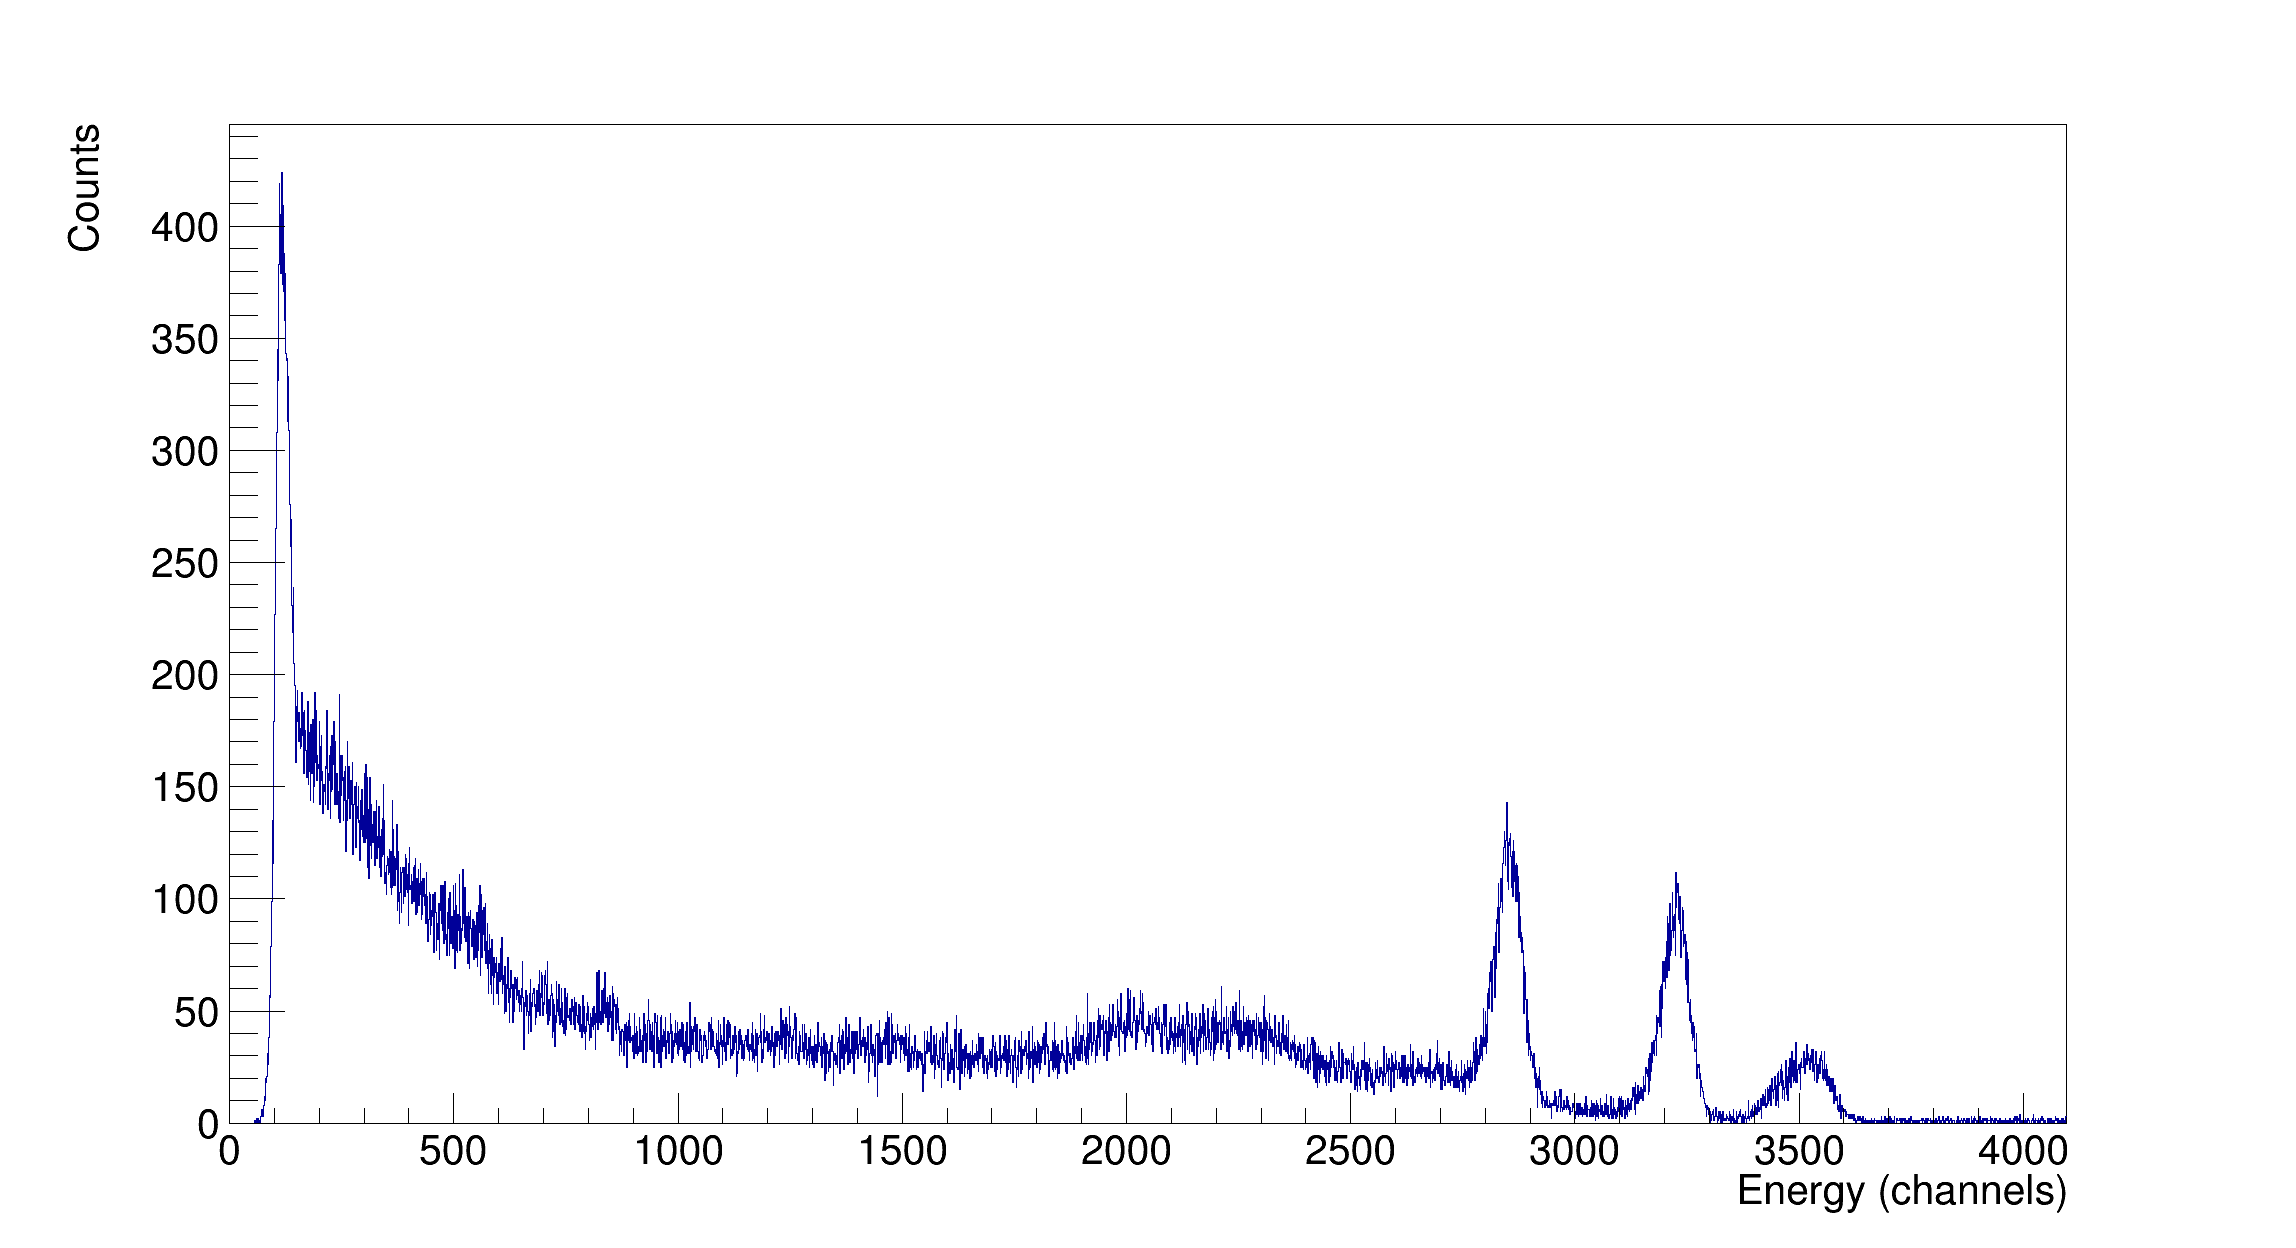
\includegraphics[width=\textwidth]{labr_co60_calibration.png}
	\caption{LaBr1 response to \textsuperscript{60}Co calibration source.}
	\label{labr_co60_calibration}
\end{figure}

\subsubsection{MONSTER}
To measure the time of flight of neutrons produced by \an reactions, we use MONSTER, a liquid organic scintillator.
Two smaller, liquid organic TADEO scintillators were also used, but their data has not been analyzed due to their poorer efficiency.
\\

Their operating principle is the similar to that of inorganic scintillators described before, except that the excited stated that emit the \textit{scintillating} light are molecular in nature, not atomical.
Organic scintillators have a higher efficiency for detecting neutrons than inorganic ones, as neutrons excite the material mostly through $\left( \text{n},\text{p}  \right)$ reactions (unlike gamma rays), which have a higher cross-section with Hydrogen atoms.

Because the molecules are being excited by different charged particles, different states are populated and scintillating light is emmited with longer half-lifes.
This means that the resulting electric pulse is wider, which allow us to differentiate between pulses caused by photons and those caused by neutrons.
This is called \textit{pulse shape discrimination}, or PSD.

\begin{figure}[H]
	\centering
	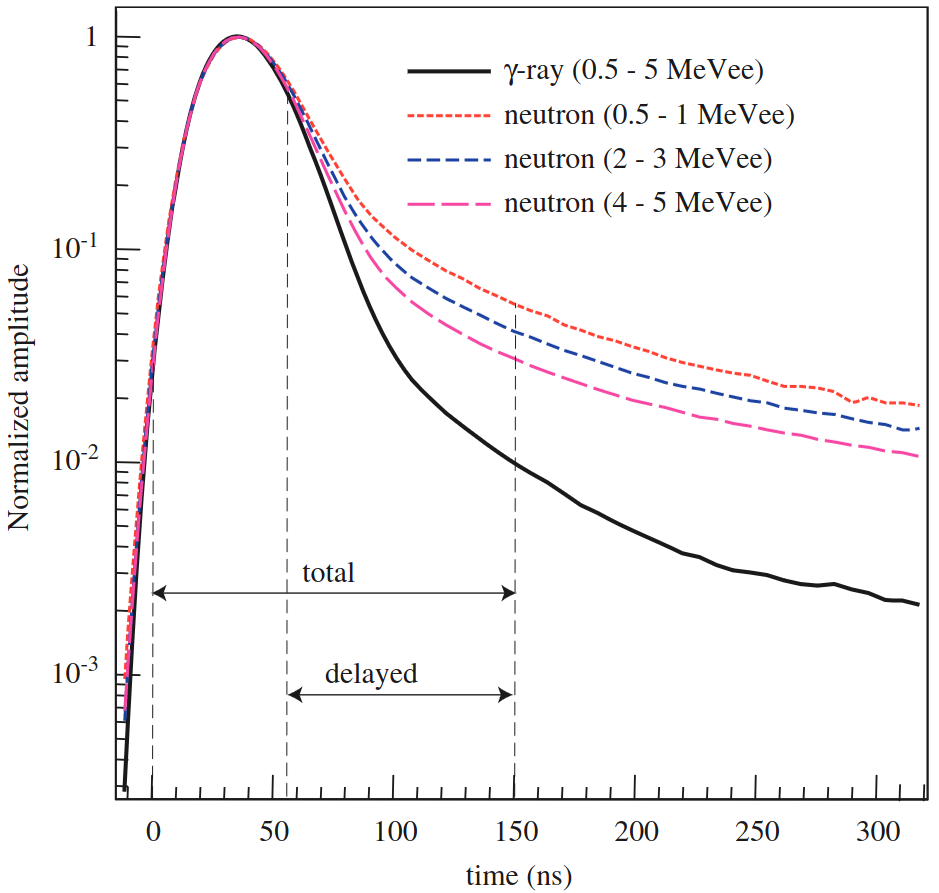
\includegraphics[width=0.35\textwidth]{psd_explanation.png}
	\caption{Illustration od scintillation pulses generated by two different radiation types.}	%TBD:mejor calidad, buscar fuente
	\label{psd_explanation}
\end{figure}

By integrating the charge in a scintillation pulse in two parts, between the initial \textit{fast} rise and the latter \textit{slow} tail, we can calculate a number, PSD:
\begin{equation}
	\text{PSD} = \frac{\text{slow}}{\text{fast}+\text{slow}}	%TBD:check
\end{equation}
that we can use to separate counts corresponding to neutrons from those that correspond to gammas.
At high energies, the \textit{fast} portion saturates, causing the sahpe seen in figure \ref{example_psd}.

\begin{figure}[H]
	\centering
	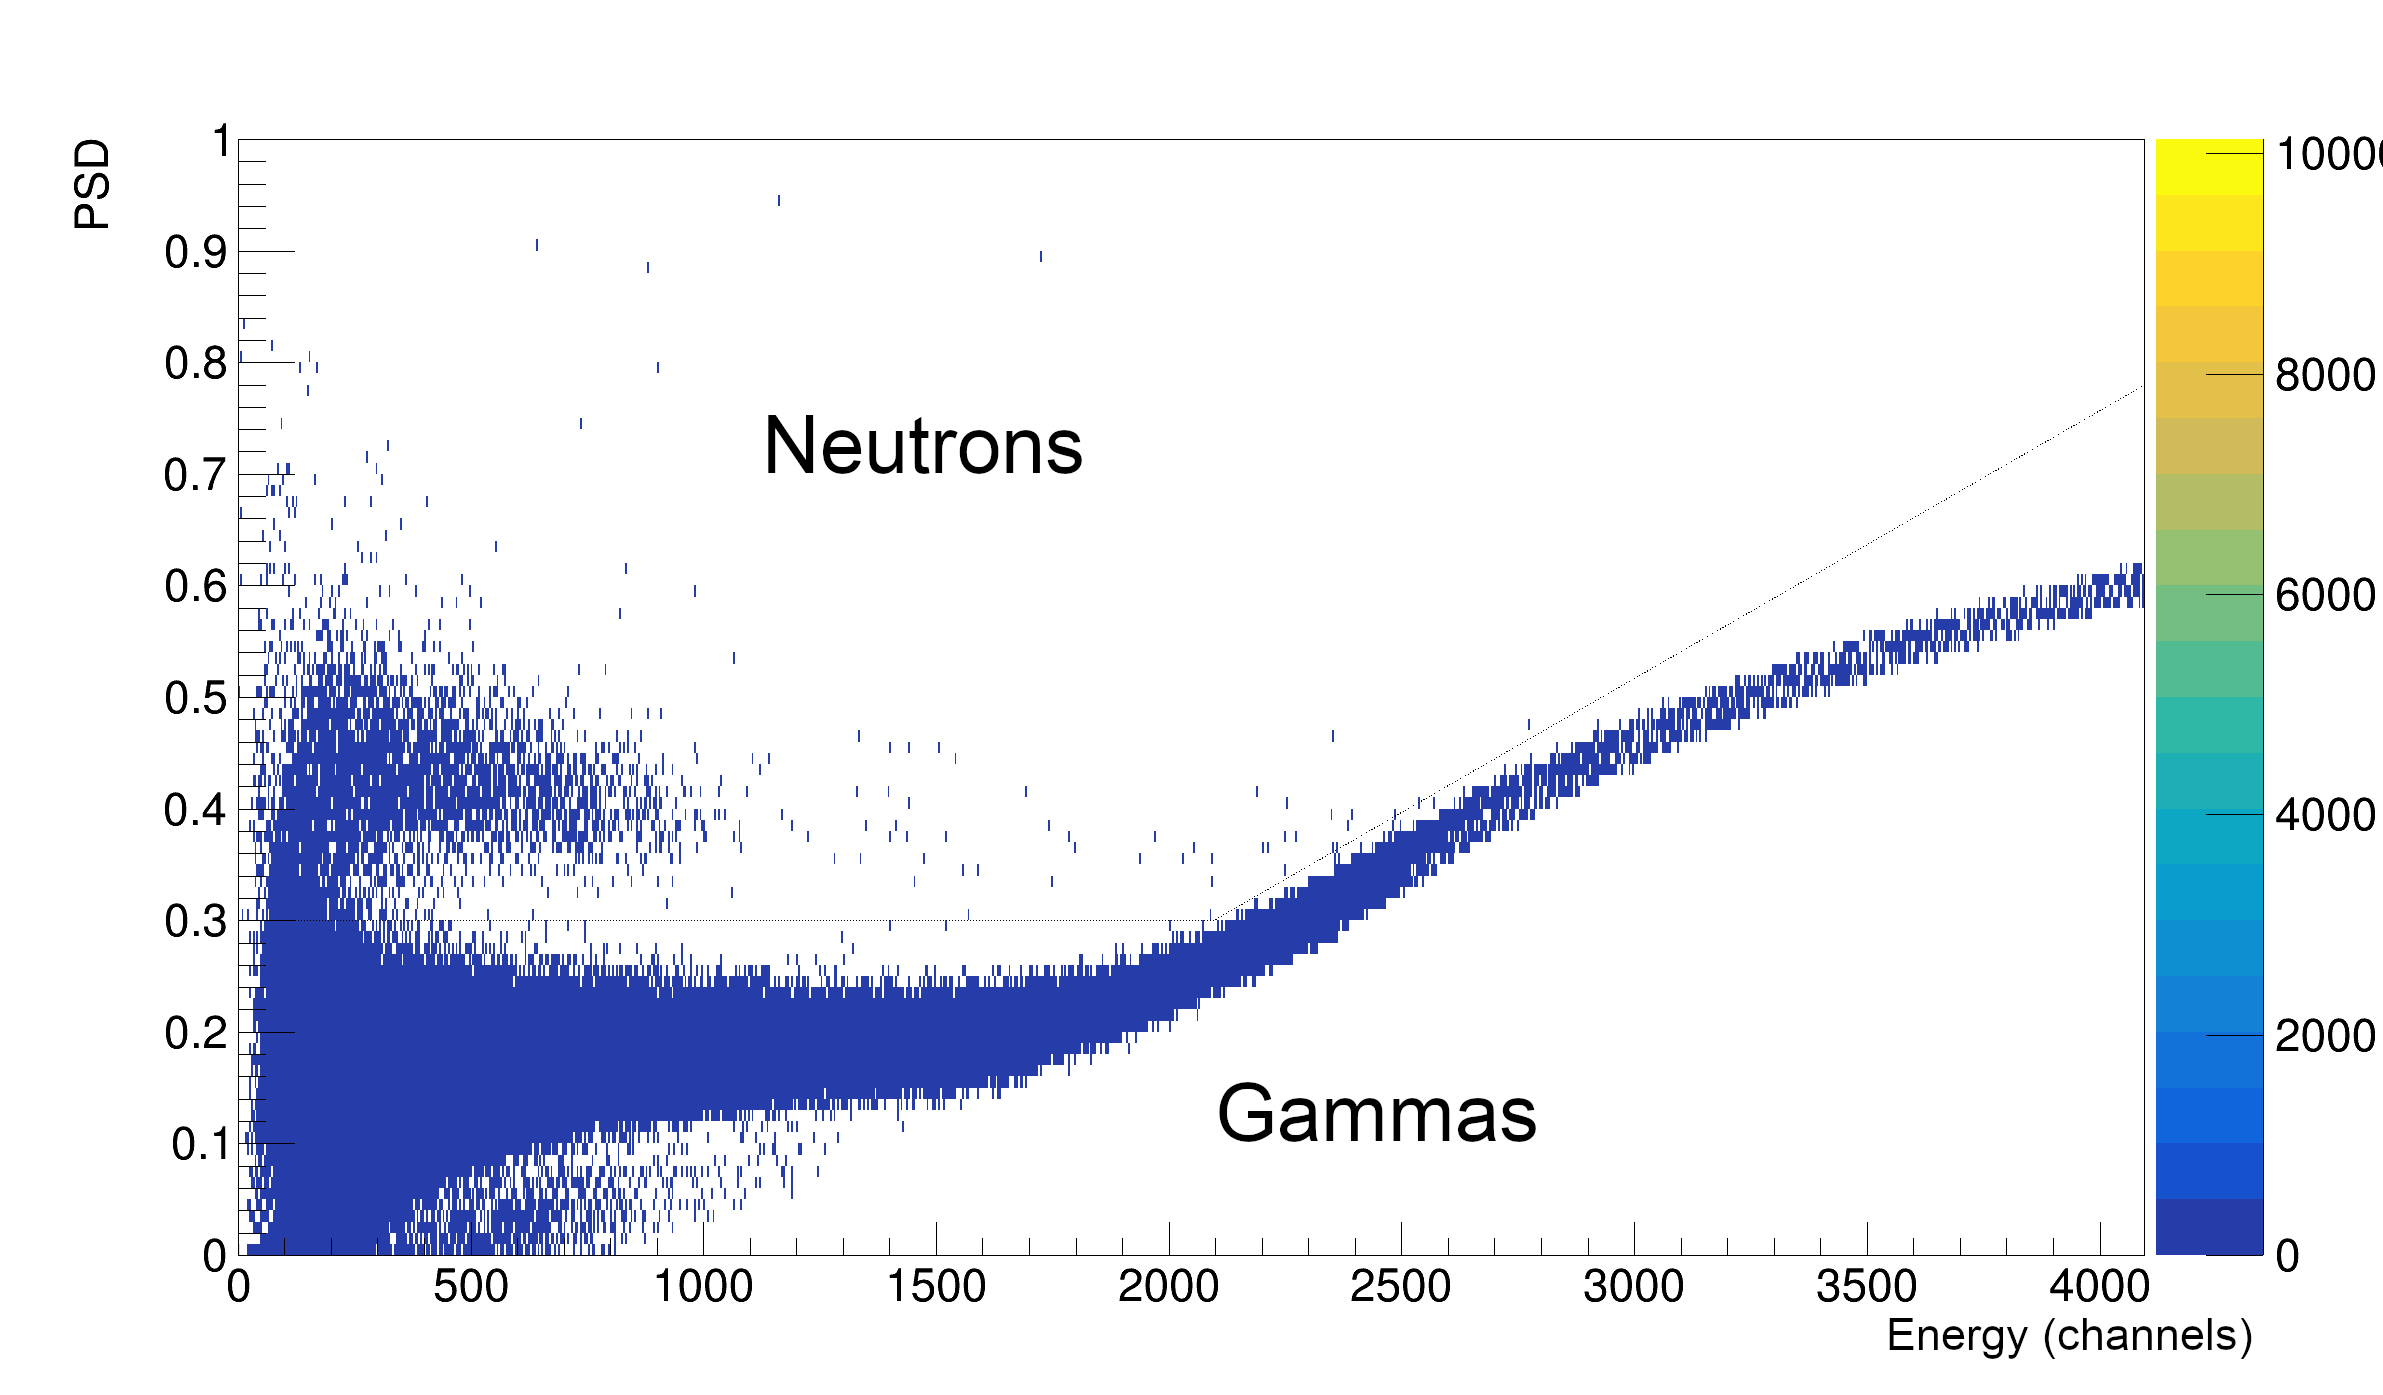
\includegraphics[width=\textwidth]{example_psd.png}
	\caption{2D histogram showing PSD separation between neutrons and gamma rays for a MONSTER measurement.
	The separation line between the two is ahown in black and dotted.}
	\label{example_psd}
\end{figure}

MONSTER's response to photons is different than the lanthanum bromide detectors.
Because it is organic, the cross-section for the photoelectric effect is much smaller; and so photopeaks are not visible, only the Compton continuum is.

\begin{figure}[H]
	\centering
	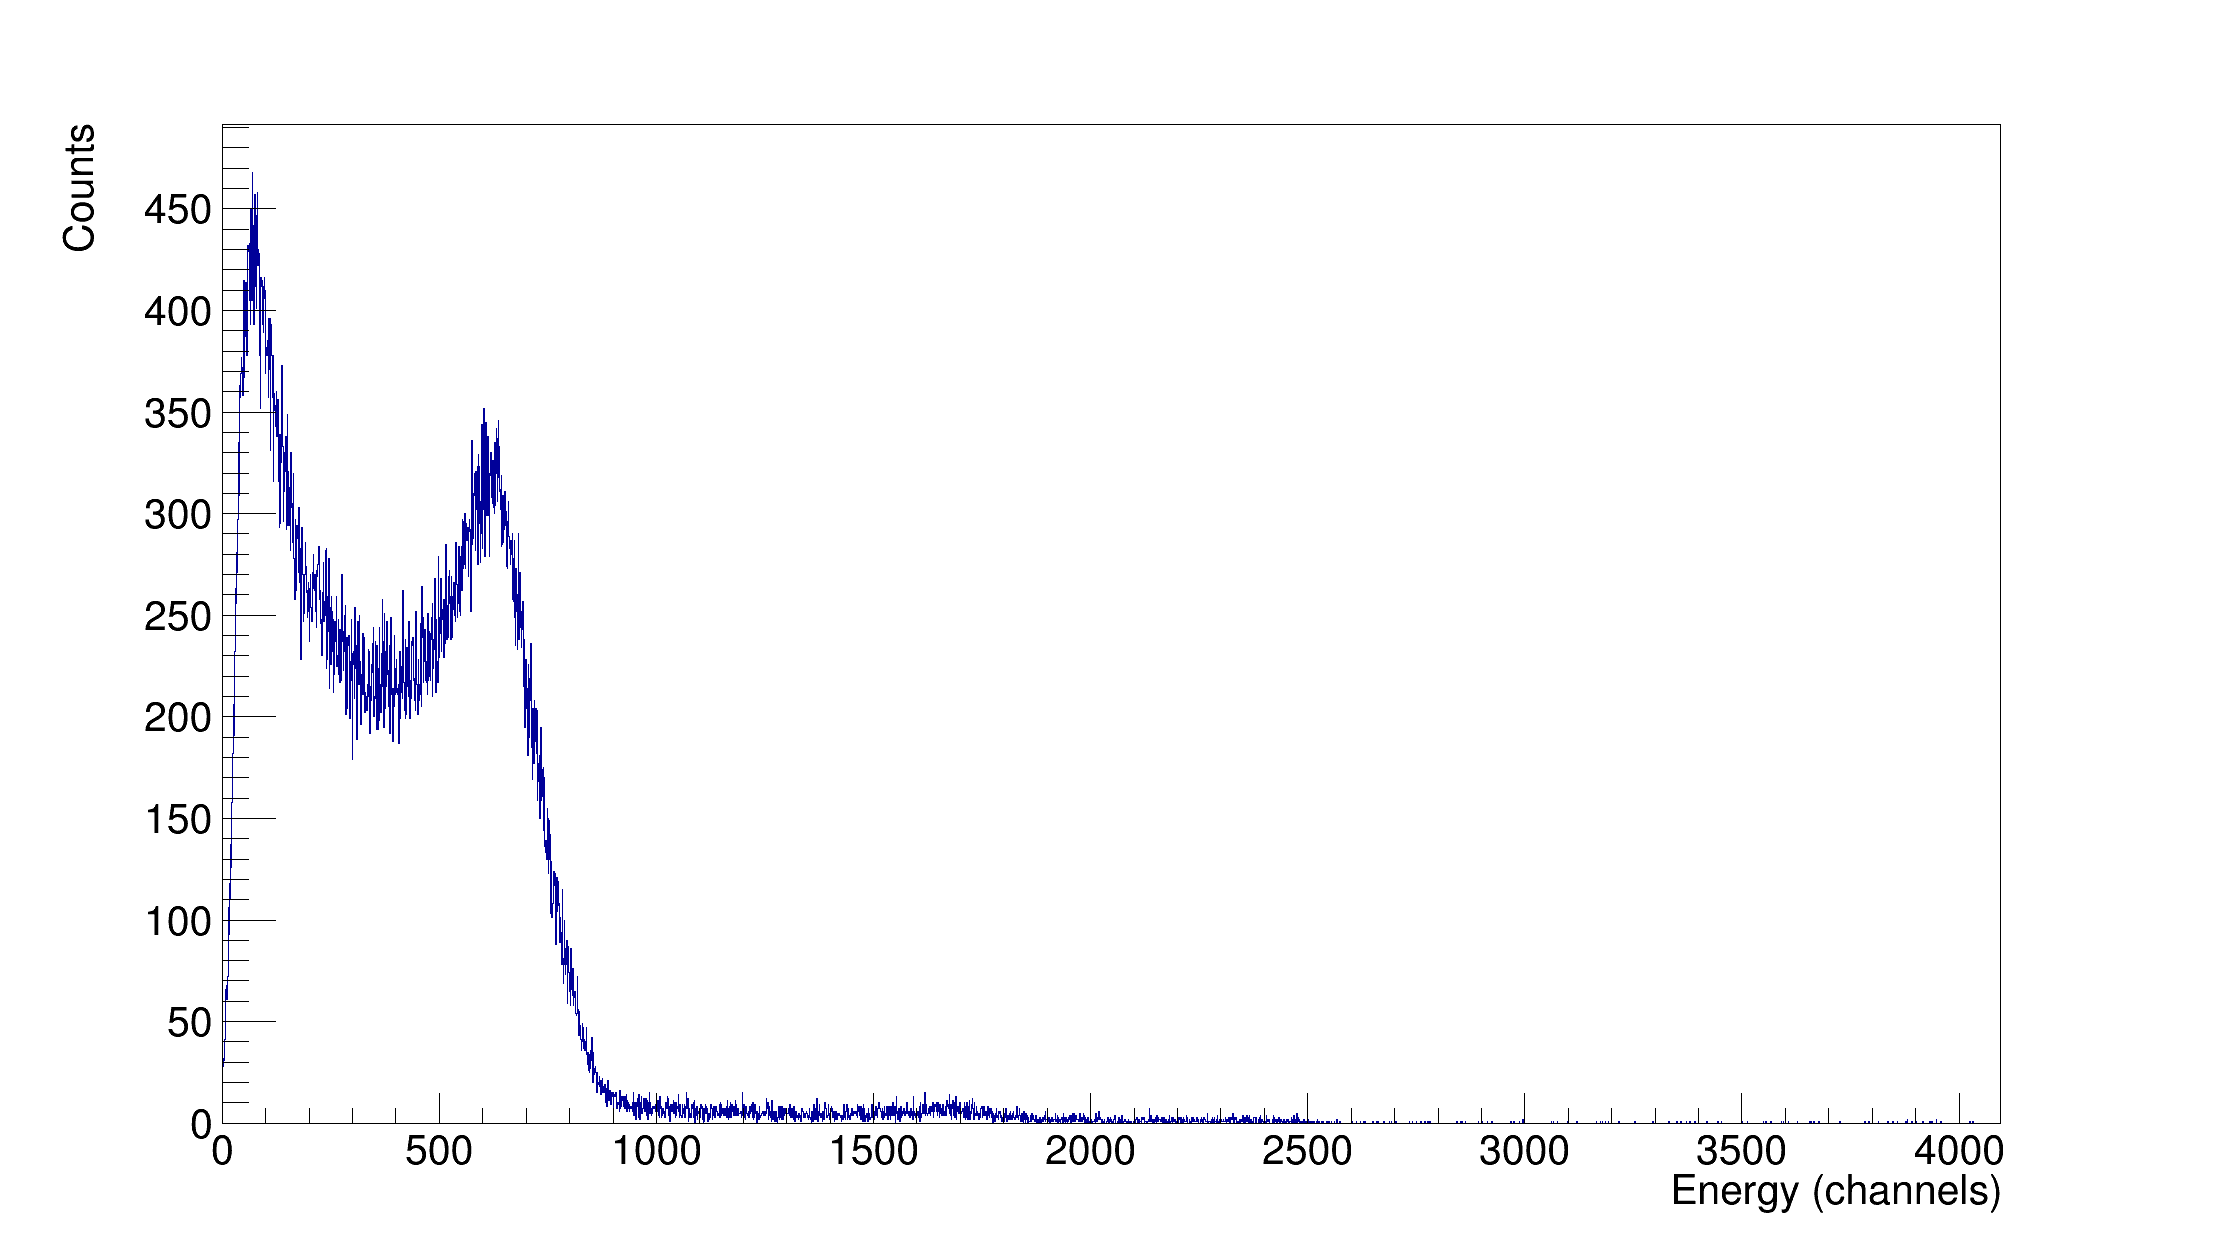
\includegraphics[width=\textwidth]{monster_cs_calibration.png}
	\caption{MONSTER response to \textsuperscript{137}Cs calibration source.}
	\label{monster_cs_calibration}
\end{figure}

\begin{figure}[H]
	\centering
	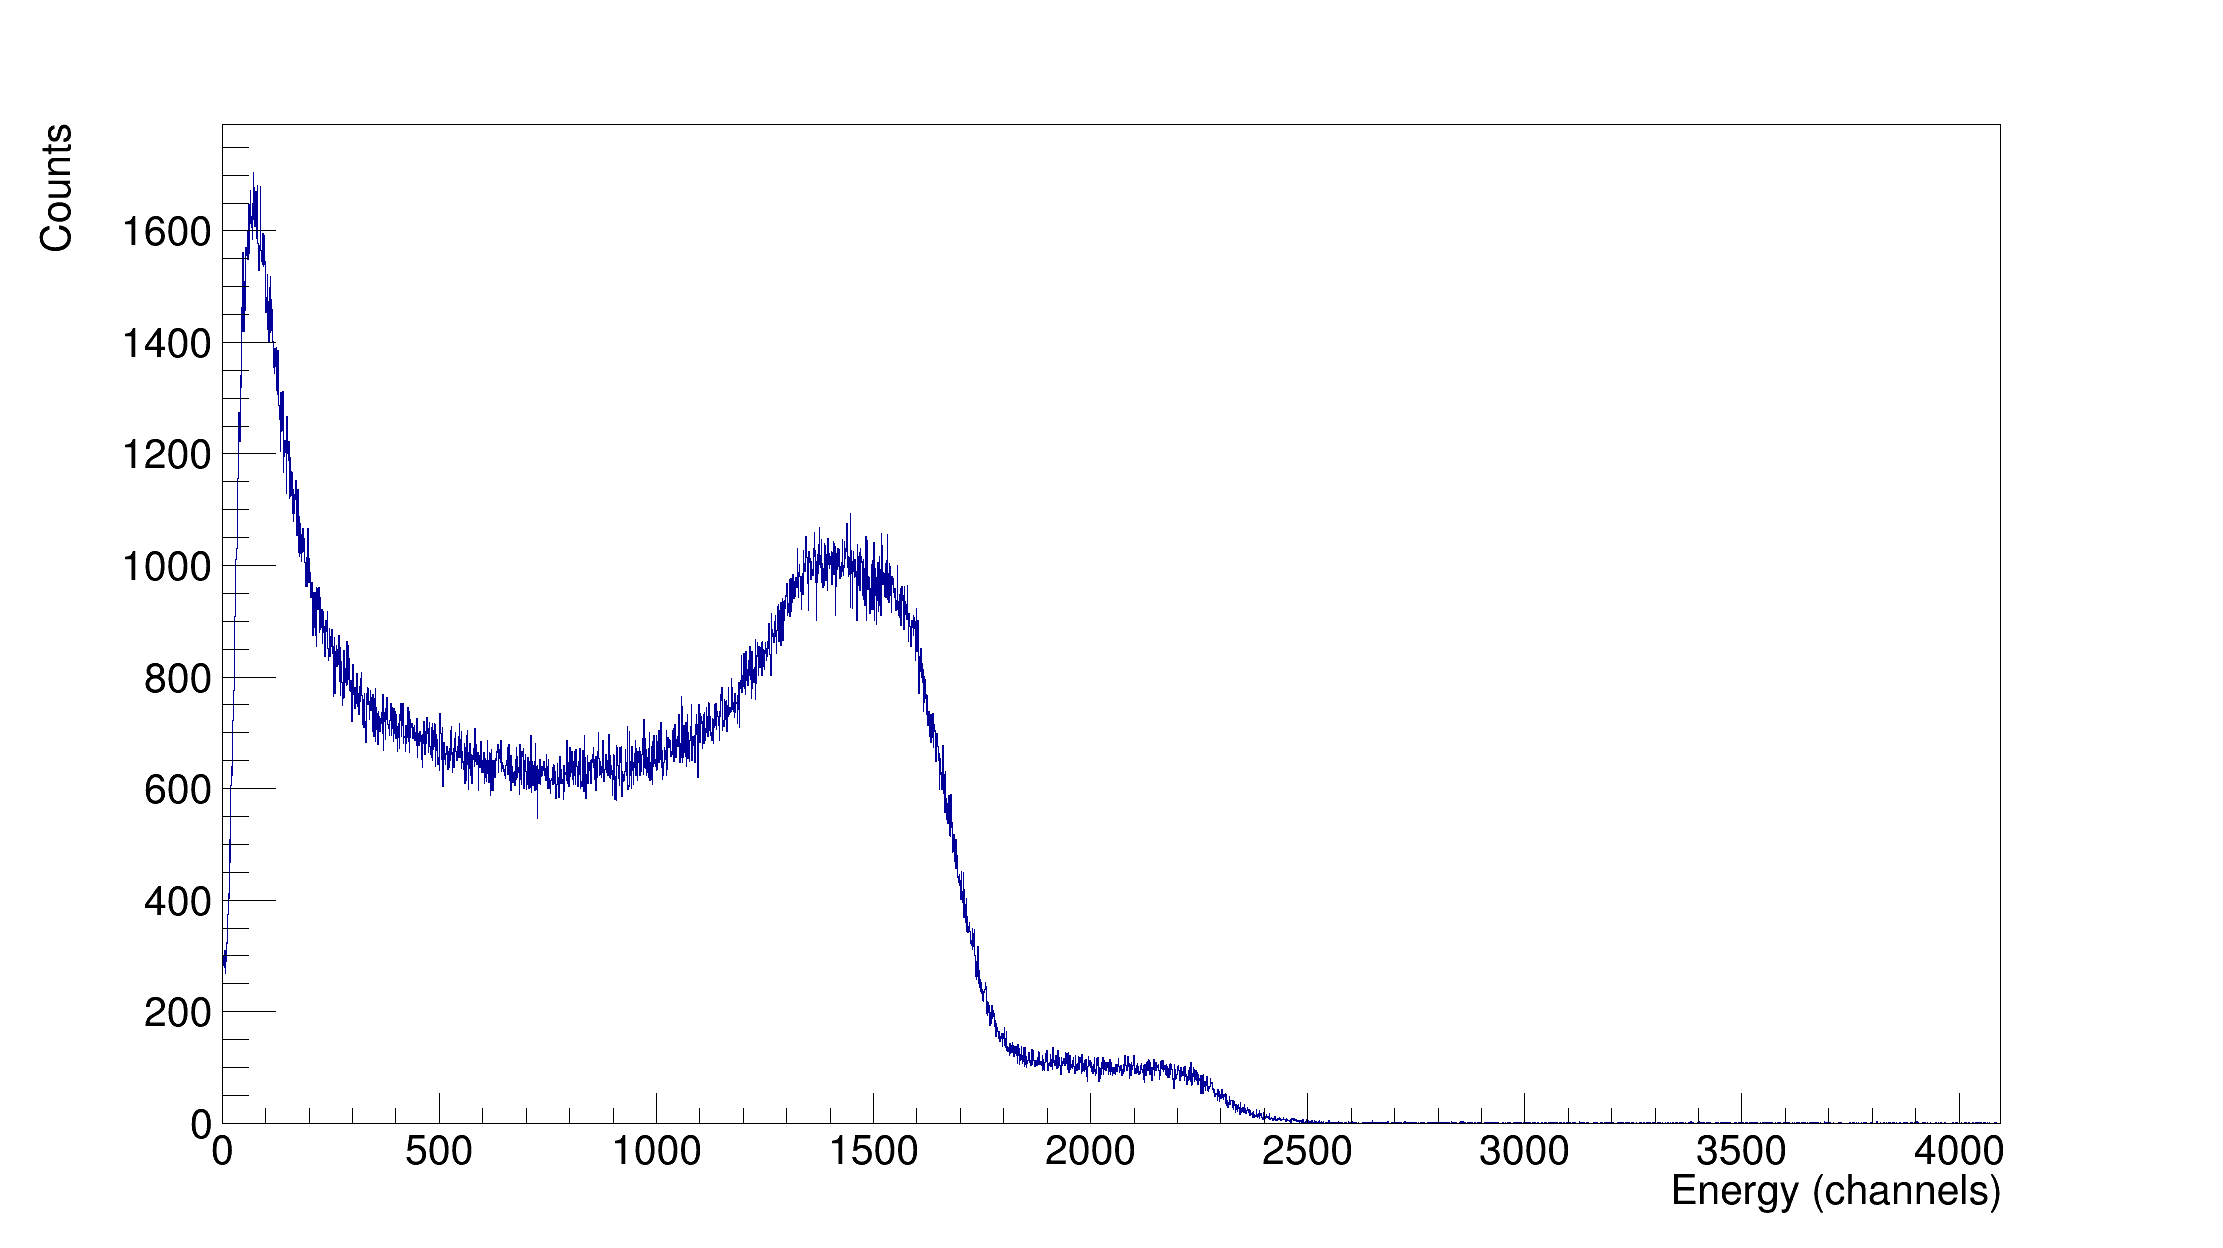
\includegraphics[width=\textwidth]{monster_co_calibration.png}
	\caption{MONSTER response to \textsuperscript{60}Co calibration source.}
	\label{monster_co_calibration}
\end{figure}

·We use a theoretical curve to calibrate in efficiency. Show curve.\\

\section{Procedure}
Two different types of experiments are carried out, \textit{activation} ones to measure thick target yield; and \textit{time-of-flight} ones for neutron spectra.

\subsection{Activation measurements}
For the \textit{activation} measurements, the beam is operated in continuous mode, launching a stream of alpha particles of a certain energy, $E_\alpha$.
When the alpha particles hit the target, \an reactions (among others) occur.
Because the target is thick, these reaction will happen at alpha energies equal to or smaller than $E_\alpha$, as the particles lose energy in the target.

The number of \an reactions will be proportional to the number of incident alpha particles, and the proportionality constant is the \textbf{thick target yield}.
\begin{equation}
	\text{thick target yield} = \frac{\text{number of \an reactions}}{\text{number of incident alphas}}
\end{equation}

Each \an reaction creates a \Piso nuclei, with a \qty{2.498}{\minute} half-life.
It decays to \textsuperscript{30}Si by $\beta +$, emitting \qty{511}{\keV} annihilation gamma-rays with an intensity of \num{1.9971}.\cite{nucleardatasheets}

We can thus indirectly measure the number of \an reactions by measuring the number of created \Piso nuclei.
\\

\begin{figure}[H]
	\centering
	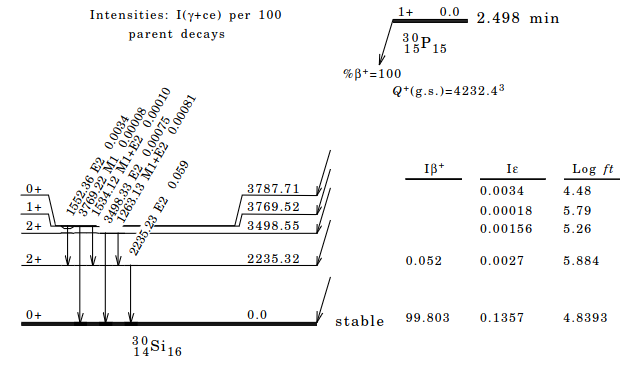
\includegraphics[width=0.7\textwidth]{Piso_decay_scheme.png}
	\caption{\Piso decay scheme.
	From \cite{nucleardatasheets}.}
	\label{Piso_decay_scheme}
\end{figure}

The \Aliso target is irradiated for several \Piso half-lifes, then the current is cut.
The \Piso is then left to decay for several half-lifes.

\begin{figure}[H]
	\centering
	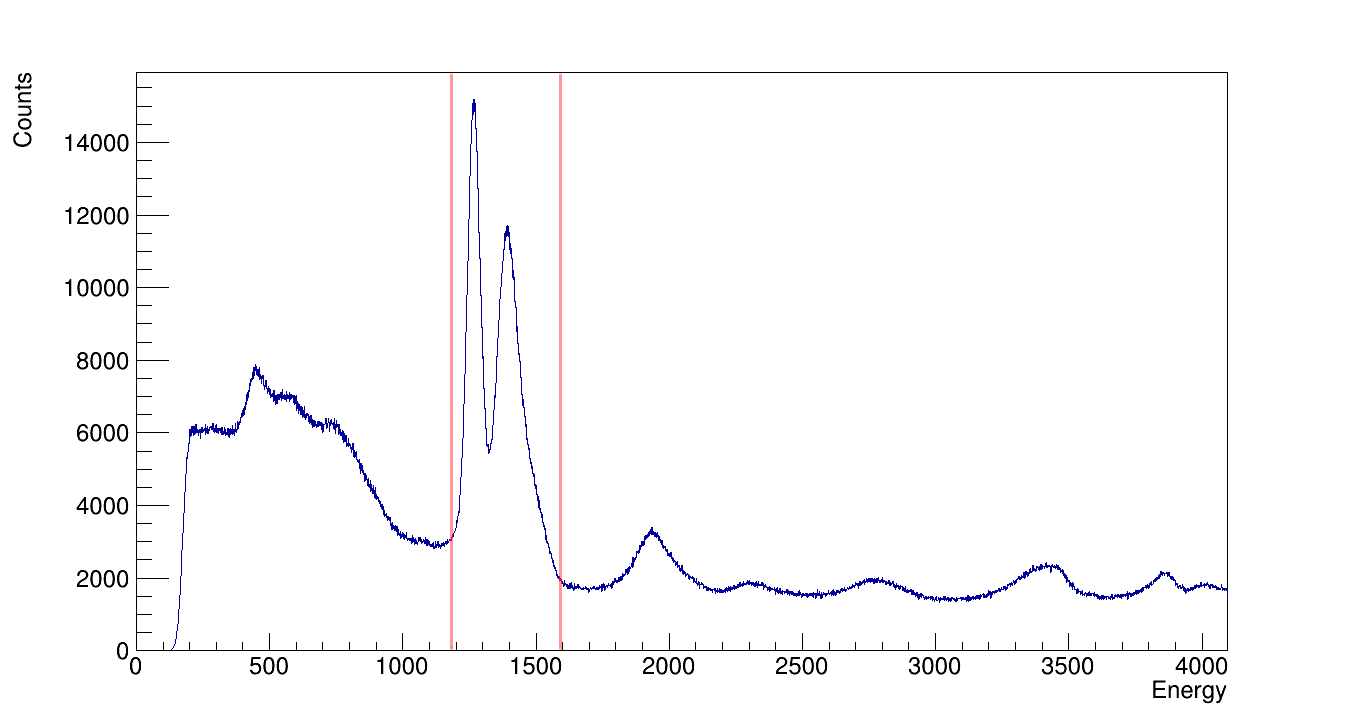
\includegraphics[width=\textwidth]{example_activation_energy_histogram.png}
	\caption{Example activation spectrum.
	The energy window used to generate the time histogram (figure \ref{example_activation_time_histogram}) is shown in red.}
	\label{example_activation_energy_histogram}
\end{figure}

To measure the decay of \Piso nuclei, we look at the \qty{511}{\keV} gamma rays emmited from the target.
Figure \ref{example_activation_energy_histogram} shows the spectrum of one of the LaBr detectors during an activation measurement.
To represent the time histogram (figure \ref{example_activation_time_histogram}), we take only the counts whose energy fall inside the energy window shown in figure \ref{example_activation_energy_histogram}.
The reason there are two peaks, instead of only one, is that the high rate of counts during activation changes the gain of the detectors (figure \ref{example_activation_energytime}), shifting the channel the peak corresponds to.

\begin{figure}[H]
	\centering
	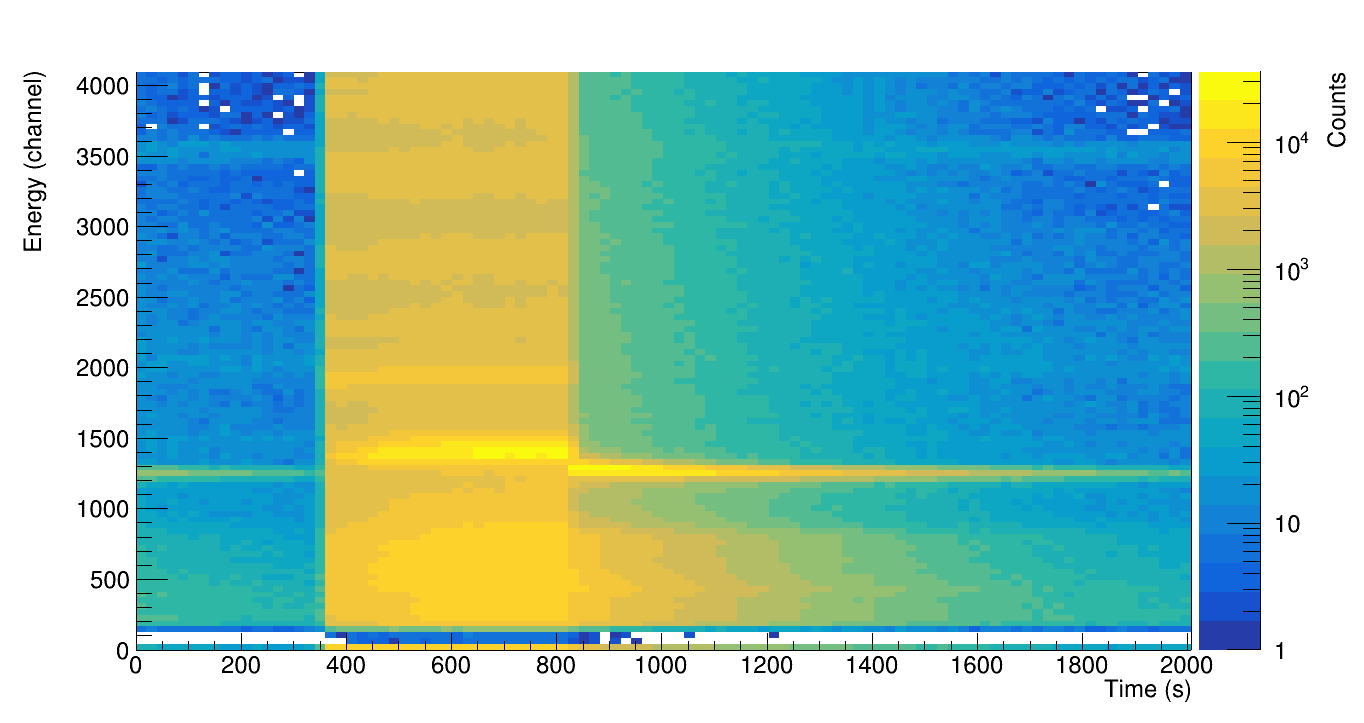
\includegraphics[width=\textwidth]{example_activation_energytime.png}
	\caption{Example activation spectrum over time.
	The change in energy channel for the \qty{511}{\keV} peak is labelled in black.}
	\label{example_activation_energytime}
\end{figure}

\begin{figure}[H]
	\centering
	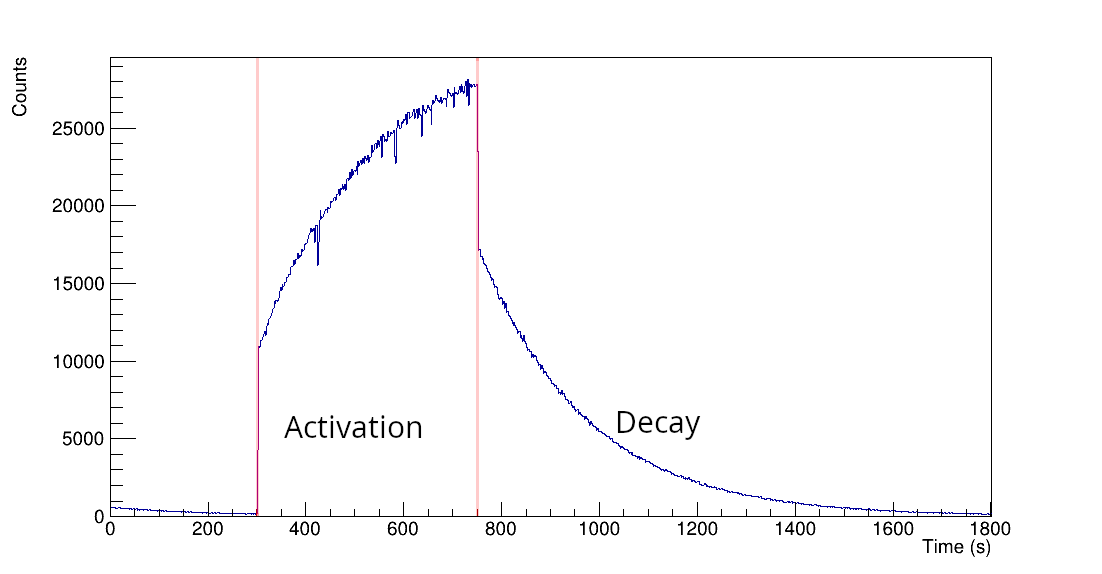
\includegraphics[width=\textwidth]{example_activation_time_histogram.png}
	\caption{Example activation time histogram.
	The activation and decay periods are labeled and separated from the rest of the histogram by red lines.
	The approximate size of the \textit{extra background} caused by the alpha stream is also shown.}
	\label{example_activation_time_histogram}
\end{figure}

The time histogram in figure \ref{example_activation_time_histogram} shows initial counts before the activation starts, corresponding to decay of \Piso from the previous measurement.
When the activation starts, \num{\approx 11000} counts per bin appear very quickly.
These counts go away as soon as the activation period ends.

We call these counts the \textit{extra background}.
They are proportional to the alpha current, and correspond to gamma rays created by reactions other than \an.
They can also be seen in figure \ref{example_activation_energytime}, as the large number of counts appearing during activation well outside of the \qty{511}{\keV} peak.
They affect the histogram because, even if the emitted gammas are outside of the energy window, their Compton continuum still falls inside.

After activation ends, we get the counts corresponding to the decay of \Piso nuclei.

\subsection{Time of flight measurements}
For the time of flight measurements, the beam is operated in pulsed mode.
This means that, ideally, alphas arrive in groups, all at the same time, with a certain frequency.	%TBD: especificar anchura, frecuencia.
Because of that, all of the \an reactions occur and all of the neutrons are produced at the same time.

Each time the accelerator's chopper/buncher acts, an electric signal is emitted.	%TBD:chopper o buncher?
This signal is what we use to time every detection in relation to a pulse.
It doesn't correspond to when the pulse arrives at the target, but all of them arrive with the same delay with respect to it.
\\

Both gammas and neutrons are produced at the same time by the \an reactions.	%TBD:mirar tiempo de producción de gammas
Gamma rays move at the speed of light, and thus all arrive at the detector $d/c$ time later, with $d$ the distance to the target.
This is called the \textit{gamma flash}.

Neutrons, however, have different speeds depending on their energy, and arrive at the detector different amounts of time later.
This time is called the \textit{time-of-flight}, or ToF; and from it we can get the energy of the produced neutrons as $E=\frac{1}{2} m_\text{n} \left( \frac{d}{\text{ToF}} \right)^2$, with $m_\text{n}$ the mass of a neutron.
\\

In practice, alphas do not arrive all at the same time: the pulses always have a certain width.
Generally, the time the particles hit the target can be approximated by a gaussian distribution.
This introduces uncertainty in the ToF, and thus energy, measurements.

The width and shape of the alpha pulses will be the same as that of the gamma flash.
This is because the photons travel all at the same speed, and because we assume that the production of gammas is the same for all alphas in a pulse.
\\

\begin{figure}[H]
	\centering
	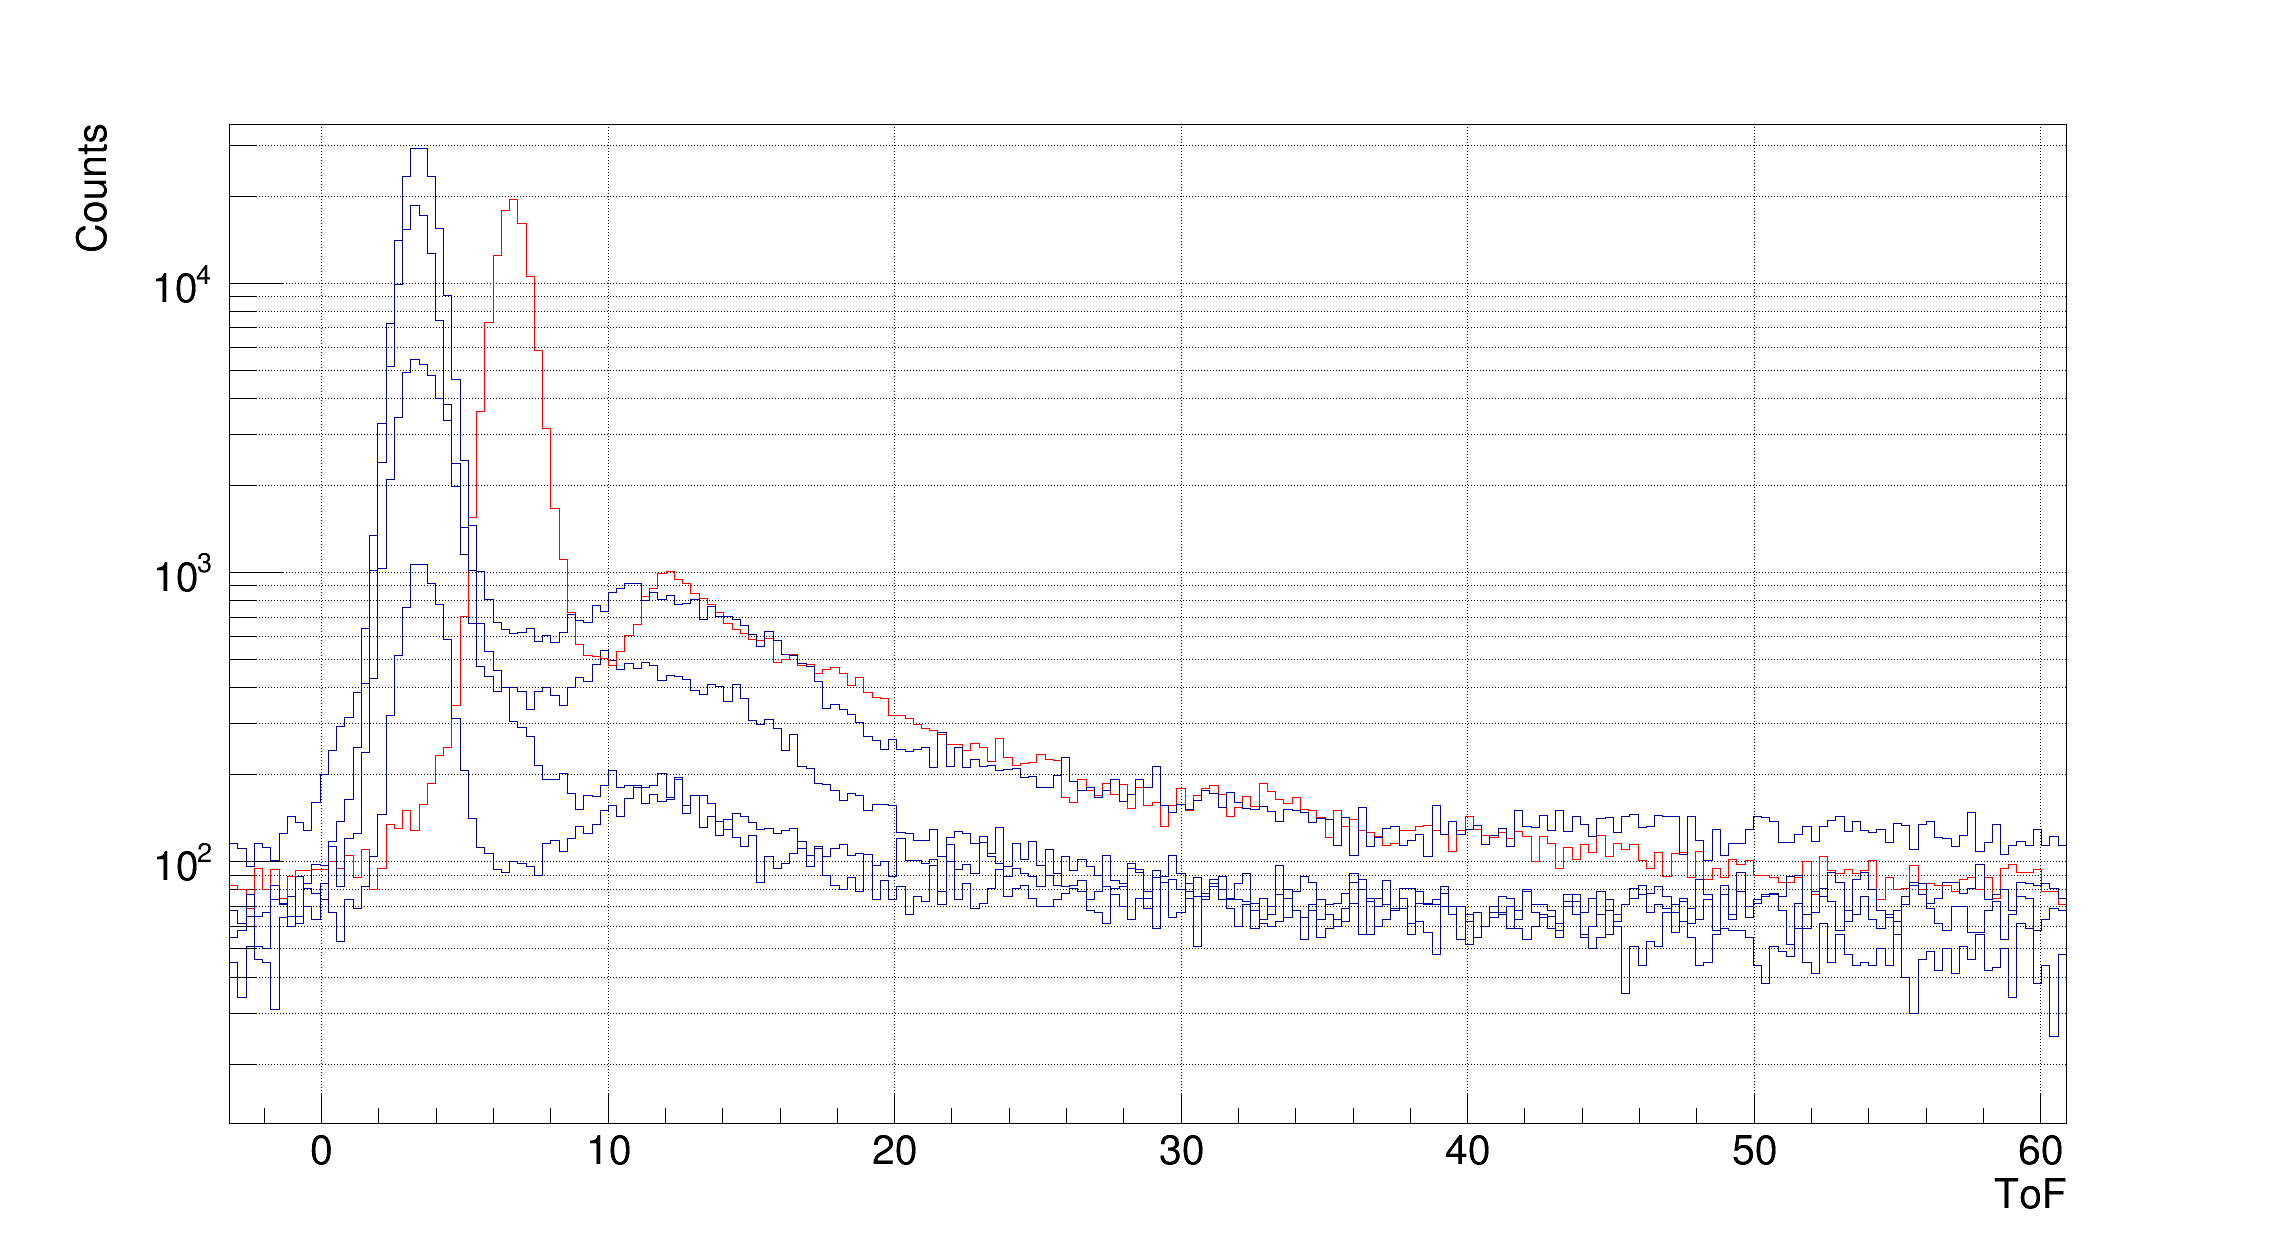
\includegraphics[width=\textwidth]{uneven_gflash.png}
	\caption{Superposition of all histograms of gamma flashes.
	In red is a measurement taken at double the distance than the others.
	It is displaced to the right because of the longer time photons take to travel the distance to the detector.}
	\label{uneven_gflash}
\end{figure}

We can see that the pulses are not symmetrical: they have long tails; and some of them, several peaks.
This means we cannot treat them as gaussians and the introduced error in ToF as their standard deviation.

·Show example ToF plot with and without PSD.\\

\chapter{Measurements, analysis and results}

\section{Activation}
Activation measurements were carried out in two sessions of two consecutive days, in February and April.
Table \ref{activation_measurements_table} summarises the different measurement conditions.

Because detectors were unmounted in between both sessions, calibration measurements with \Na to determine detector efficiency (for activation measurements) were done for each detector configuration.

\begin{table}[H]	%Tabla con datos de las medidas de activación
\centering
\begin{tabular}[c]{>{\bfseries}r||c|c|c|c}
	N & Energy (\unit{\keV}) & Current (\unit{\nano\A}) & Activation time (\unit{\s}) & Date\tablefootnote{All took place in 2023.} \\ \hline
	1	&\num{5500}&\num{128}&\num{867}&Feb 22nd\\ \hline
	2	&\num{7000}&\num{101}&\num{981}&Feb 22nd\\ \hline
	3	&\num{8500}&\num{128}&\num{909}&Feb 22nd\\ \hline
	4	&\num{8500}&\num{192}&\num{899}&Feb 23rd\\ \hline
	5	&\num{5500}&\num{123}&\num{605}&Apr 17th\\ \hline
	6	&\num{5500}&\num{312}&\num{599}&Apr 17th\\ \hline
	7	&\num{8250}&\num{193}&\num{452}&Apr 18th\\ \hline
	8	&\num{7000}&\num{216}&\num{466}&Apr 18th\\ \hline
	9	&\num{5500}&\num{151}&\num{451}&Apr 18th\\ \hline
	10	&\num{7500}&\num{183}&\num{448}&Apr 18th\\ \hline
\end{tabular}
\caption{Activation measurements}
\label{activation_measurements_table}
\end{table}

\subsection{Data analysis}
We can describe the number of \Piso nuclei in the target, $N$, using the differential equation:
\begin{equation}
	\ddt{N} = P(t) -\lambda N
	\label{activation_diffeq}
\end{equation}
where $\lambda$ is the decay constant of \Piso and $P(t)$ is the number of \Piso nuclei created (by \an reactions) per unit of time.
$P(t)$ will be proportional to the current of alphas hitting the target.
If expressed in number of alphas per second, the proportionality constant will be the thick target yield of the reaction; the number of \an reactions per incident $\alpha$ particle.
\\

In order to get $P(t)$, we analyze the activity of \Piso nuclei as they decay by $\beta +$, which will be $A = \lambda N$.
We don't measure the activity directly, but rather the activity times $1.99$: the intensity of the \qty{511}{\keV} emission.	%TBD: referencia para intensidad, tipo de decay

To do that, we use the two LaBr scintillators to detect \qty{511}{\keV} gamma rays.
Some counts will be noise, corresponding not to \Piso decays, but to the Compton continuum of other emissions either in the environment or due to other reactions caused by the alphas.

Furthermore, when representing the counts in a histogram, the number shown is dependent on the width of the bins.
This means that, in order to get the activity in decays per second, we must divide the counts shown in a histogram by 1.99 and by the histogram binwidth.
\begin{equation}
	A = \text{\Piso decays per second} = \frac{\text{counts per bin}}{\text{binwidth}\cdot\num{1.99}} - \text{background}
\end{equation}
We use three different methods to get $P(t)$, depending on wether $P(t)$ is considered constant during the activation period or not; and on the part of the histogram being looked at.

\subsubsection{Decay fit}
After the activation period is over, we are left with a certain number of \Piso nuclei that will decay following a radioactive decay law.
For the \textit{decay} fit, we fit this part of the activation histogram to a negative exponential, $A(t) = A\textsubscript{EOA} e^{-\lambda t} + B$ to get the \Piso activity at the end of activation, $A$\textsubscript{EOA}.

The fit also considers a constant background $B$, coming from the environment.
The value of the decay constant $\lambda$ is fixed to that of \Piso, and not determined by the fit.
Thus, the fit returns only two values: the constant background $B$, and the initial activity $A$\textsubscript{EOA}.
\\

We divide $A$\textsubscript{EOA} by $\lambda$ to get the number of \Piso nuclei at the end of activation, $N$\textsubscript{EOA}.
But $N$\textsubscript{EOA} is not the number of \Piso nuclei created by \an reactions, as some decay during the activation period.

\begin{figure}[H]
	\centering
	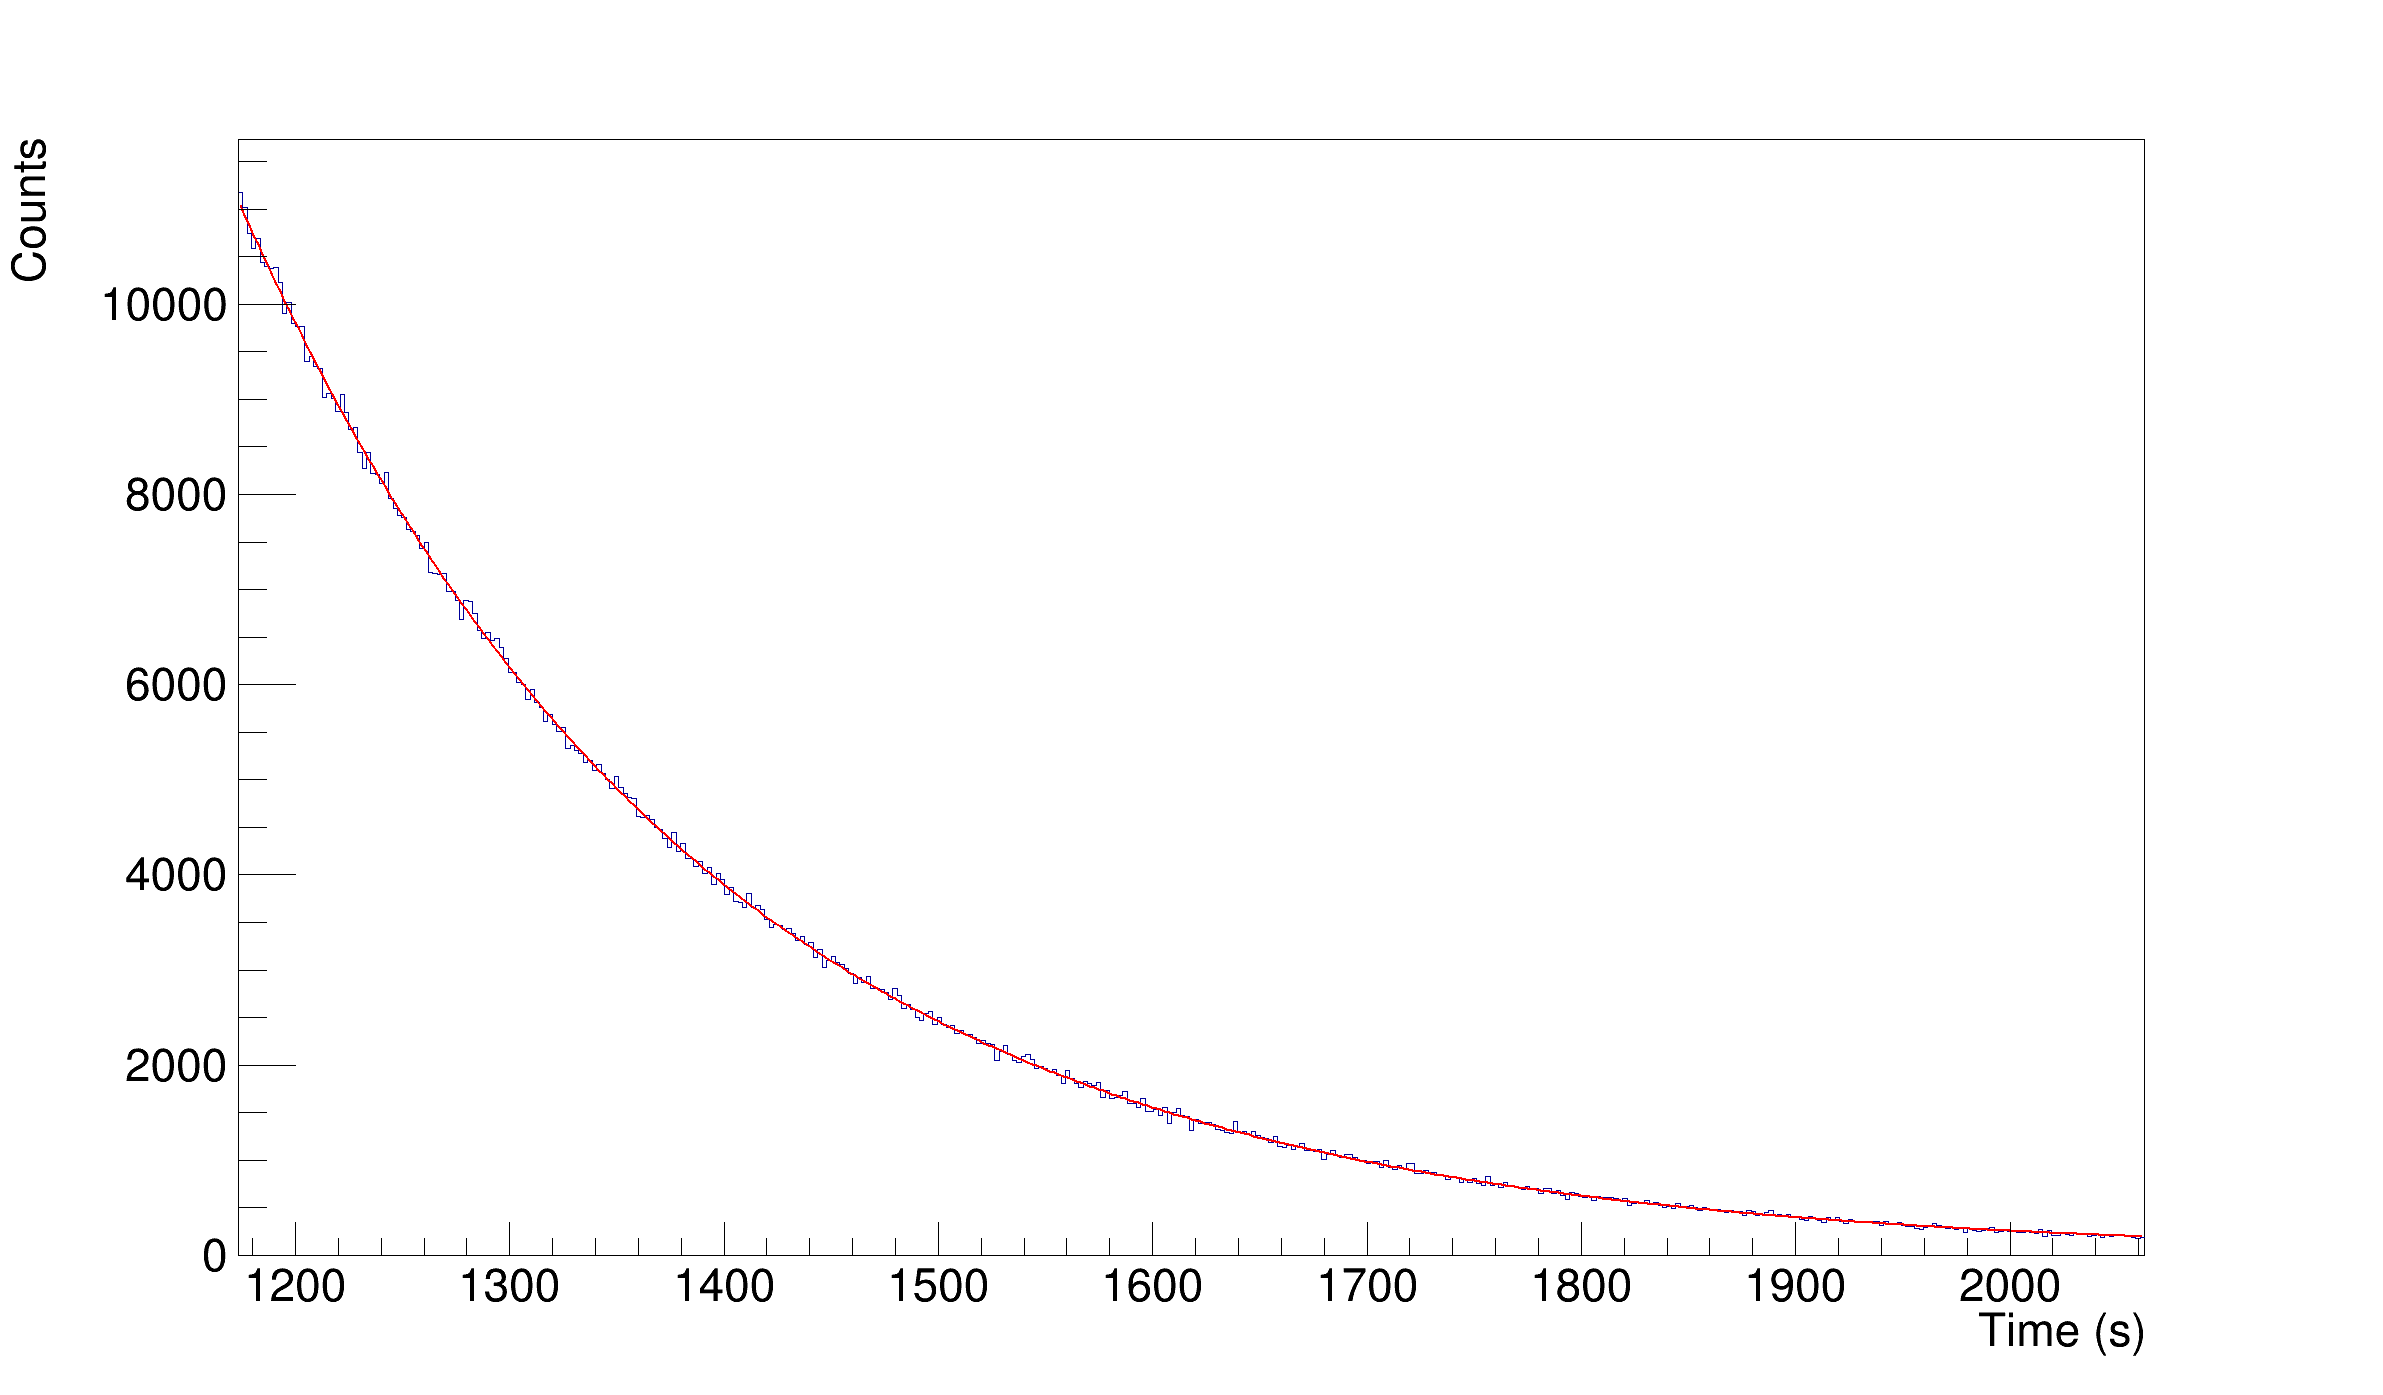
\includegraphics[width=\textwidth]{example_decay_fit.png}
	\caption{Example decay fit.}
	\label{example_decay_fit}
\end{figure}

We can solve the differential equation during the activation period analytically by taking $P(t)$ as a constant, $P$.
We get
\[ \ddt{N} = P -\lambda N  \]
and its solution is:
\begin{equation}
	N(t) = \frac{P}{\lambda} + \left(  N_0 - \frac{P}{\lambda}  \right) e^{-\lambda t}
\end{equation}
with $N_0$ the initial number of \Piso nuclei, assumed to be \num{0}.
$N$\textsubscript{EOA} will then be equal to:
\[ N\textsubscript{EOA} =N(\Delta t) = \frac{P}{\lambda} - \frac{P}{\lambda} e^{-\lambda \Delta t} = \frac{P}{\lambda} \left(1 - e^{-\lambda \Delta t} \right)\Longrightarrow A\textsubscript{EOA}=P\left(1-e^{-\lambda\Delta t}\right)\Longrightarrow \]
\begin{equation}
	P = \frac{A\textsubscript{EOA}}{1 - e^{-\lambda \Delta t}}
\end{equation}
with $\Delta t$ the total activation time.
As $P$ is the number of \Piso created per second, we can get the yield of the reaction by dividing over the number of incident alpha particles per unit of time:
\begin{equation}
	\text{yield} = \frac{P}{\text{alphas per second}} = \frac{A\textsubscript{EOA}}{\text{alphas per second} \cdot \left(1 - e^{-\lambda \Delta t} \right)}
\end{equation}

All that is left is to correct for the efficiency of the detector, and the final formula for the thick target yield is:
\begin{equation}
	\text{yield} = \frac{A\textsubscript{EOA}}{\text{alphas per second} \cdot \text{detector efficiency} \cdot \left(1 - e^{-\lambda \Delta t} \right) \cdot 1.99}	%TBD? use symbols instead?
\end{equation}

\subsubsection{Unified and rise fit}
Instead of taking $P(t)$ as a constant, we can fit either the whole histogram or the activation period (\textit{unified} and \textit{rise} fits, respectively) to a function that integrates equation \ref{activation_diffeq} by taking $P(t)$ as proportional to the current step by step.
This is useful because the current is not constant, there are drops and rises in many of the measurements (figure \ref{current_histograms}) and this will make the \textit{decay} fit less precise, as the assumption of constant current is incorrect.

\begin{figure}[H]
	\centering
	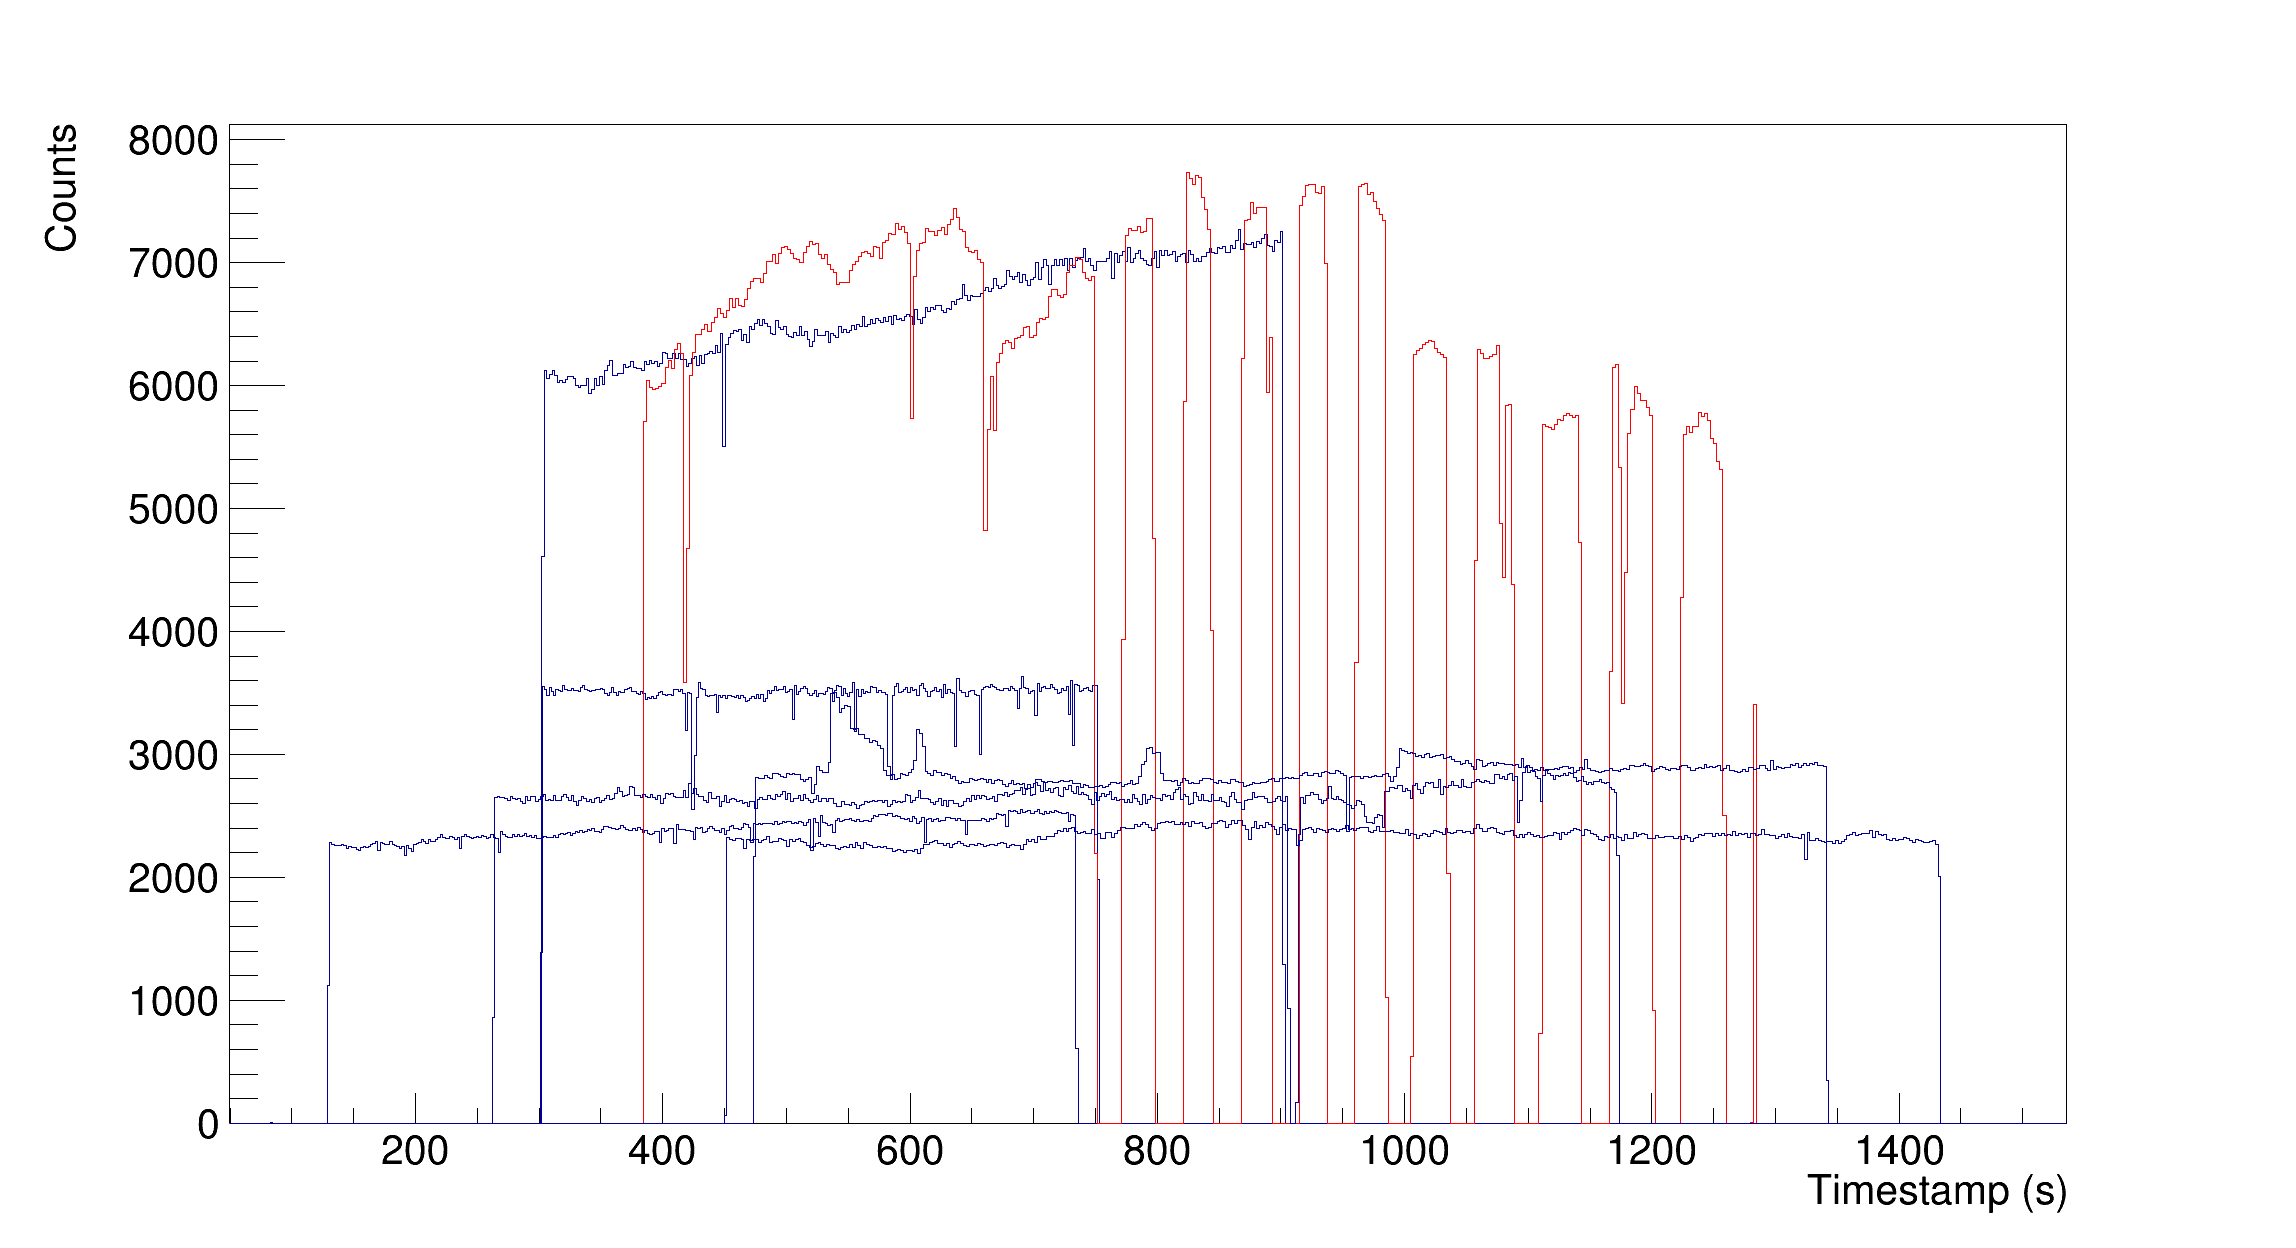
\includegraphics[width=\textwidth]{current_histograms.png}
	\caption{All current histograms, superimposed.
	The one in red corresponds to measurement 4.}
	\label{current_histograms}
\end{figure}

This function also considers a constant background, an initial number of \Piso (from previous activation runs); and a number of counts proportional to the current, which correspond to gamma rays being produced by reactions other than \an.	%TBD:like?

The fit returns the \an yield directly, but in units of number of reactions per \qty{0.1}{\nano\coulomb} per binwidth.
Thus the yield, corrected by the detector efficiency, in \an per alpha, is:
\begin{equation}
	\text{yield} = \frac{\text{fit result}}{2\cdot1.60217646\cdot10^{-9}\cdot 1.99 \cdot \text{detector efficiency}}
\end{equation}
with $2\cdot\num{1.60217646E-9}$ the charge of an alpha particle in tenths of nanocoulombs.
\\

\begin{figure}[H]
	\centering
	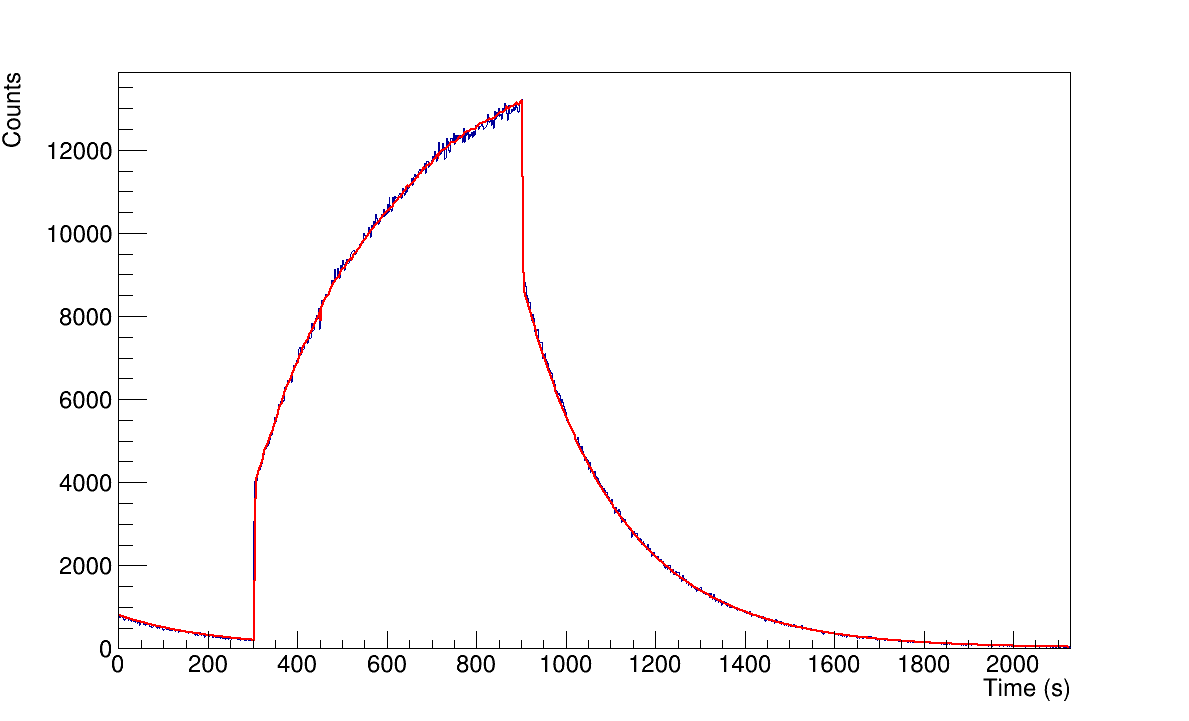
\includegraphics[width=\textwidth]{example_unified_fit.png}
	\caption{Example unified fit.}
	\label{example_unified_fit}
\end{figure}

\begin{figure}[H]
	\centering
	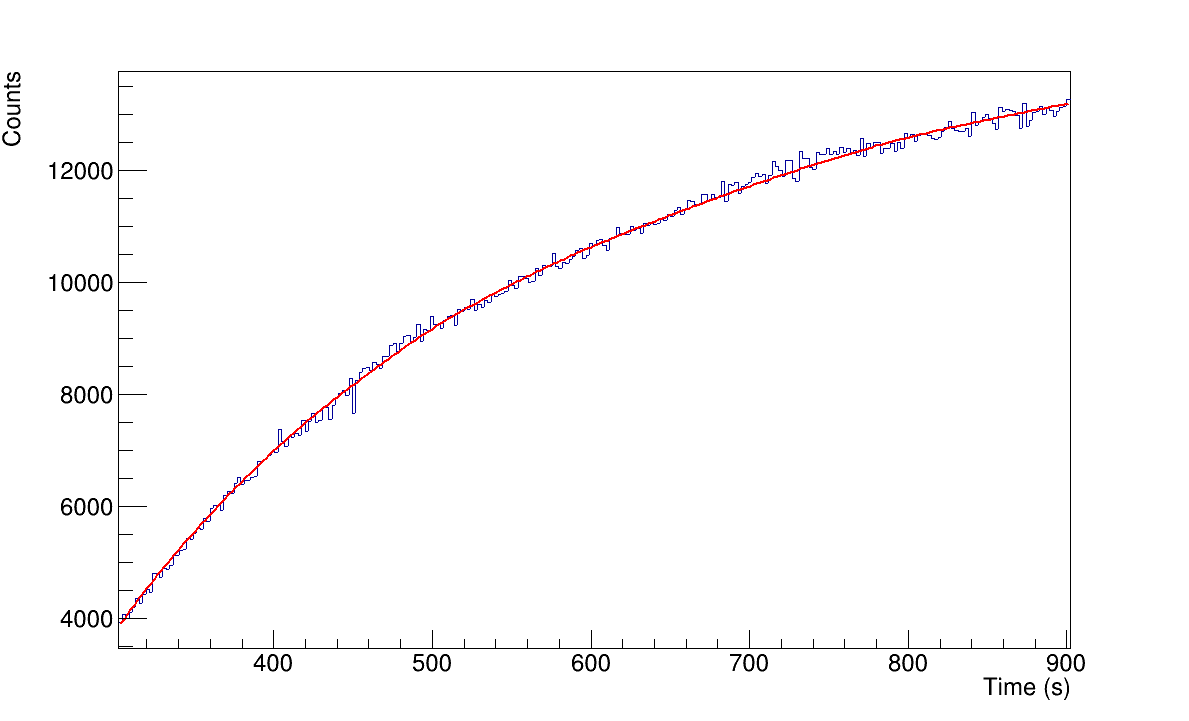
\includegraphics[width=\textwidth]{example_rise_fit.png}
	\caption{Example rise fit.}
	\label{example_rise_fit}
\end{figure}

Data of current over time was not recorded in half of the measurements in April (numbers 8, 9 and 10).	%TBD: por qué razón?
In addition, measurement number 4, in February, shows loss of data due to a problem with the DAQ.

\begin{figure}[H]
	\centering
	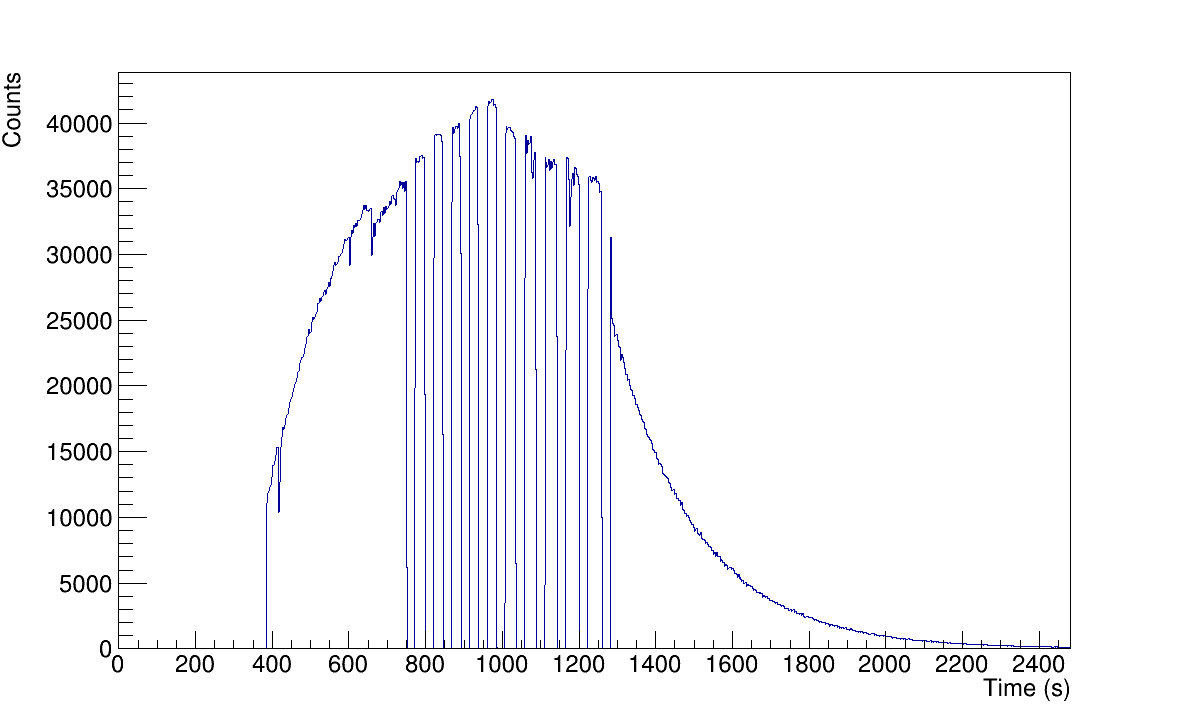
\includegraphics[width=\textwidth]{activation_4_time.png}
	\caption{Activation measurement number 4.}
	\label{activation_4_time}
\end{figure}

These problems prevent the \textit{unified} and \textit{rise} fits to be used for all measurements.
\\

\subsection{Results}
Figure \ref{decay_errors_rel_per} shows that the relative difference in measurements between LaBr detectors 1 and 2 is under \qty{10}{\percent}.
The numbers are for decay fit measurements, but are similar for the other methods.
Measurements in February show negative values, indicating detector 2 is higher; while those in April are positive, meaning the opposite is true.

\begin{figure}[H]
	\centering
	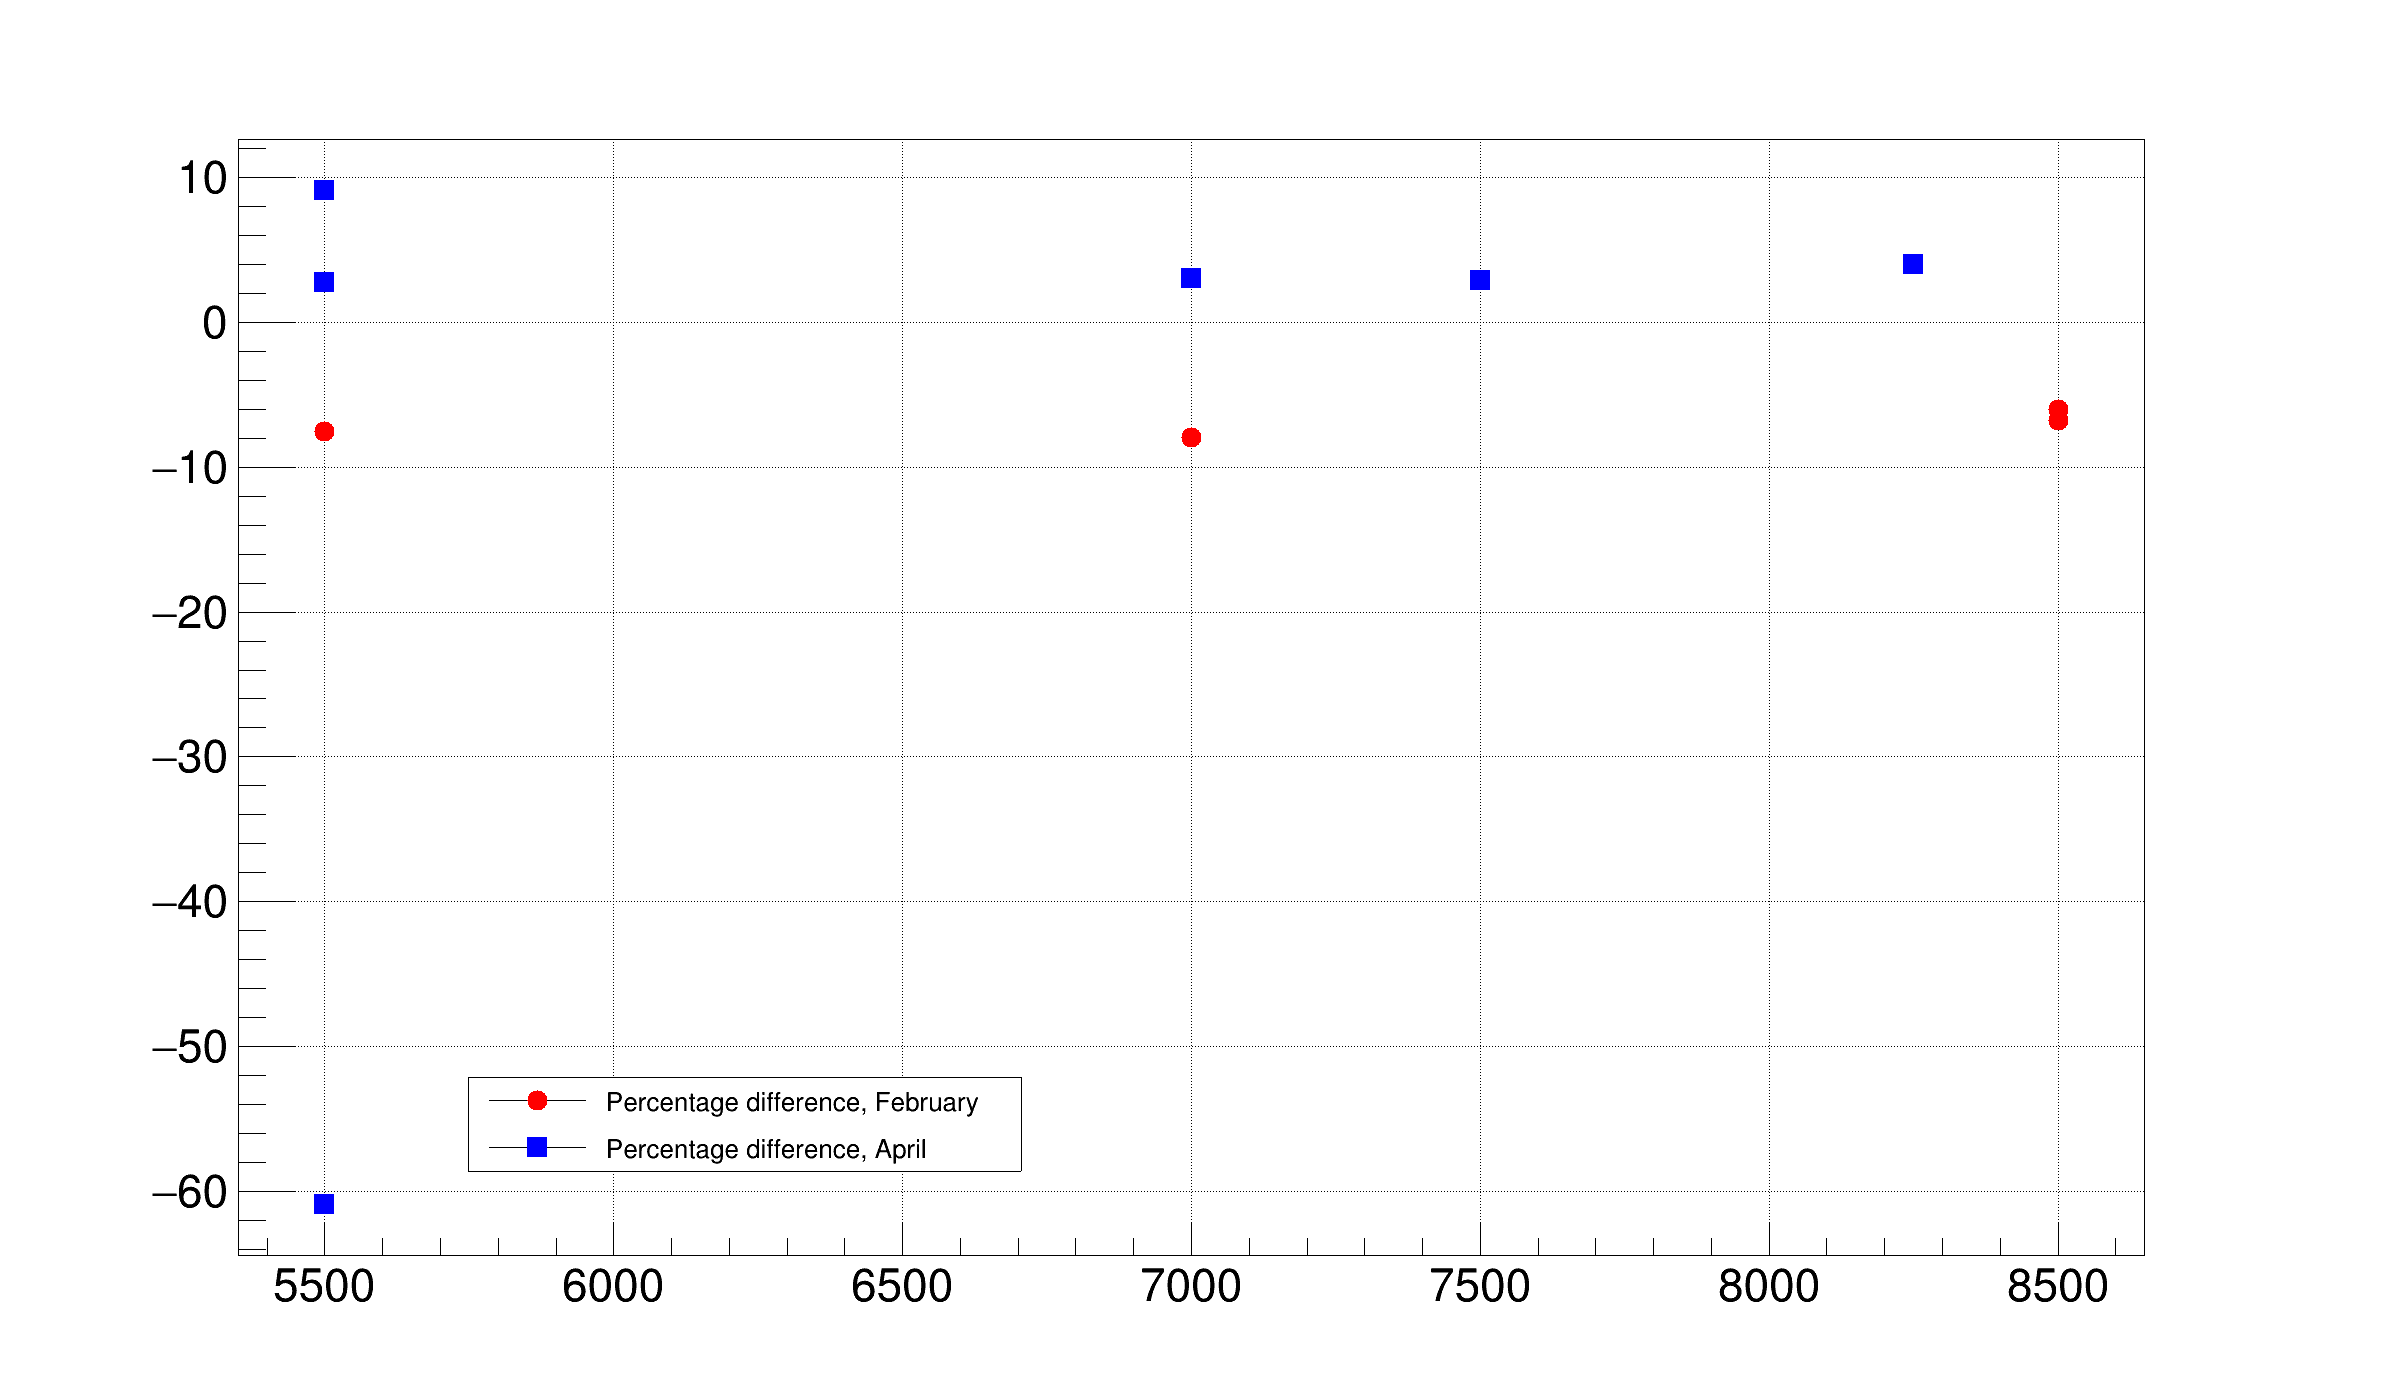
\includegraphics[width=\textwidth]{decay_errors_rel_per.png}
	\caption{Percentage difference in thick target yield results between detectors in each measurement.
	The number shown is calculated as $\frac{\text{det}1-\text{det}2}{\left(\text{det}1+\text{det}2\right)/2}\cdot 100$, the difference over the average, in percentage.}
	\label{decay_errors_rel_per}
\end{figure}

The outlier, with \qty{-60}{\percent}, corresponds to measurement number 6.
For this measurement, LaBr detector number 1 was placed much closer to the target, and at \qty{0}{\degree}.
The corresponding \Na calibration measurement may not correspond to that exact configuration, and so the results from this measurement and detector are probably unreliable.
The measurements \emph{before} the change in position can also not be trusted, as the calibration was done on the 18th, after the position change.
\\

The best agreements between detectors are for the measurements in April 18th, under \qty{5}{\percent}.
In figure \ref{decay_errors_per}, we can see that decay fit results are between \qty{10}{\percent} and \qty{5}{\percent} smaller than EXFOR data for the measurements in April 18th, but more than \qty{50}{\percent} smaller for February.
The April 17th results are around \qty{30}{\percent}, and the \textit{outlier} from before is at \qty{60}{\percent}.

\begin{figure}[H]
	\centering
	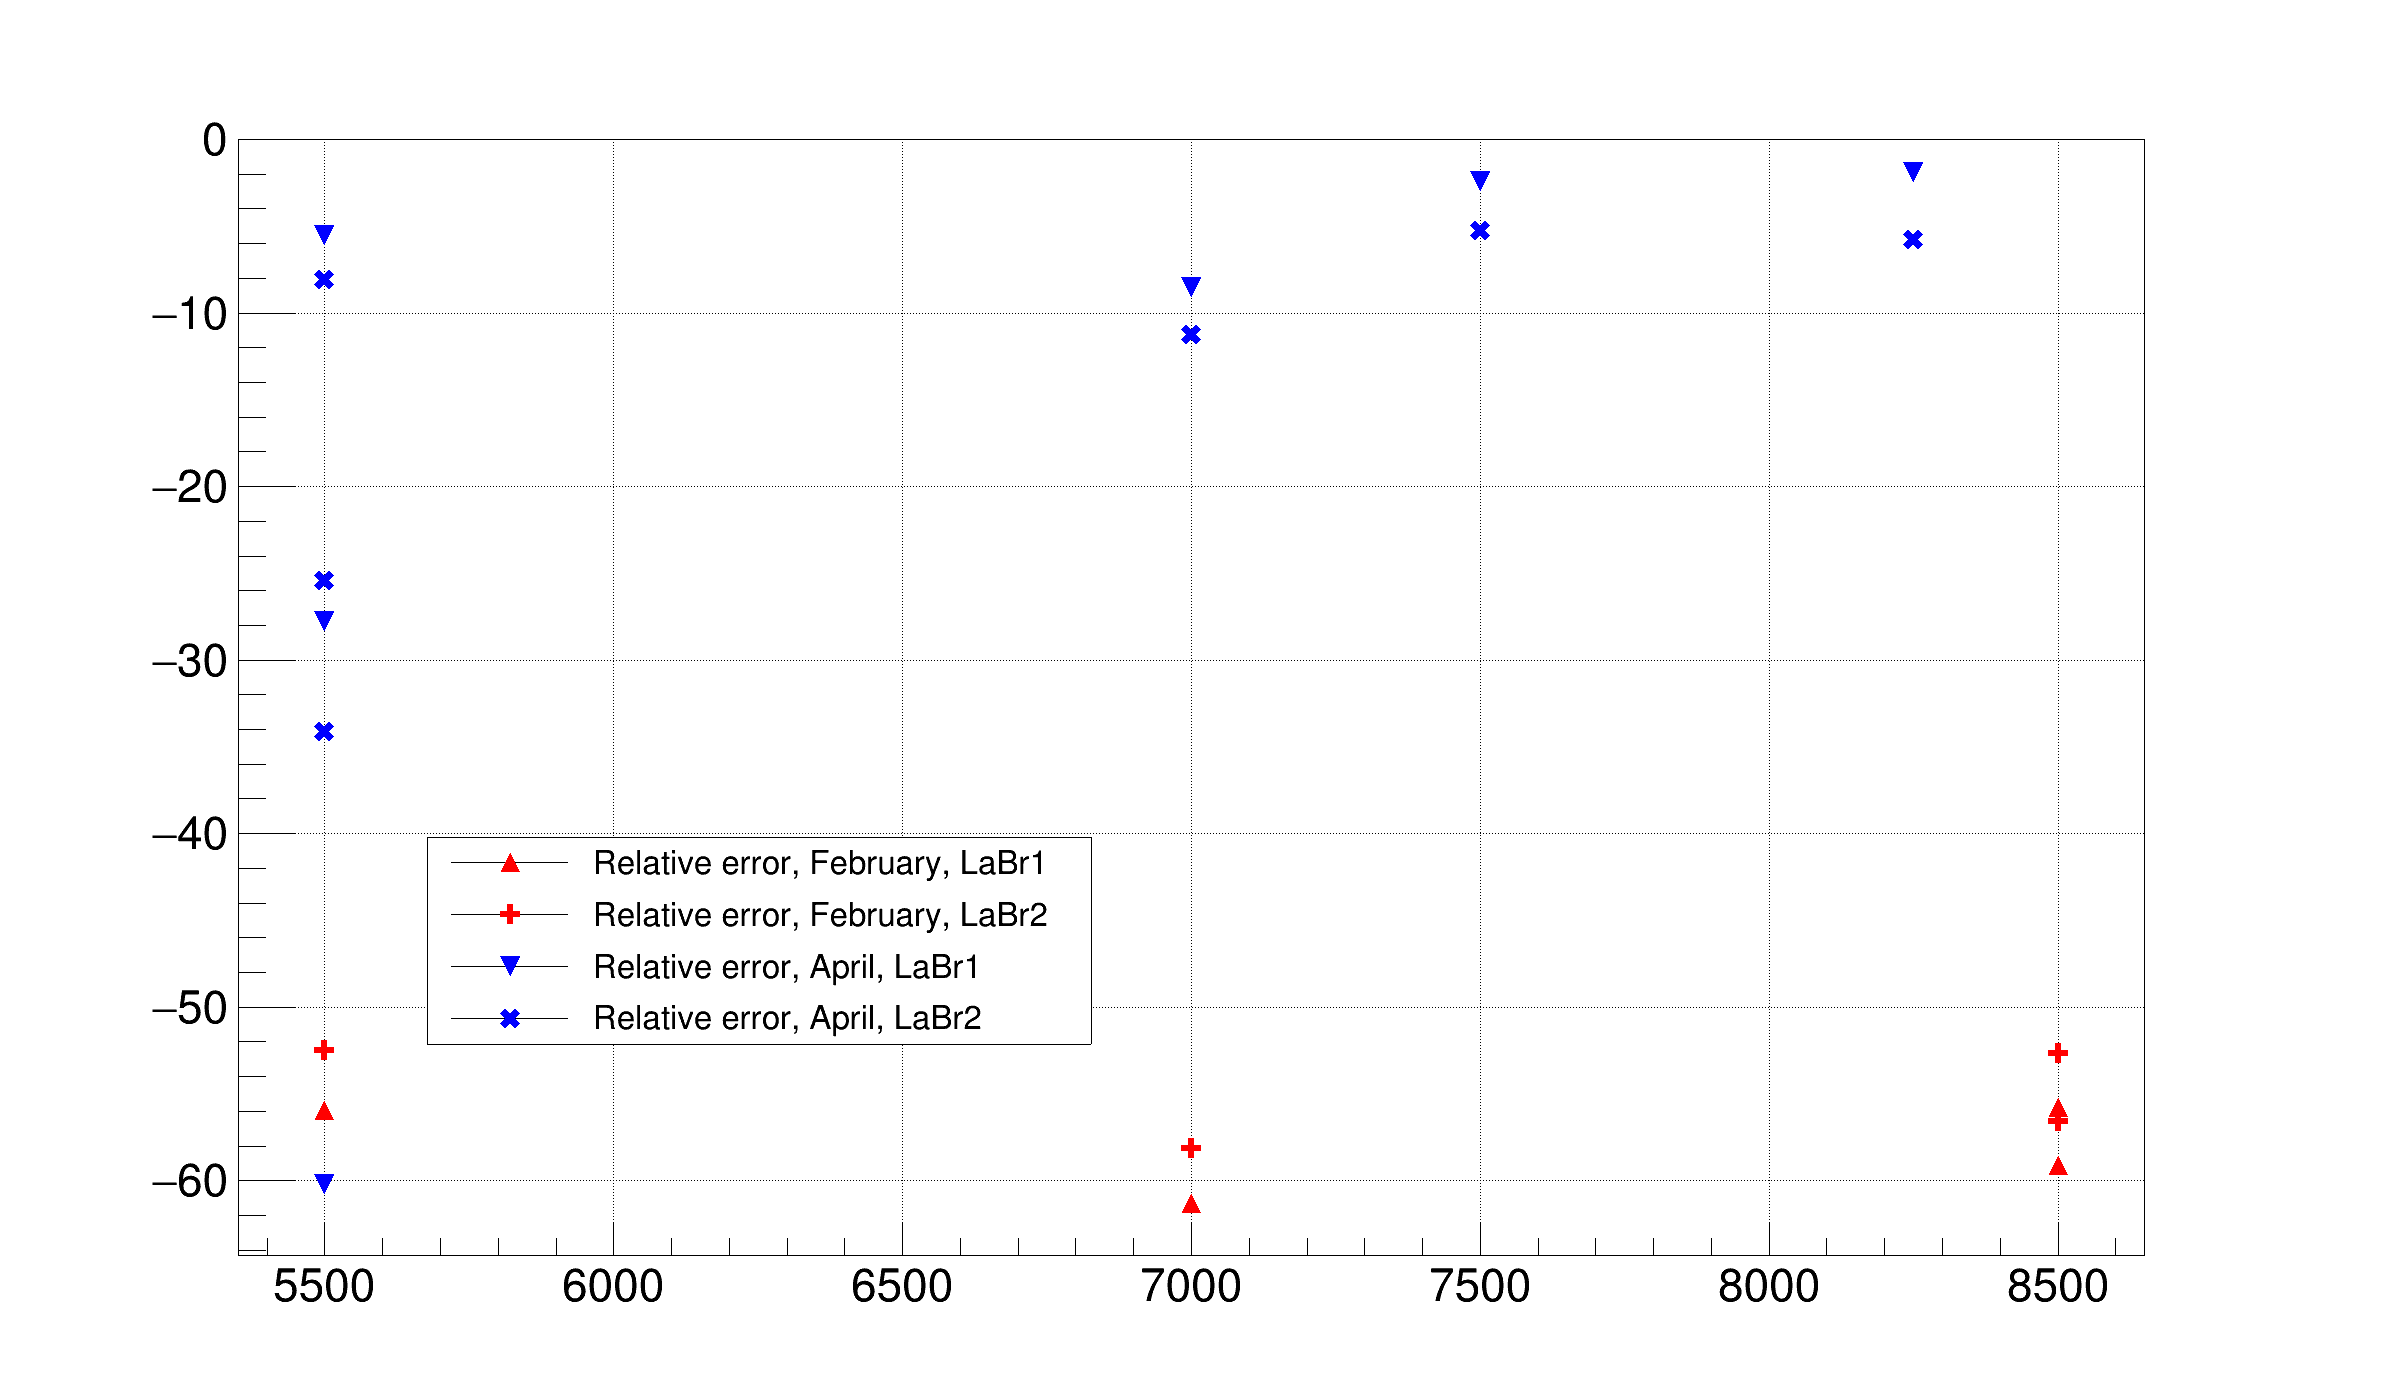
\includegraphics[width=\textwidth]{decay_errors_per.png}
	\caption{Percentage difference in thick target yield results between each \textit{decay} fit measurement and EXFOR.}
	\label{decay_errors_per}
\end{figure}

In short, \textit{decay} fit thick target yield results agree relatively well with EXFOR data only for the measurements done in April 18th.
The ones done in April 17th are suspect, and the ones in February agree with each other (have the same shape as the EXFOR data) but are off by a factor of $\approx 2$.

\begin{figure}[H]
	\centering
	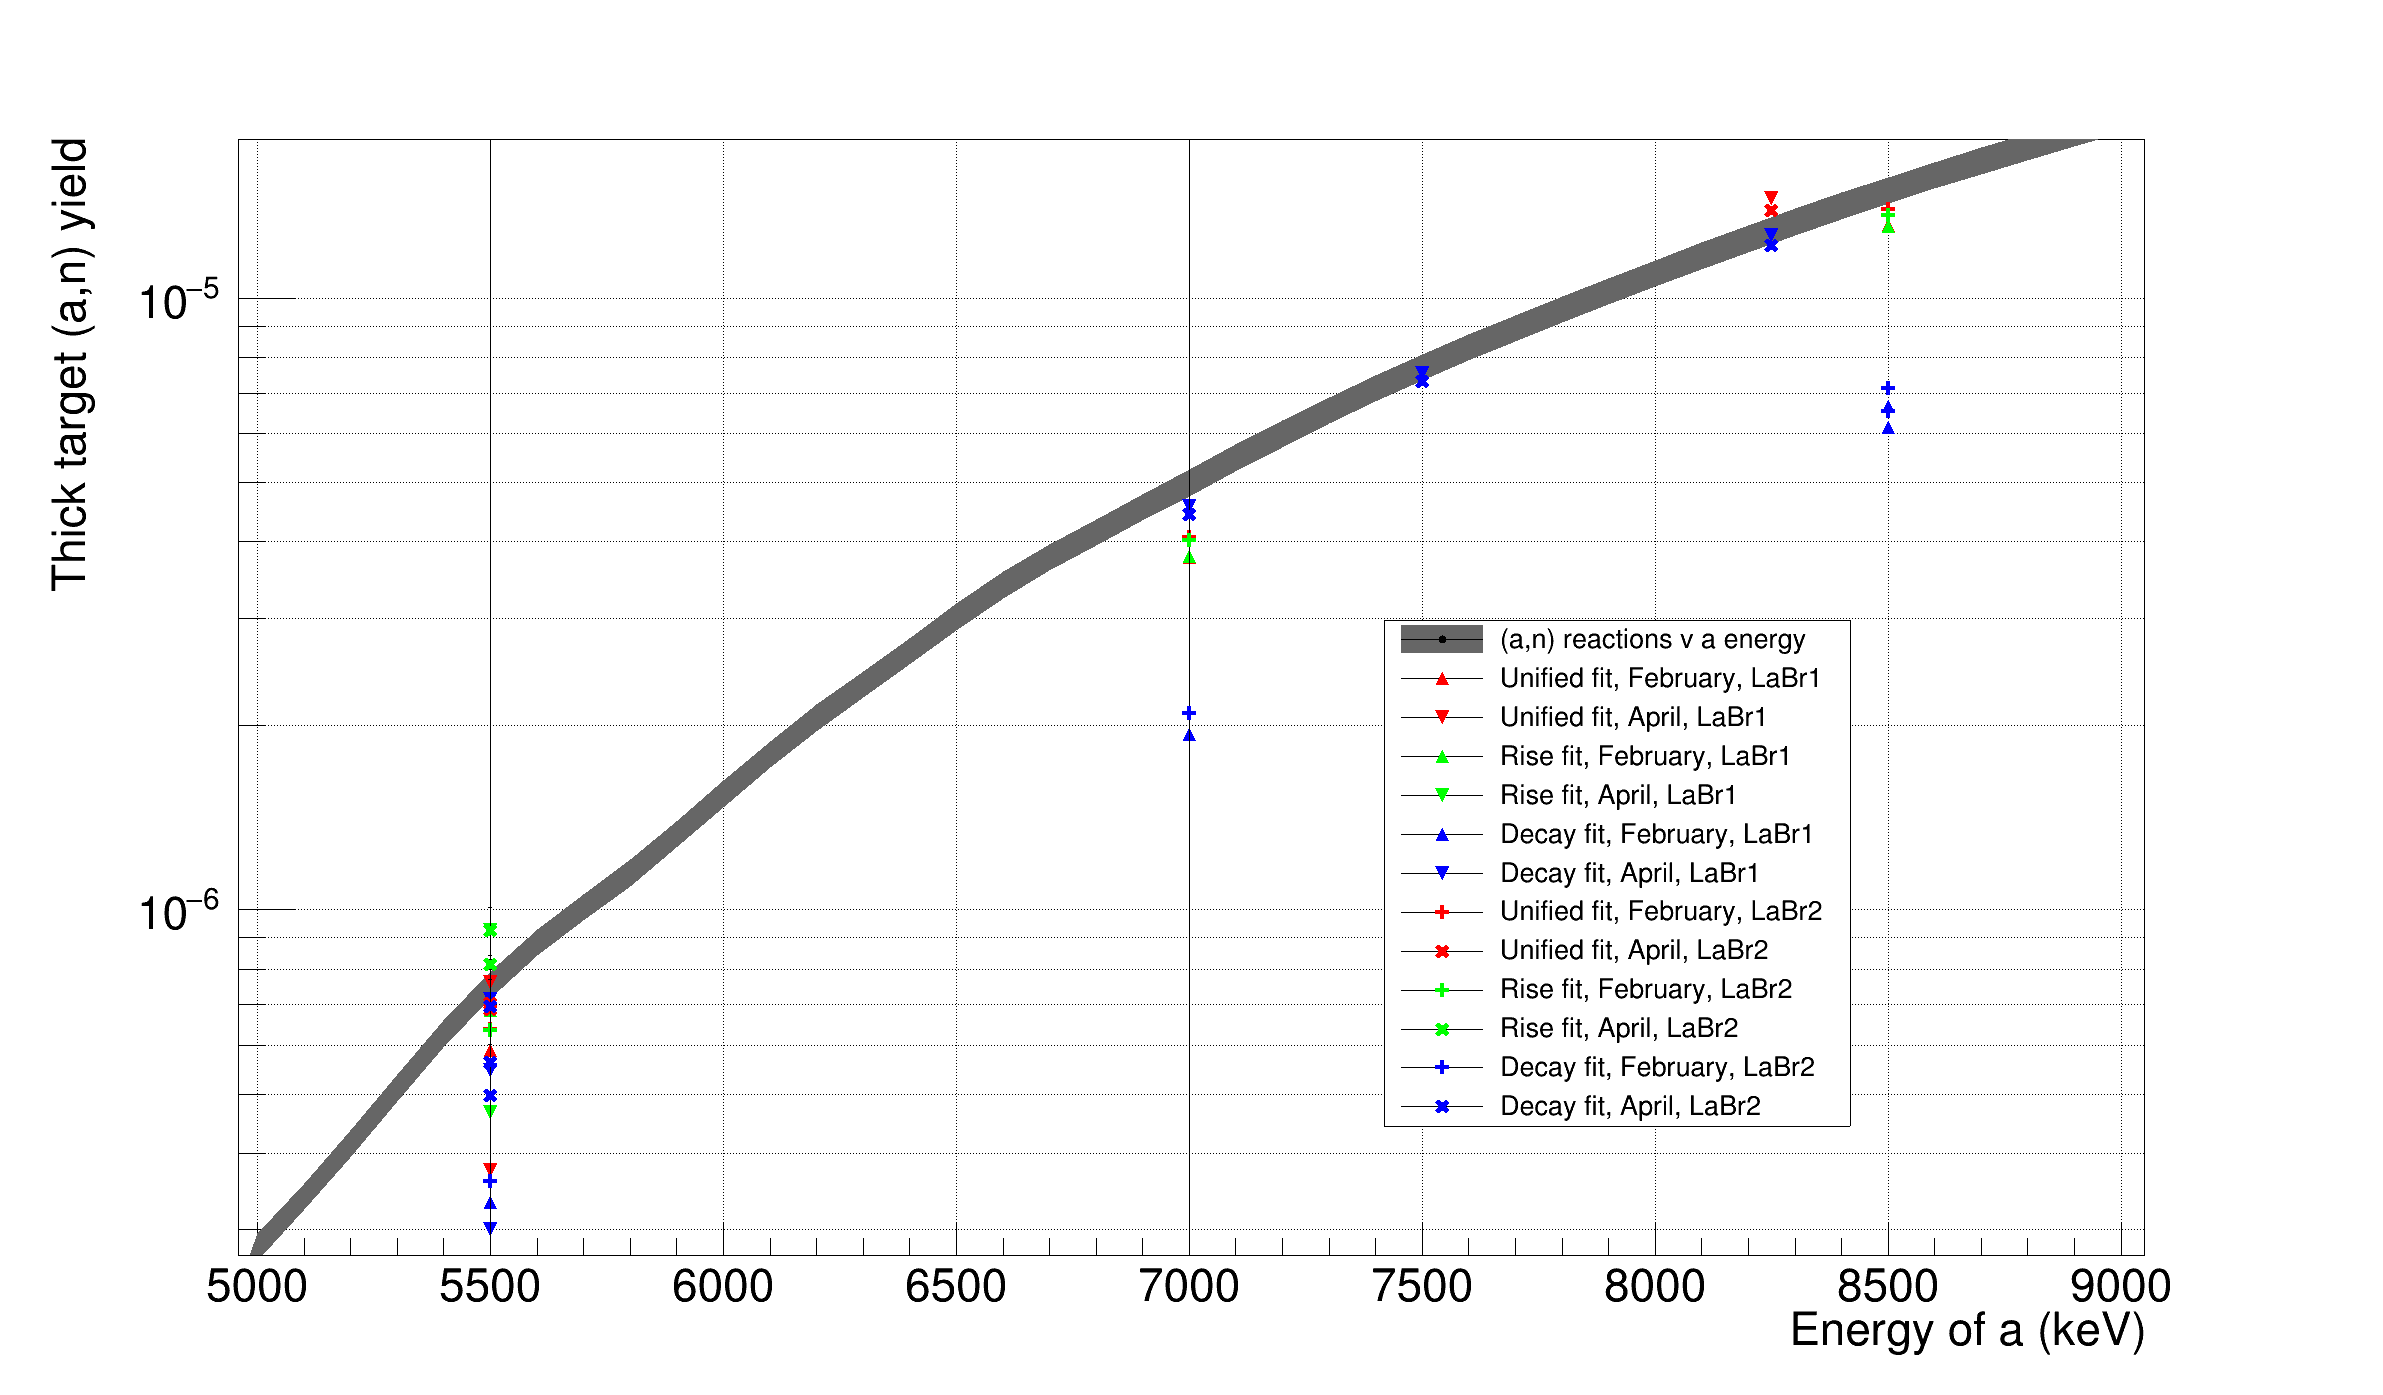
\includegraphics[width=\textwidth]{reactions_v_energy_decay.png}
	\caption{Decay fit results and EXFOR data with a \qty{\pm 10}{\percent} error.}
	\label{reactions_v_energy_decay}
\end{figure}

We can compare this with the results obtained with \textit{rise} and \textit{unified} fits, in figures \ref{rise_errors_per} and \ref{unified_errors_per}.
Both also show February results as smaller than April, but the difference is much smaller.
Because of the missing current data, however, fewer points exist for April.

\begin{figure}[H]
	\centering
	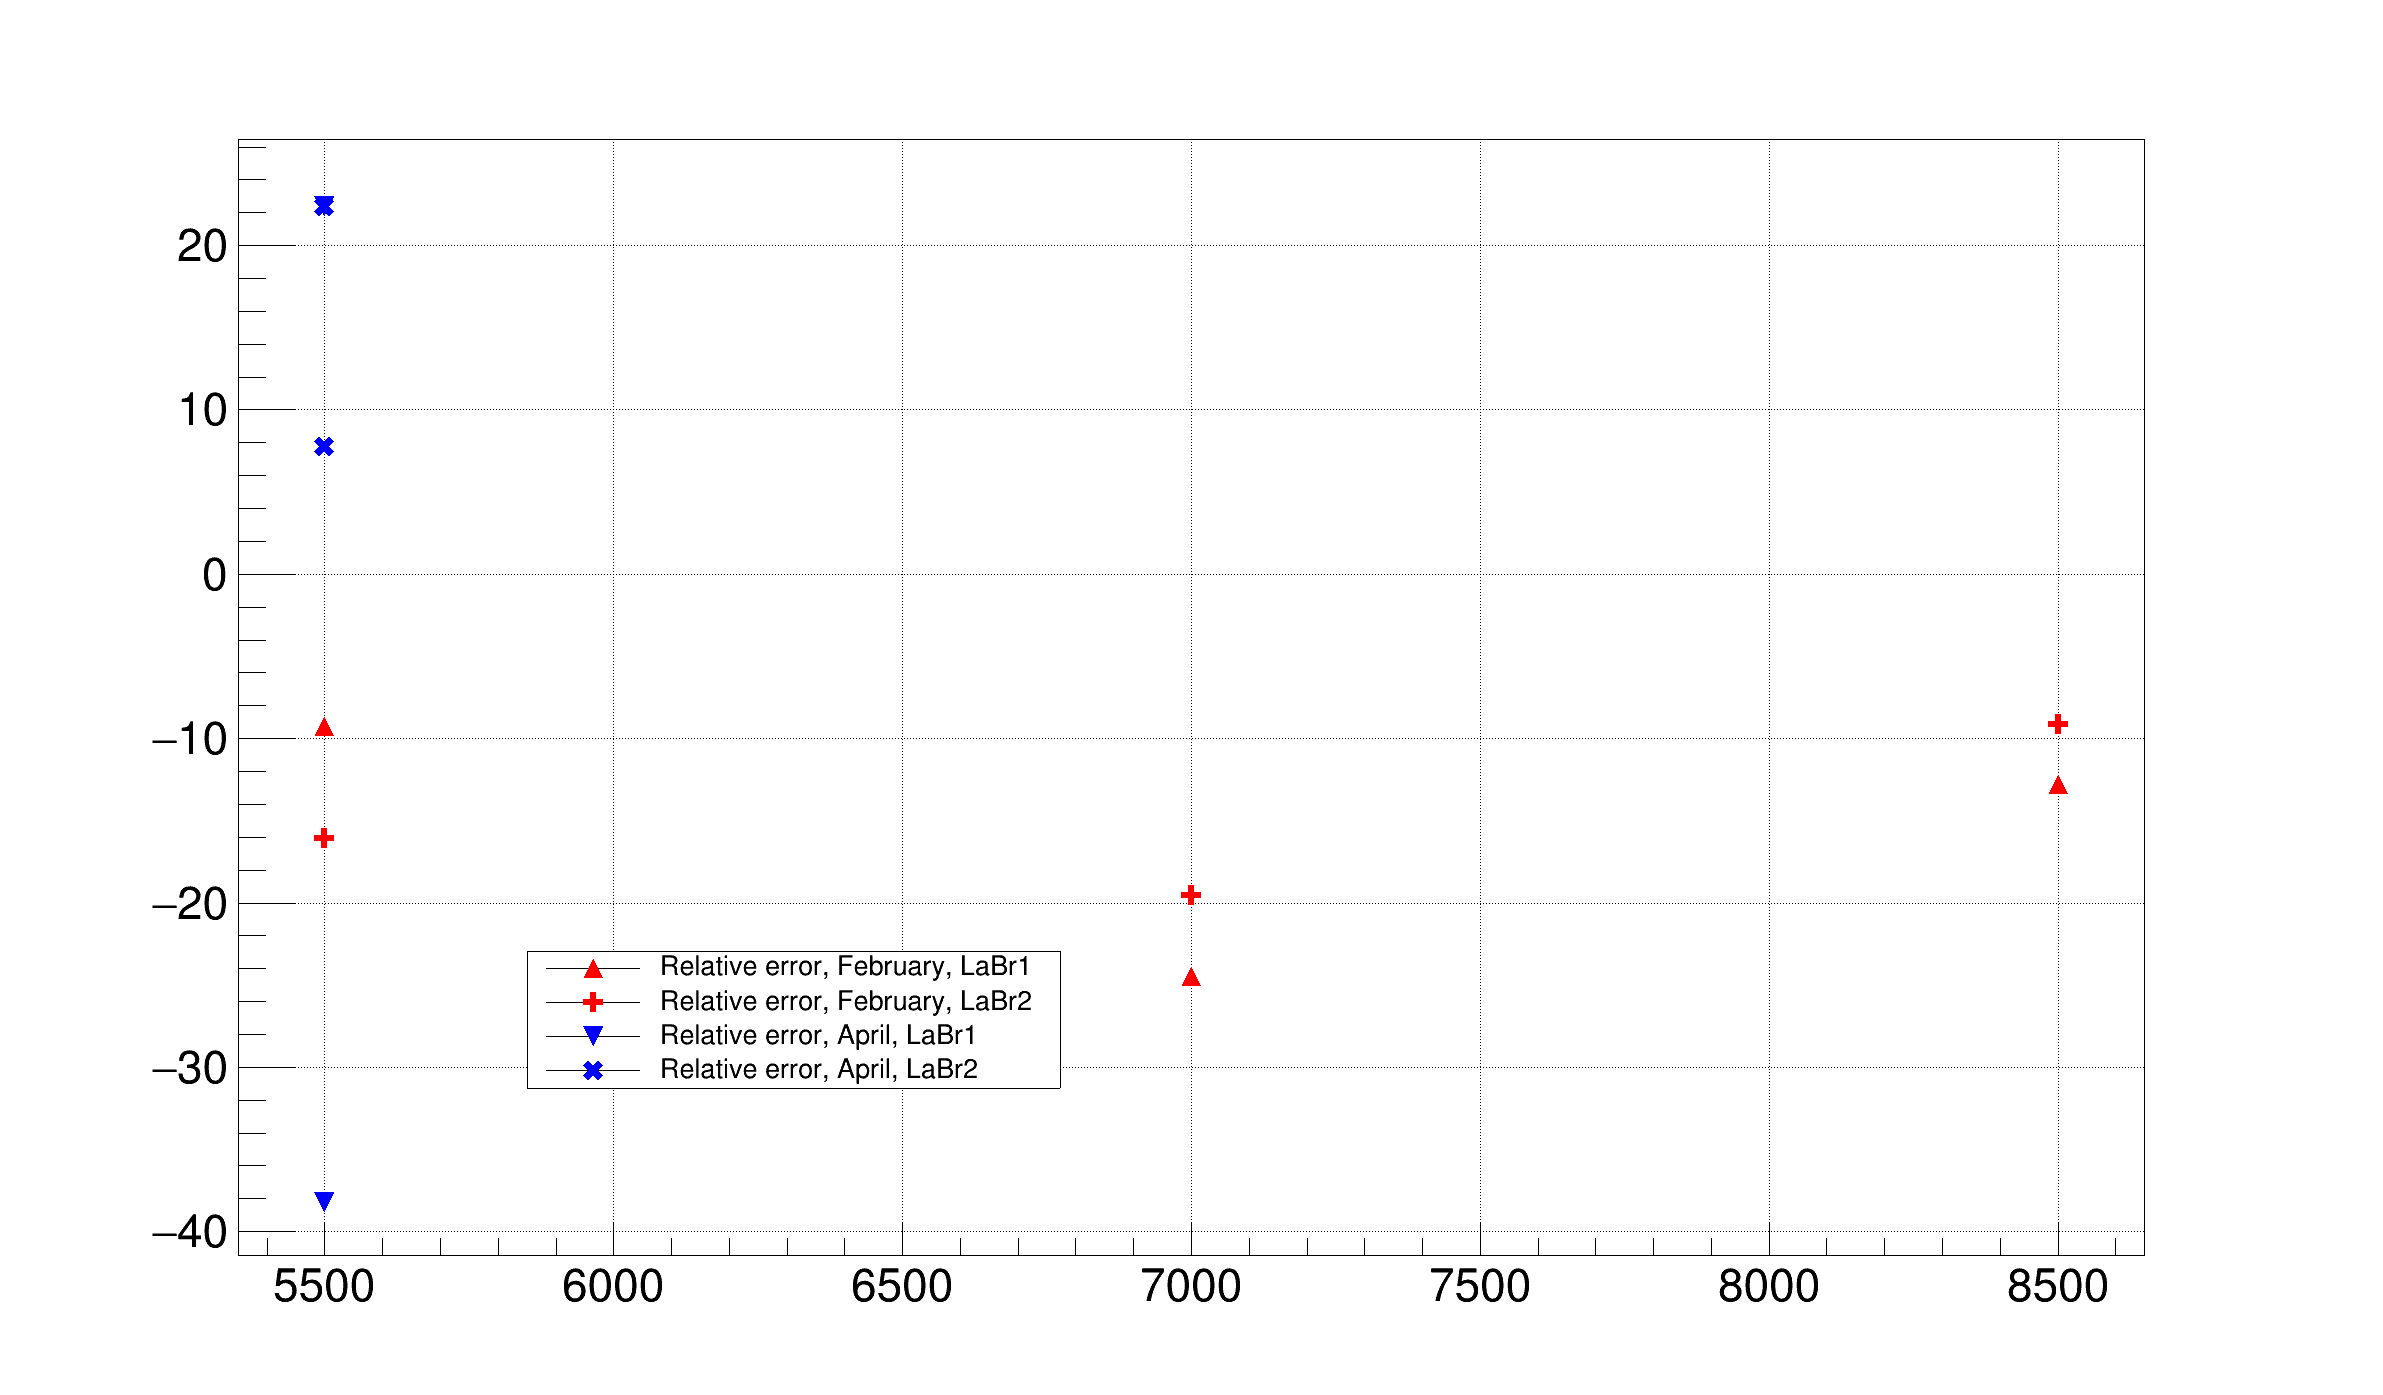
\includegraphics[width=\textwidth]{rise_errors_per.png}
	\caption{Percentage difference in thick target yield results between each \textit{rise} fit measurement and EXFOR.}
	\label{rise_errors_per}
\end{figure}

For the \textit{rise} fits, there are no points for April 18th, as the only measurement on the 18th with current data has a few extra counts outside the activation period, throwing off the algorithm that determines the exact start and end of the activation period.
Both February and April show, however, similar differences with respect to EXFOR data: around \qty{-15}{\percent} for February and around \qty{+20}{\percent} for April 17th.

\begin{figure}[H]
	\centering
	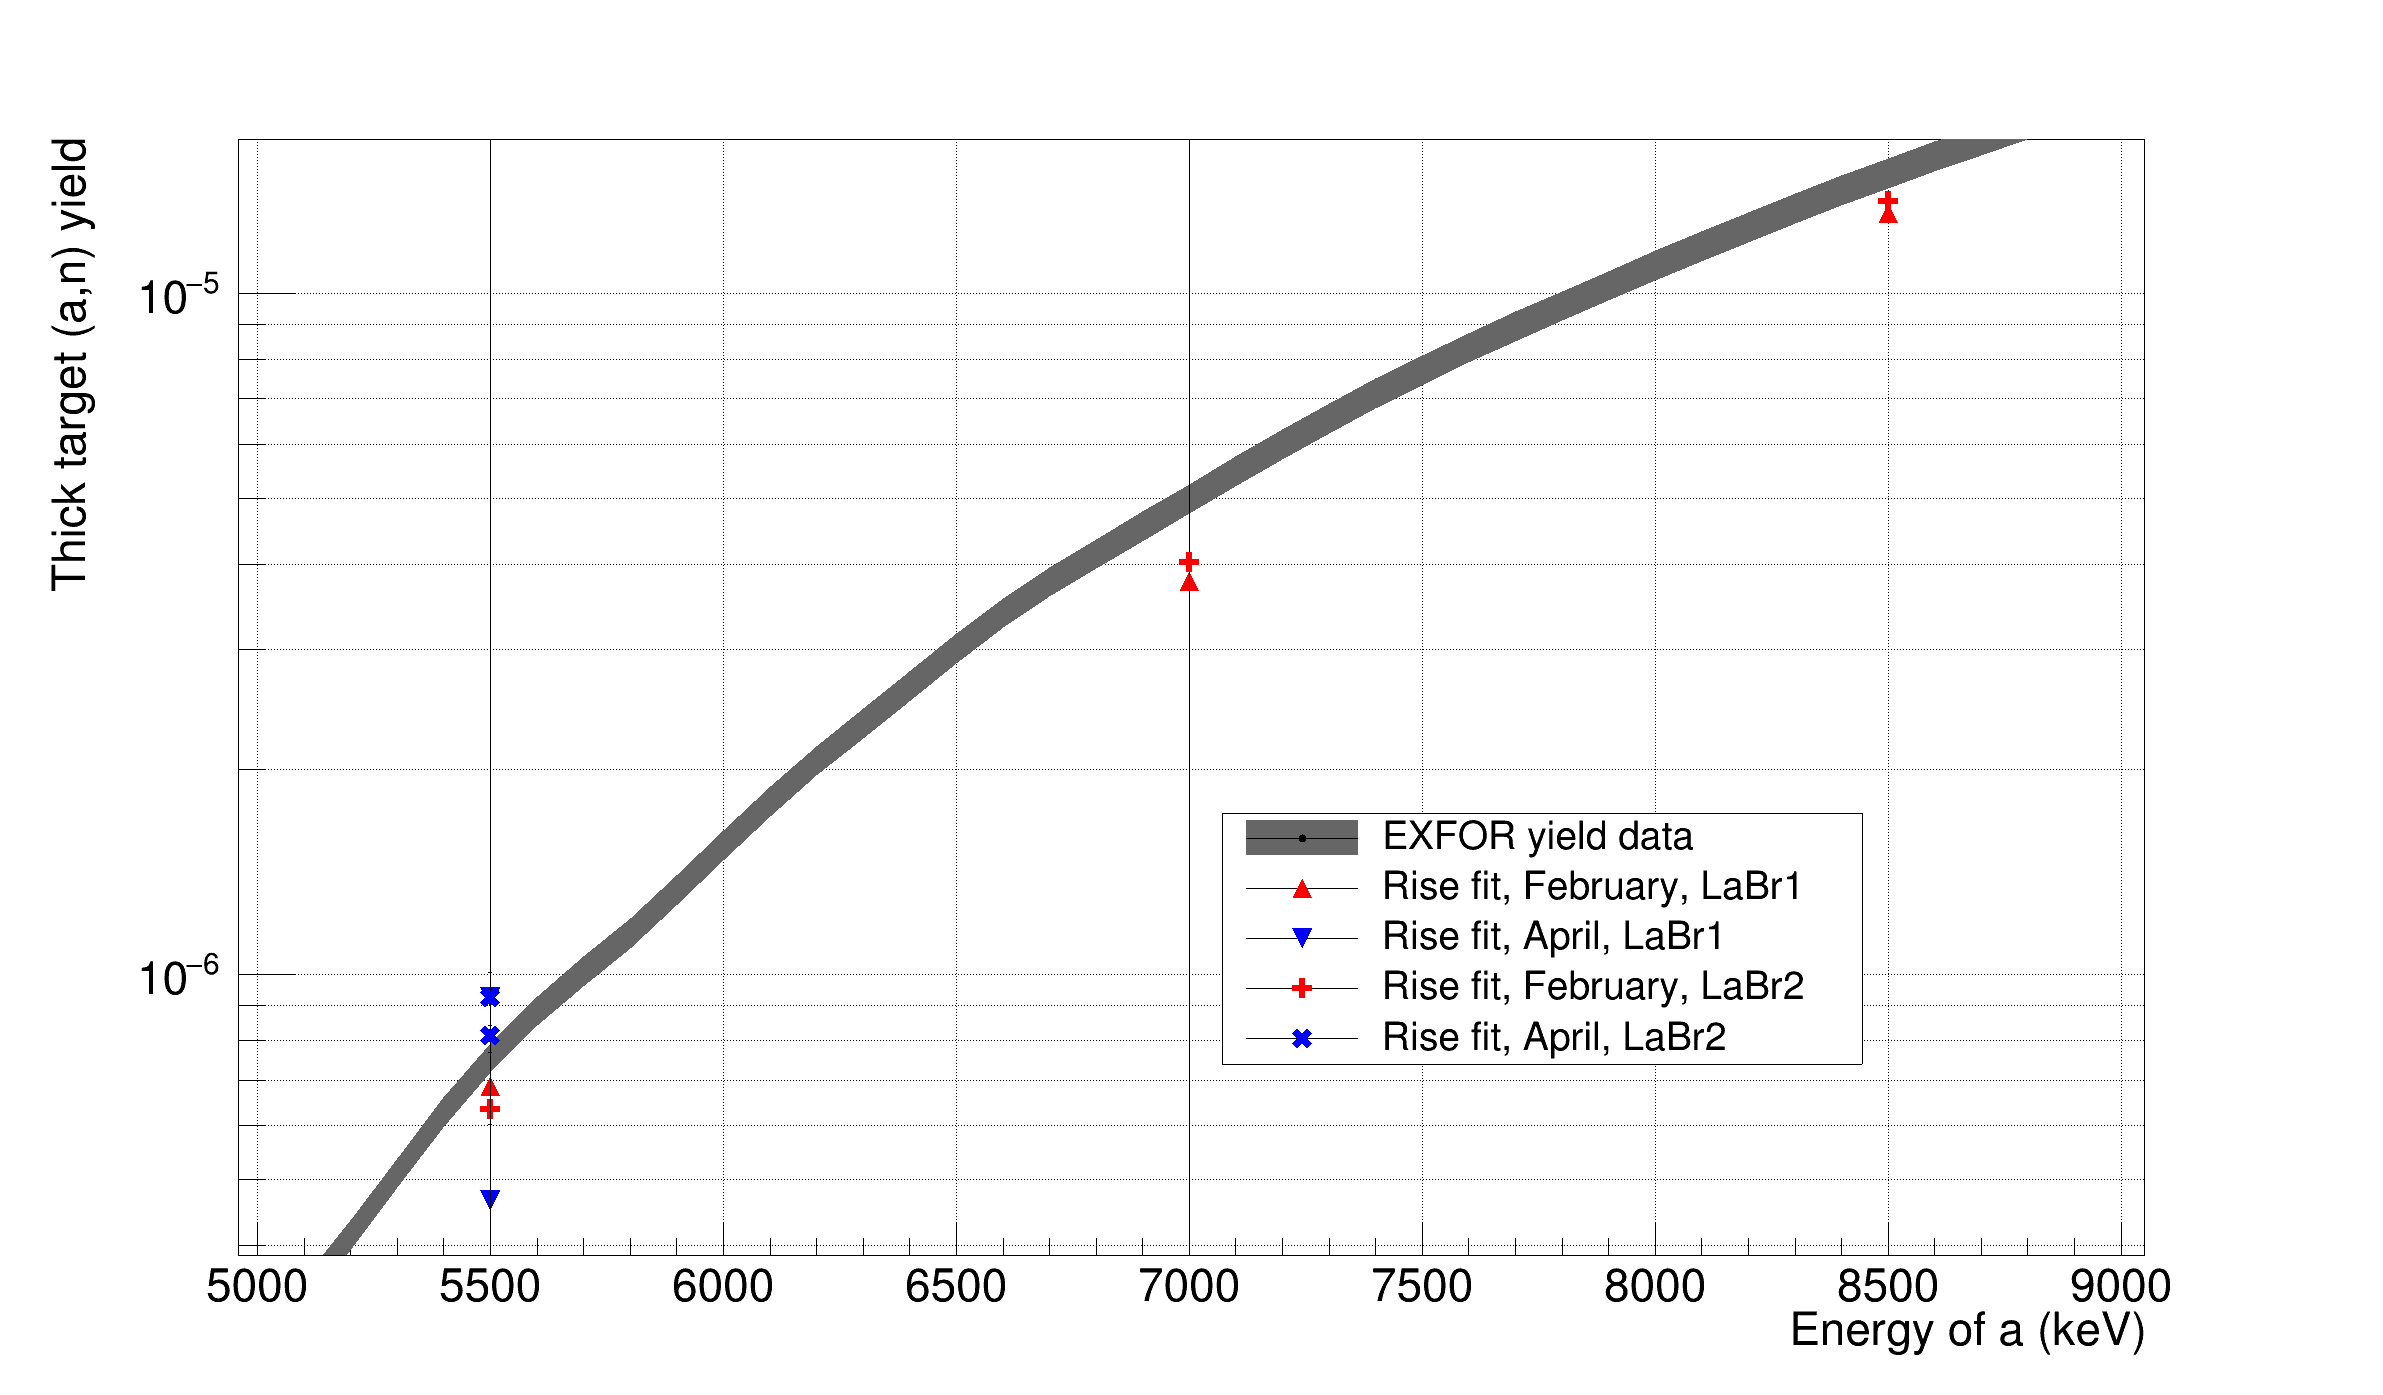
\includegraphics[width=\textwidth]{reactions_v_energy_rise.png}
	\caption{Rise fit results and EXFOR data with a \qty{\pm 10}{\percent} error.}
	\label{reactions_v_energy_rise}
\end{figure}

\begin{figure}[H]
	\centering
	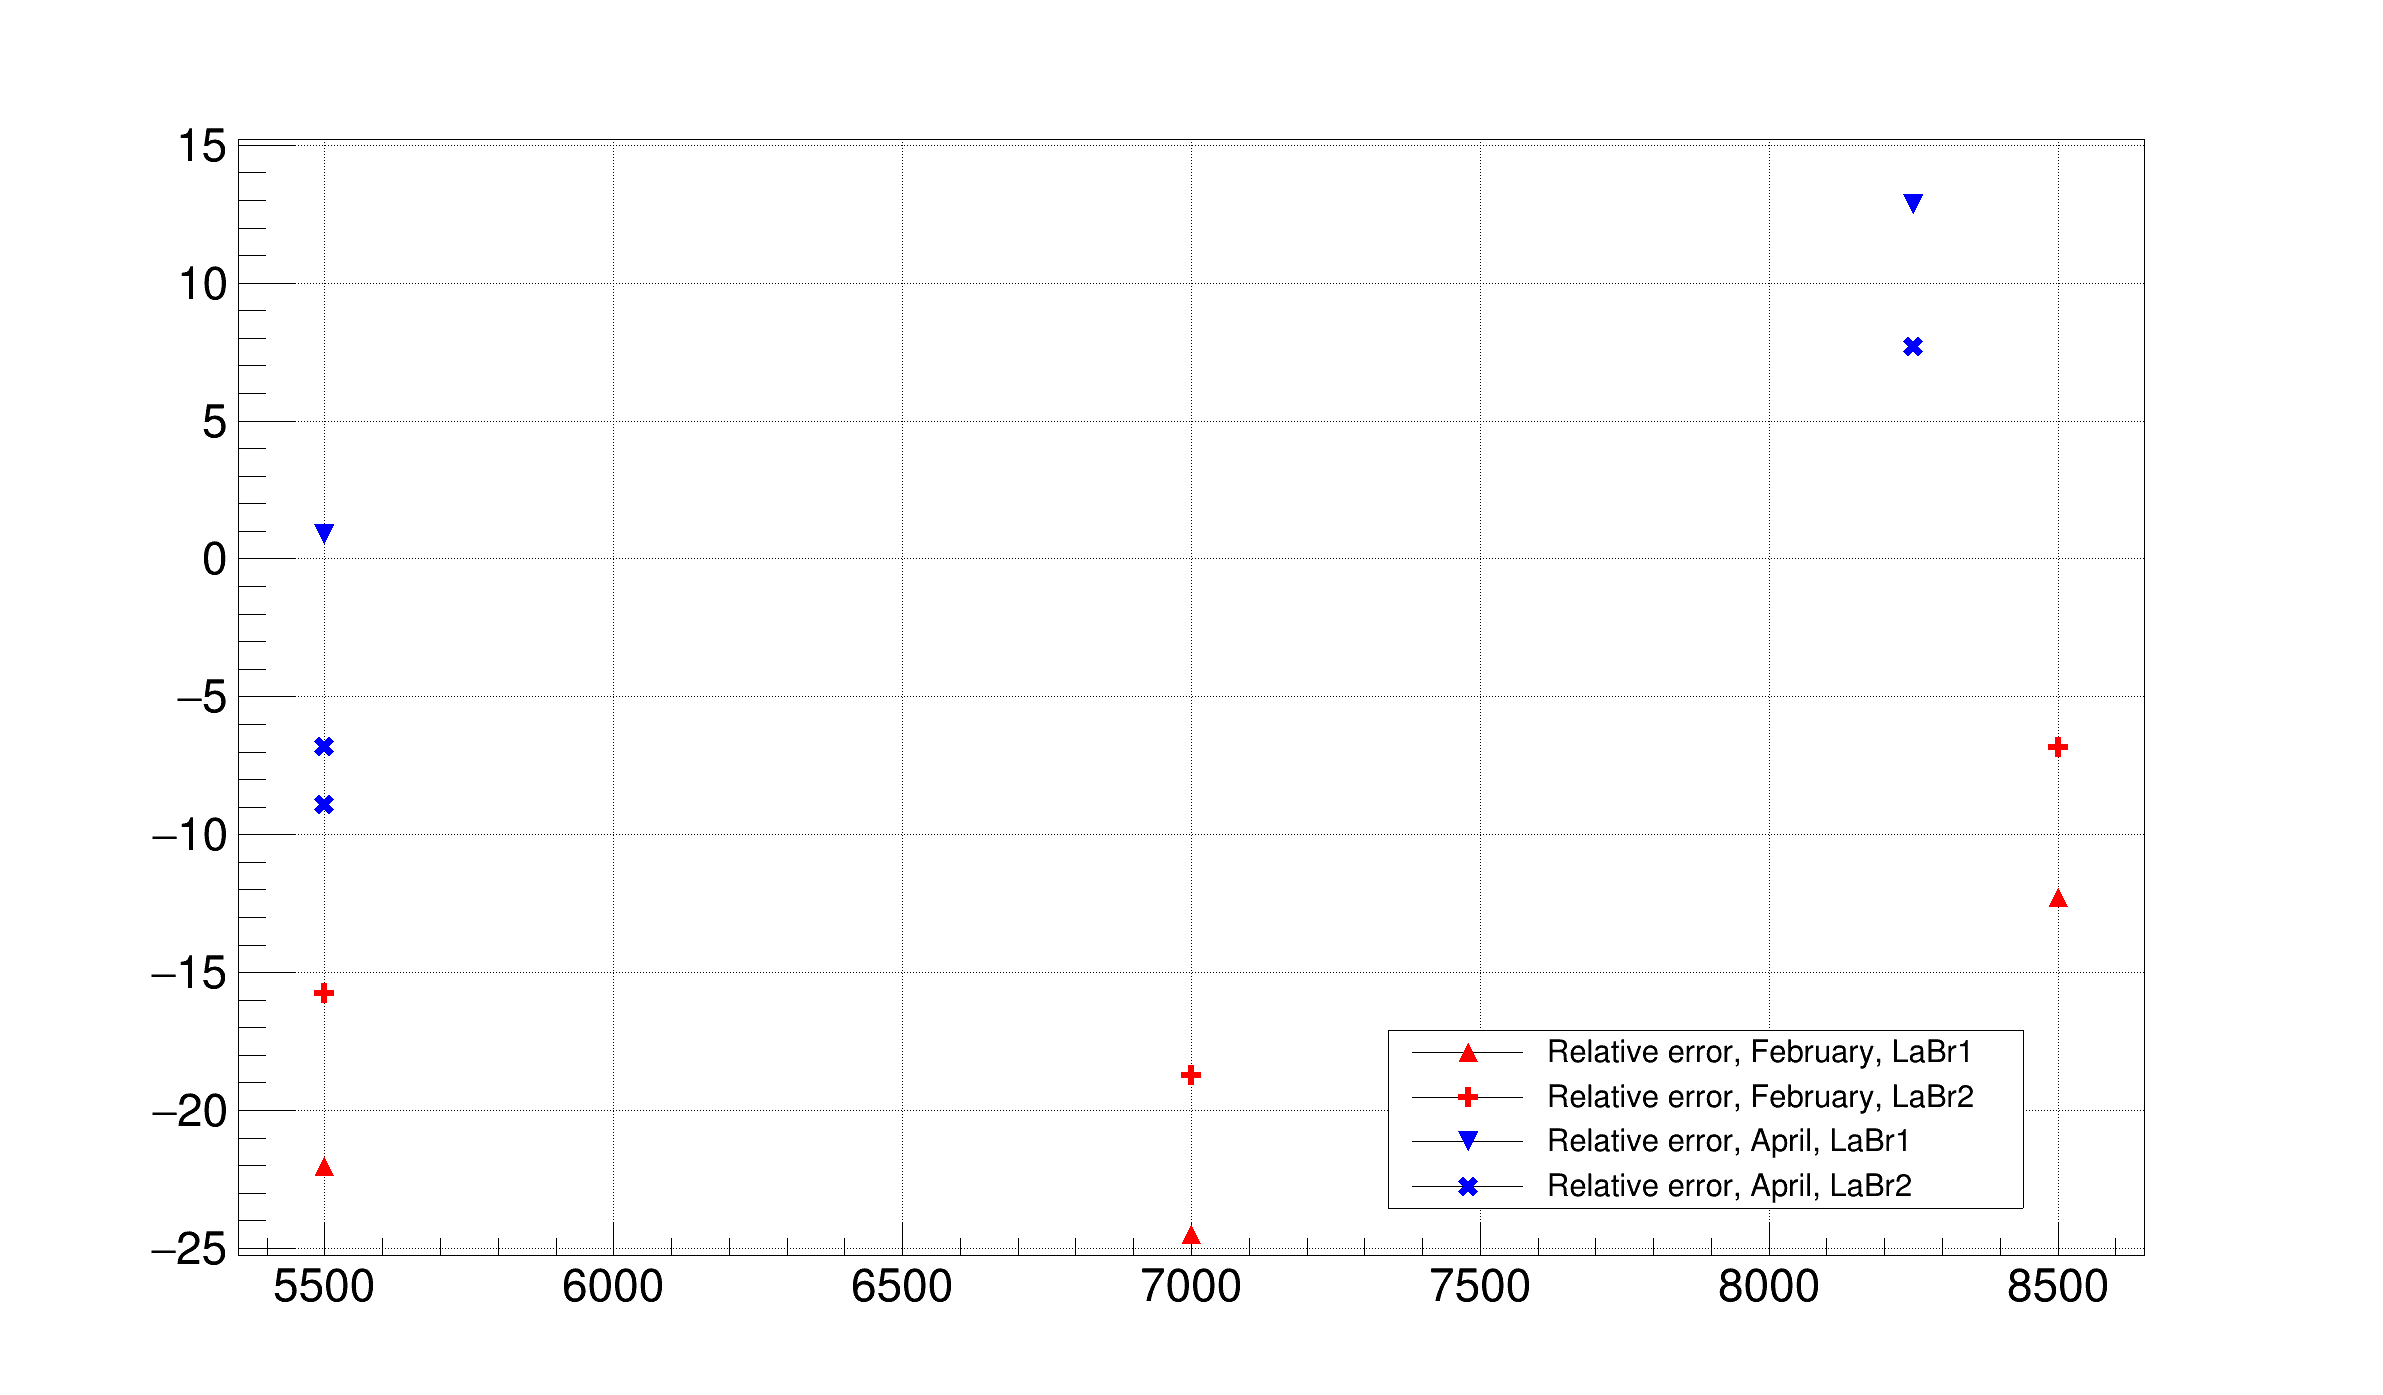
\includegraphics[width=\textwidth]{unified_errors_per.png}
	\caption{Percentage difference in thick target yield results between each \textit{unified} fit measurement and EXFOR.
	\textit{Outlier} measurement (LaBr1, measurement 6) at \qty{-60}{\percent} is not shown.}
	\label{unified_errors_per}
\end{figure}

For the \textit{unified} fits, errors are larger for February, but there is less difference than in the case of the \textit{decay} fits.
They are around \qty{10}{\percent} for April and \qty{20}{\percent} for February.

\begin{figure}[H]
	\centering
	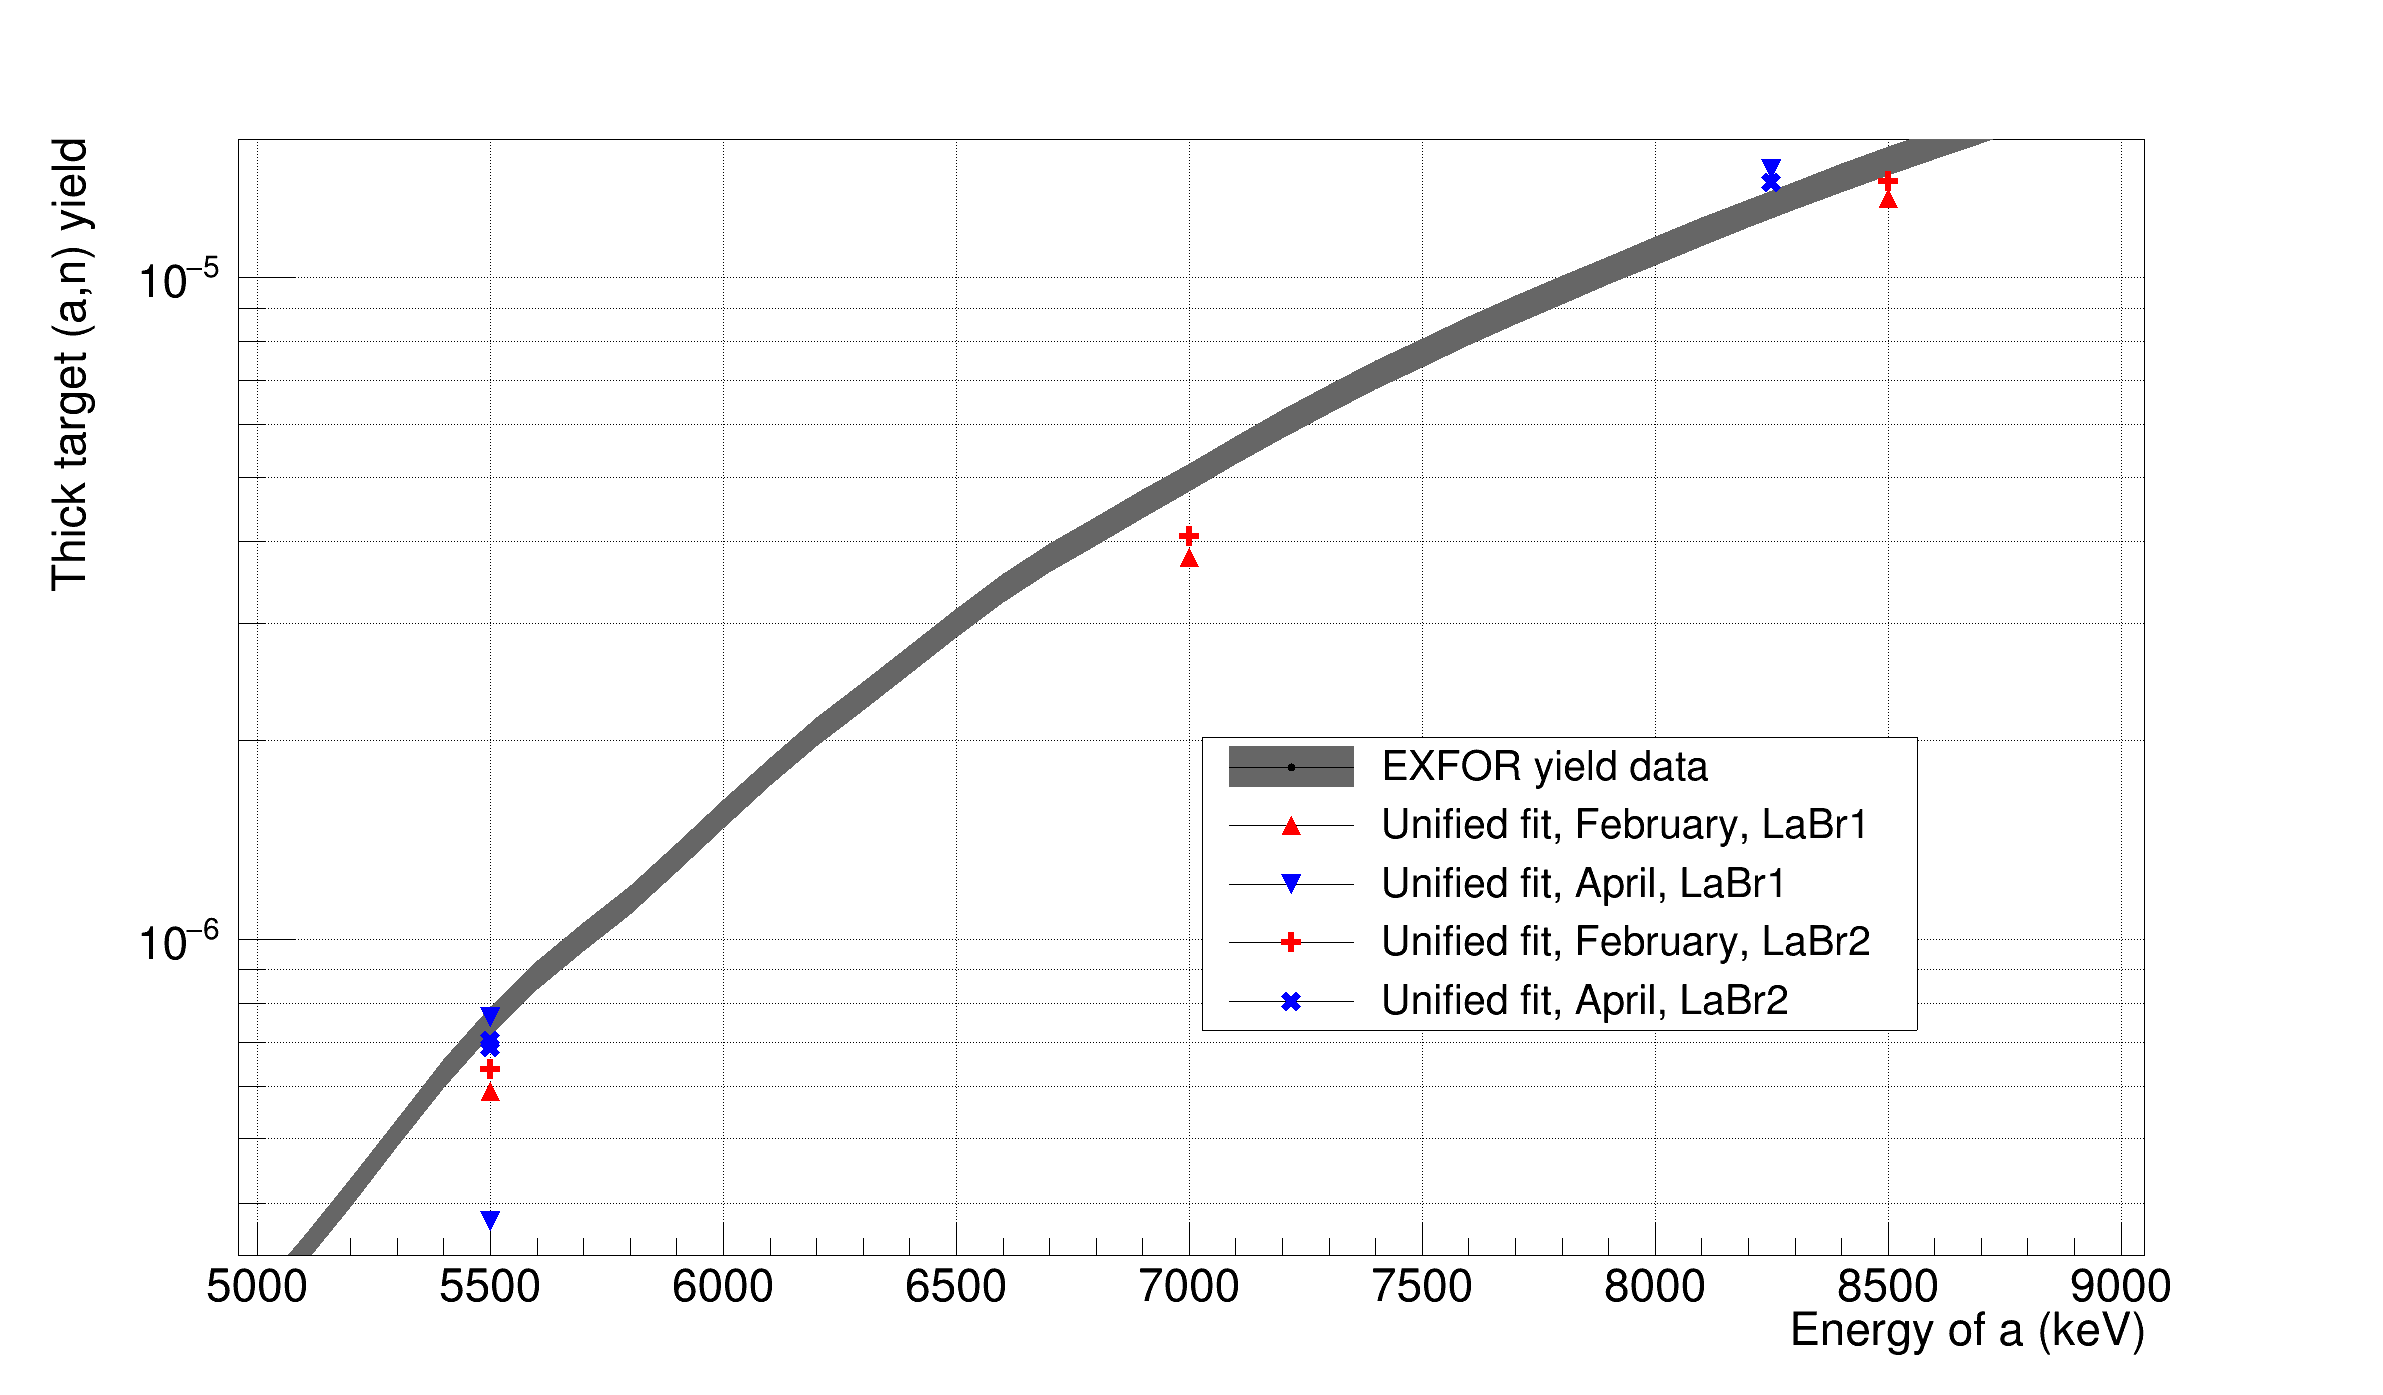
\includegraphics[width=\textwidth]{reactions_v_energy_unified.png}
	\caption{Unified fit results and EXFOR data with a \qty{\pm 10}{\percent} error.}
	\label{reactions_v_energy_unified}
\end{figure}

Putting all of the resulting thick target yields together with EXFOR data, we get figure \ref{reactions_v_energy}.
We see that April 18th \textit{decay} measurements agree well with EXFOR data, with \textit{unified} and \textit{rise} measurements have a larger error margin, and differ more.
\textit{Decay} February results, however, differ much more from all of the others.

\begin{figure}[H]
	\centering
	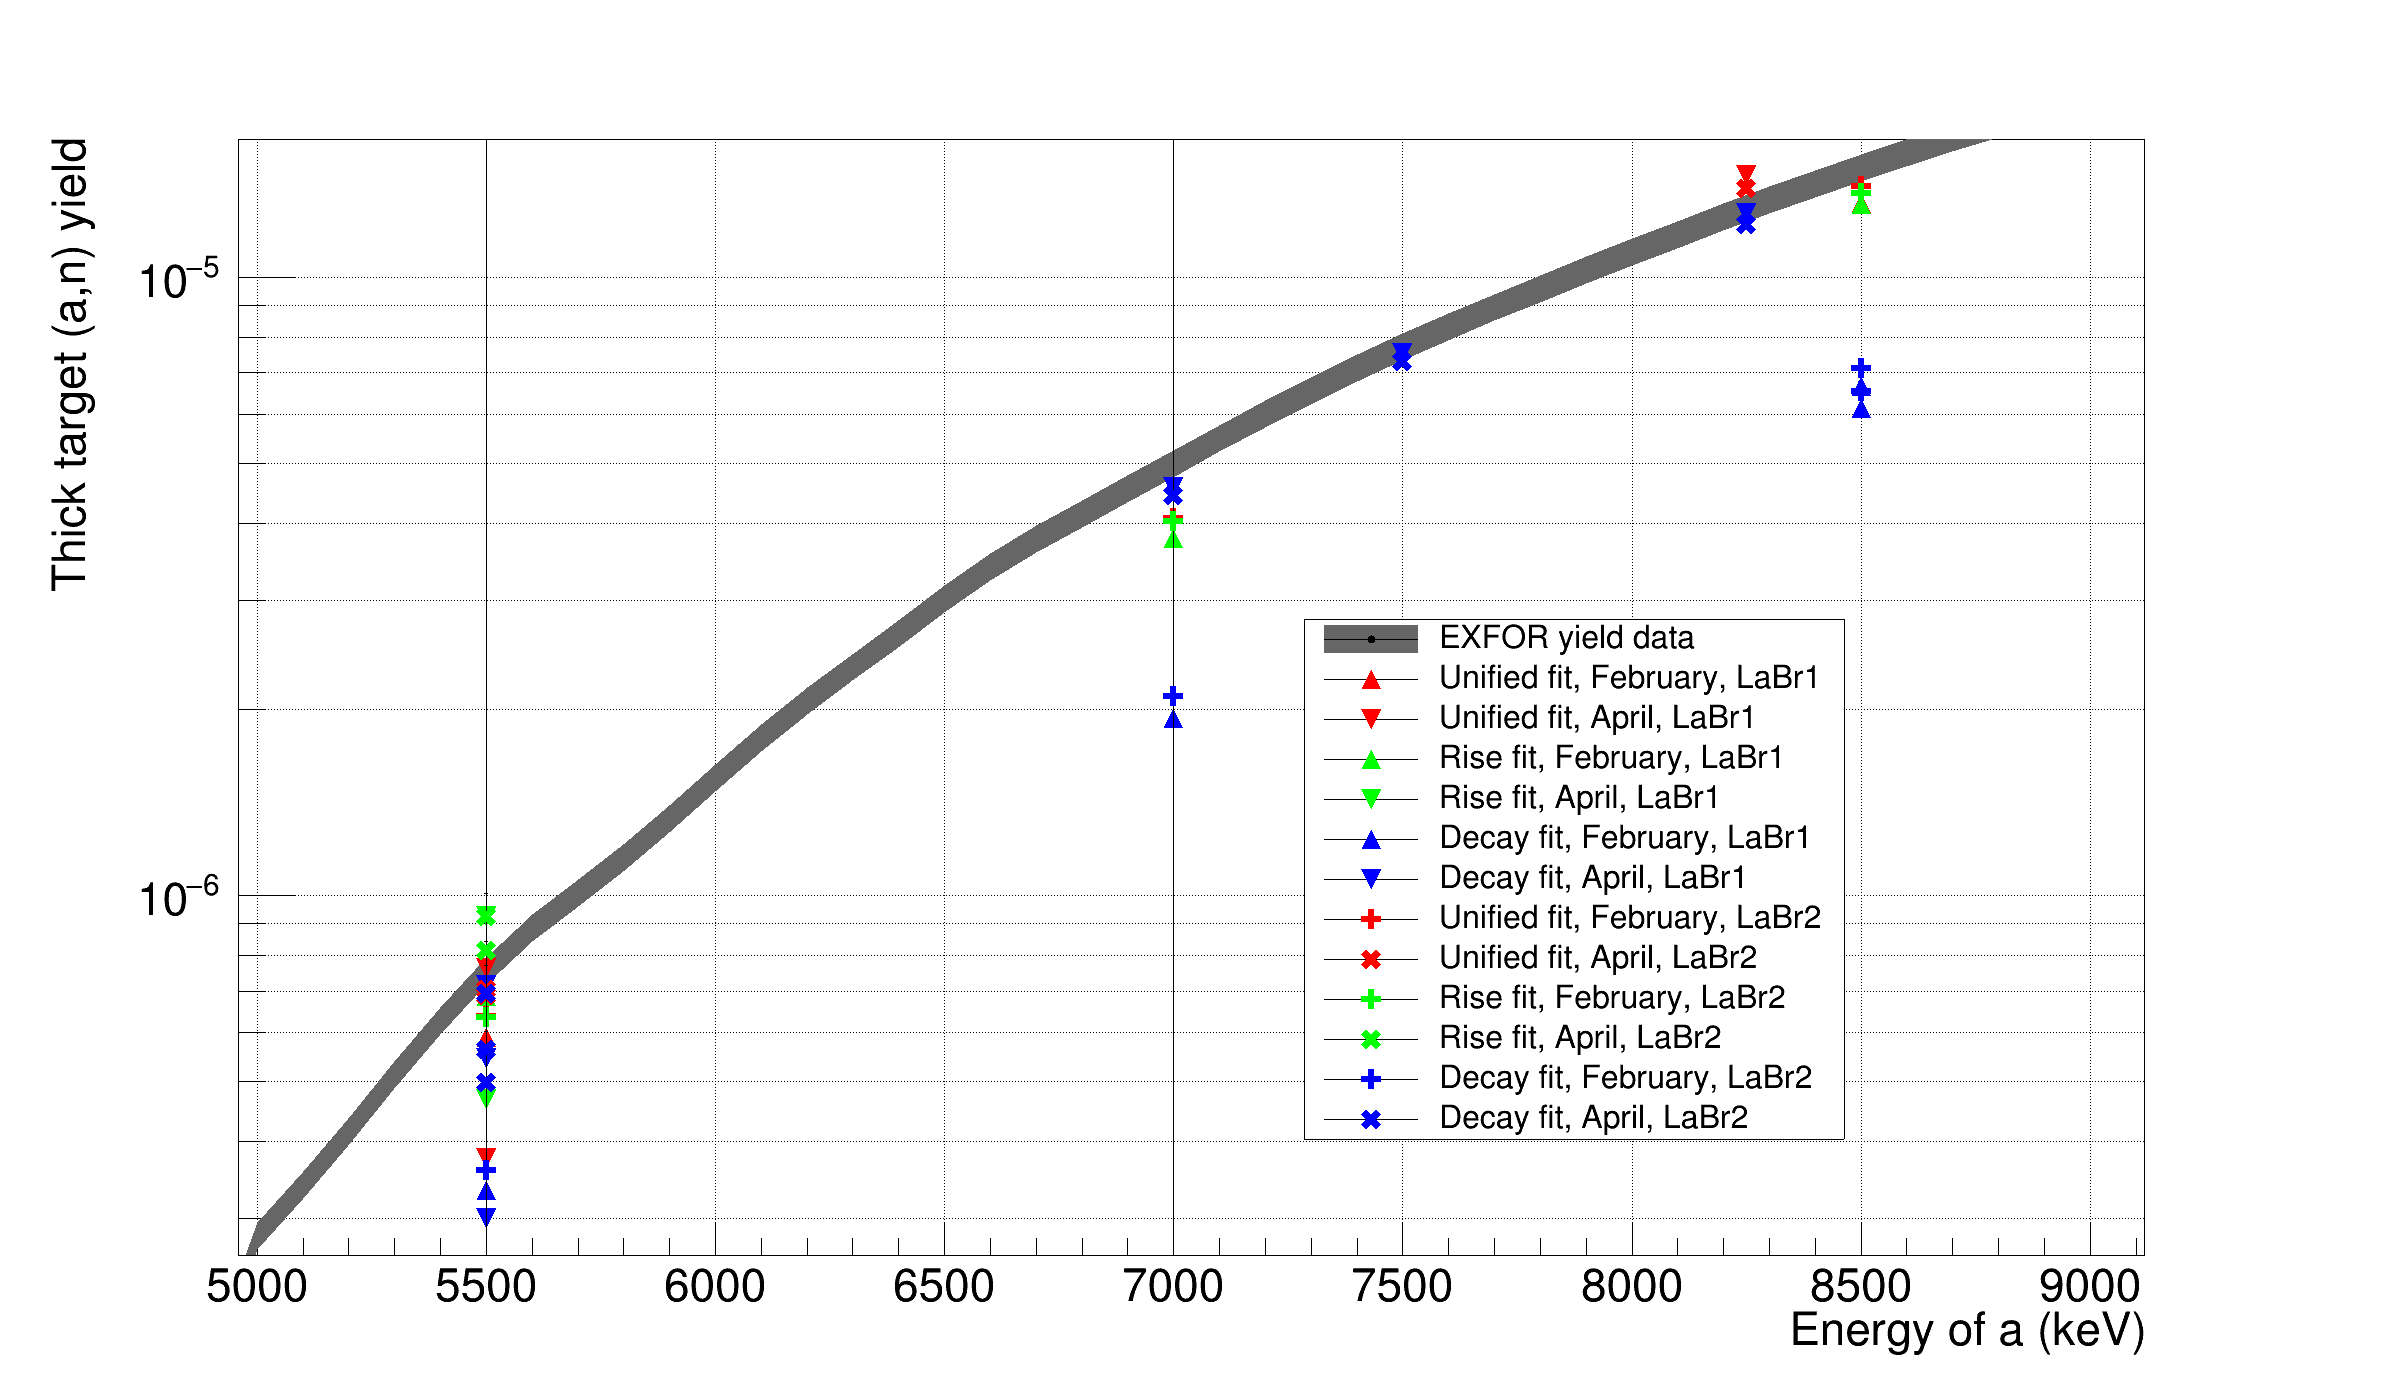
\includegraphics[width=\textwidth]{reactions_v_energy.png}
	\caption{All activation thick target yield results and EXFOR data with a \qty{\pm 10}{\percent} error.}
	\label{reactions_v_energy}
\end{figure}

This discrepancy of the \textit{decay} February measurements is unexplained.
If we ignore the February and April 17th \textit{decay} results, the measurements are around \qty{\pm 20}{\percent} of EXFOR.

\section{Pulsed}

\begin{table}[H]	%Tabla con datos de las medidas de haz pulsado
\centering
\begin{tabular}[c]{>{\bfseries}r||c|c|c}
	N& Energy (\unit{\keV}) & Distance (\unit{\meter}) & Date\tablefootnote{All took place in 2023} \\ \hline	%TBD?incertidumbre en distancia?
	1&\num{5500}&\num{1.0}&April 17th\\ \hline
	2&\num{5500}&\num{1.0}&April 18th\\ \hline
	3&\num{7000}&\num{1.0}&April 18th\\ \hline
	4&\num{8250}&\num{1.0}&April 18th\\ \hline
	5&\num{8250}&\num{2.0}&April 18th\\ \hline
\end{tabular}
\caption{Pulsed measurements}
\label{pulsed_measurements_table}
\end{table}

·We separate gamma flash and neutron response. Show tof histograms.\\
·Explain deconvolution:\\
·We fit the neutron response histogram to a function that takes as input the gamma flash histogram and 50 parameters corresponding to the neutron spectra in time of flight. The function loops through the gamma histogram to add the contribution of each bin.\\
·The result is to remove the effect of the width and assymetry of the gamma flash. Show plot of neutron response+response to delta.\\

·We convert the resulting parameters from time of flight to energy. Show energy spectra plot.\\
·We correct considering the efficiency of the detector. Show final plot.\\


\chapter{Conclusions}
·We have managed to measure \an reaction yield in \Aliso with X uncertainty (given different detectors, days or months) and X agreement with previous measurements.\\
·We have managed to measure the corresponding neutron energy spectra with X uncertainty/resolution and X agreement with previous measurements.\\

\begin{thebibliography}{5}
	\bibitem{nucleardatasheets}Nuclear Data Sheets 111, 2331 (2010), M. Shamsuzzoha Basunia.
\end{thebibliography}

\end{document}
